利用蒙特卡洛方法来计算光照传输积分方程,例如上一章讨论的路径追踪技术,是当前工业中主流渲染器正在使用的解决方案。路径追踪是一种简单,优雅,且易于实现的算法,它几乎能够实现全部全局光照效果。

然而路径追踪技术主要的问题是噪点非常严重,它来源于其估计的方差,并且由于蒙特卡洛估计方差和样本数量的关系(增加4倍的样本数量仅能够减少2倍的方差),它需要非常多数量的采样样本才能消除这些噪点,因此路径追踪算法的计算成本非常高;此外,同样由于样本数量的限制,那些小概率路径,例如SDS路径,也即是间接焦散(indirect caustic)\myindex{间接焦散}{indirect caustic}路径\footnote{焦散面是指光线由光源经过一次或多次光泽反射/折射之后进入的第一个漫反射面,此时如果摄像机能够直接观察到该焦散面,则称为直接焦散(direct caustic)\myindex{直接焦散}{direct caustic},即是$LS^{+}DE$路径,这种路径是可以被双向路径追踪采样的;但是对于间接焦散,即$LS^{+}DS^{+}E$,传统的路径追踪技术几乎完全无法处理。},如图\ref{f:pm-photon-maps-pros}(b)所示,传统的路径追踪几乎是不可能采样到的,而那些需要非常大数量的路径(例如漫反射光的多次反弹,如图\ref{f:pm-photon-maps-pros}(a)所示)也会因为采样数量的限制而导致噪点非常严重。

\begin{figure}
	\sidecaption
	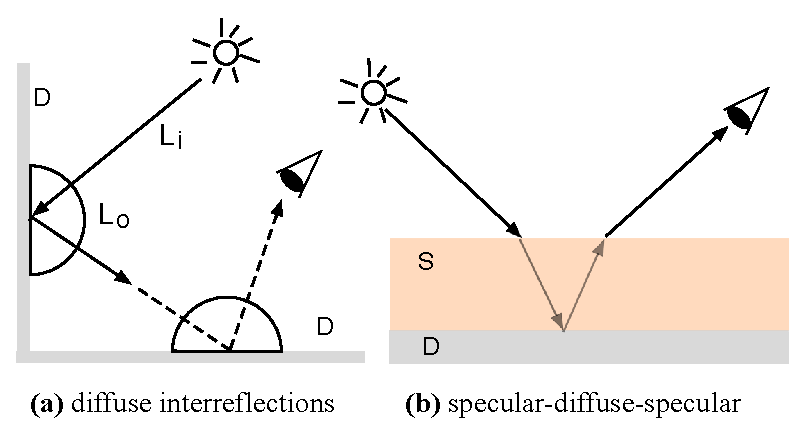
\includegraphics[width=0.65\textwidth]{figures/pm/photon-maps-pros}
	\caption{路径追踪在以下两个方面是低效的:(a)漫反射之间的交互需要远比光泽反射多得多的采样,因此噪点非常严重;(b)透过光泽面或半透明物体看到的间接焦散面的几率几乎为0。注意:传统的双向路径追踪是可以直接看到焦散面的}
	\label{f:pm-photon-maps-pros}
\end{figure}

光子映射是一种为改善蒙特卡洛路径追踪效率的替代技术。为了提高效率,它主要从两个层面对路径追踪进行改进:首先考虑到对于大多数模型(如漫反射表面),其辐射亮度场的变化在很大的面积范围内是非常平滑的,因此这些区域的光照信息可以被存储起来并重用;其次,也正是由于能够重用样本,我们可以使用类似于前面讨论的局部回归的思路\footnote{当然光子映射使用的密度估计是不同于回归的概念,但是它们在操作层面有一些相似,例如都能够对已有样本进行模糊来降低方差,本章后面将会区分和对比。},即光子密度估计,根据周围一定领域内的样本来近似计算某个位置的值,这使得我们可以得到一个更平滑(低噪)的结果。

然而和回归一样,这个模糊过程导致了估计的偏差,因此光子映射是一种有偏估计,但是这也大大提升了光子映射的效率,同时光子映射仍然满足一致性,这使得它也可以在增大样本数量的情况下得到正确的结果。高效性加上其处理焦散,多次漫反射反弹,参与介质等效果的能力,使得光子映射成为当前乃至未来一种重要的全局光照解决方案。





\section{数学基础}
在上一章,我们初步讨论了回归的概念,以及常用的一些回归方法,例如装箱法,局部平均回归,核估计以及多项式回归等等。所谓回归(regression)\mathindex{回归}{regression},就是用一定集合的已有抽样值,来拟合该集合隐含的一个真实的函数,例如核估计(kernel estimate)\mathindex{核估计}{kernel estimate}通过对周围一定领域范围内的样本求加权平均来计算某个位置的真实值。回归的结果必定伴随着模糊(或者平滑),而模糊导致(或增加)了偏差。然而,如果可以确定某个区域内某个函数值的变化是比较平坦的,则我们可以使用更少的样本值来进行拟合,这可以提高整体估计的效率。

这和本章光子映射技术使用的数学概念在某些方面有些类似,即密度估计。在统计学中,密度估计(density estimate)\mathindex{密度估计}{density estimate}就是基于一些观察数据构造出这些观察数据服从的概率密度函数(probability density function)\mathindex{概率密度函数}{probability density function}。最基本和最简单的密度估计方法称为直方图法(histogram method)\mathindex{直方图法}{histogram method},为了构造一个直方图,第一步就是将一定范围内的数据装入不同的箱(bin)中,即将数据按范围划分为多个连续的间隔,然后对每个间隔内的样本进行统计,如图\ref{f:pm-density-estimate}左边小图所示。这里的箱(间隔)必须是连续且不相交的,但是它们的尺寸可以相等或者不相等。这在某种程度上和局部回归中的装箱法(binning)\myindex{装箱法}{binning}有点类似,但是装箱法求样本的平均值,而直方图法求箱样本的和。

当对观察数据进行分箱并求和之后,形成的直方图就反应了观察数据的密度分布,每个箱的面积正比于该部分的频率,这可以通过图\ref{f:pm-density-estimate}左边小图可以看出。通过密度估计求得的概率密度函数通常是需要归一化的,然而在本章的例子中,其通过光子图估计出来的就是我们想要的场景中辐射能量的分布,因此并不需要对其进行归一化。

\begin{figure}
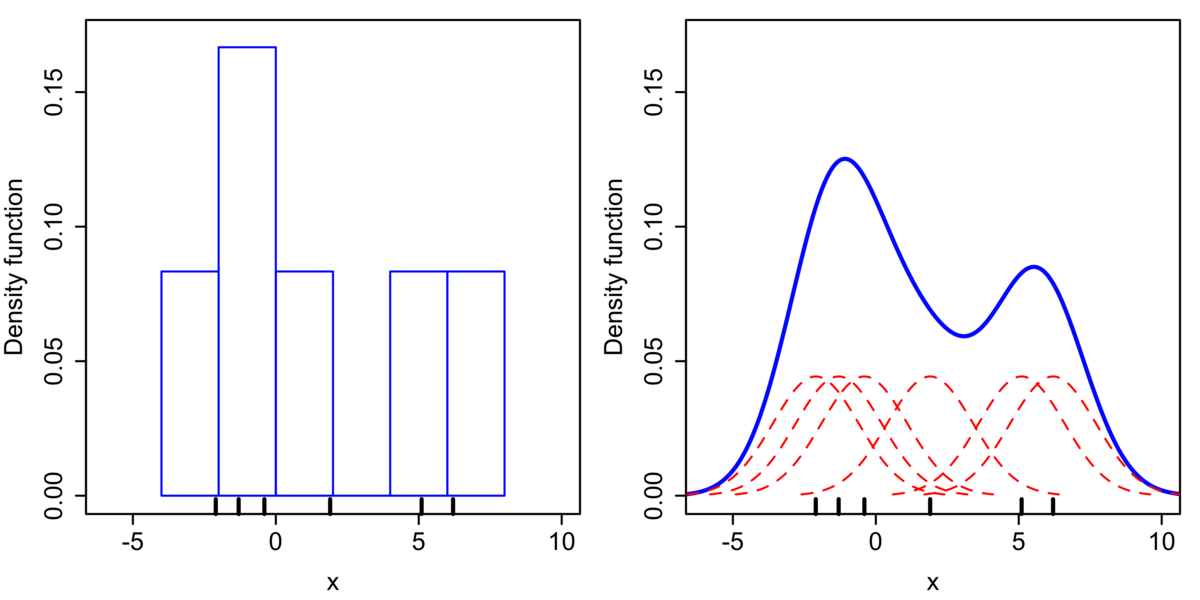
\includegraphics[width=1.0\textwidth]{figures/pm/density-estimate}
\caption{密度估计是对观察数据在不同区域上进行数量总和的统计,其结果能够反映该观察数据的密度分布。左图为最简单的直方图法,右图为核密度估计。其中横轴上的段黑线为数据点,红色虚线为核函数,蓝色曲线为核密度估计结果}
\label{f:pm-density-estimate}
\end{figure}

为了得到一个更平滑的密度估计,核密度估计(kernel density estimate)\mathindex{核密度估计}{kernel density estimate}方法对每个箱使用一个核函数来使箱之间密度的过度更平滑,如图\ref{f:pm-density-estimate}右边小图所示,其红色虚线表示核函数,它按照距离箱中心点的位置对每个样本分配一个不同的权重值。直方图法可以看做是最简单的一种核密度估计方法,其每个样本的权重都相等。

从以上的内容可知,密度估计和上一章讨论的局部回归(特别地,这里仅指和过滤概念一致的一阶局部单变量回归)本质上是不同的数学概念。但为什么我们要放在这里对比呢,这是因为两种技术都涉及对一个数据集中某个位置领域内的样本进行了模糊操作,例如求加权和,这是理解光子映射有偏性的重要基础。除此之外,本章后面光子映射技术和局部回归(或者过滤)不再有任何关系。

有了上述的数学基础,在还没有具体讨论光子映射技术之前,我们来思考一下它可以怎样被运用于光照传输中呢?密度估计所涉及的观察数据一定是具有任意可加性的,显然辐射亮度这种与方向有关的量是不便于累加的(否则每个样本都需要保持相同的方向),实际上光子映射中使用的被估计的数据是辐射通量,它是指单位时间内发出的能量,与具体面积和方向都是无关的,因此可以任意累加。

再往前一点,在光照计算中什么地方可以缓存辐射通量信息呢?在镜面或光泽表面肯定是不行的,因为缓存的从某个入射方向接受的辐射通量,按照另一个指定出射方向反射能量的几率几乎为0。所以,在光子映射中,我们仅在漫反射表面缓存辐射通量,这样它可以被任意累加(密度估计),然后这些能量可以(漫)反射到任意方向去,从而形成光照贡献。





\section{基本光子映射技术}\label{sec:pm-regular-pm}
光子映射可以追溯到\cite{a:Backwardraytracing}的反向光线追踪(backward ray tracing)\myindex{反向光线追踪}{backward ray tracing},由于当时还没有提出双向路径追踪这样的技术,因此Arvo的反向光线追踪主要用于实现从光源出发经过光泽面反射或折射光后到达漫反射表面的光照,这其实就是焦散效果(caustics)\myindex{焦散效果}{caustics},因为从摄像机出发的光线在最后经过光泽面之后几乎不可能反射或折射到光源上。

尽管都使用两个通道来实现最终的渲染,Arvo的反向光线追踪和双向路径追踪技术是有比较显著的区别的。反向光线追踪从光源发出的光束携带的不是辐射亮度(radiance),而是辐射通量(radiant flux),每个光束携带的能量是光源总能量的一部分,称为光子(photon),这些光子与场景的表面发生交互进行反射或折射,当光子到达漫反射表面时被记录,该光子的能量被累加到该物体对应的一个特殊的纹理中,称为光照图(illumination map)\myindex{光照图}{illumination map},光照图和普通物体表面的纹理是类似的,只不过它存储的是光照能量,而不是其他如法线,反射系数等量。

当前向的摄像机路径计算顶点的辐射亮度时,其漫反射分量可以直接从上述的光照图中获取,光照图中的纹素对应的入射辐射亮度可以根据辐射通量总和和其纹素的面积之间的联系推导而出(后面会具体讨论),该辐射照度的计算过程其实就是上一节讨论的直方图法。

自从被提出之后,光子密度估计就引起了研究社区极大的兴趣,\cite{a:GlobalIlluminationusingPhotonMaps}进一步使用k-NN最近邻估计代替之前的直方图法对光子密度进行估计,并且用一个独立的与场景无关的光子图(photon map)\myindex{光子图}{photon map}取代了与场景几何物体相关的光照图(一种特殊的纹理),此后此类方法统称为光子映射(photon mapping)\myindex{光子映射}{photon mapping}。




\subsection{光子追踪}\label{sec:pm-photon-tracing}
光子映射是一种双通道方法(two-pass method)。第一个通道通过从光源向场景中发射携带能量(辐射通量)光子开始,光子在场景中与物体表面进行交互(反射或折射),并在与非光泽面物体相交时被记录,最后所有这些光子被存储在一个光子图(photon map)\myindex{光子图}{photon map}当中,这个通道也称为光子追踪(photon tracing)\myindex{光子追踪}{photon tracing};第二个通道,也即是渲染通道,则使用传统的路径追踪技术从摄像机通过屏幕向场景中发射光线并在场景中传输,当光线与物体表面相交时,该顶点光照计算中的漫反射部分则使用统计的方法从前面产生的光子图中计算得出(即后面介绍的光子密度估计),这包括总的入射辐射通量的估计以及反射辐射亮度的计算。本节我们首先讨论光子追踪,在后面第\ref{sec:pm-radiance-estimate}节将会讨论光子密度估计。

光子追踪通道的目标是计算出非光泽表面的辐射通量分布,这主要包括三个步骤:从光源向场景中发射光子,追踪这些光子在场景中的传播,以及在非光泽表面存储这些光子。



\subsubsection{光子的发射}
首先,一个光子表述的是一个什么量?光子携带的是辐射通量(radiant flux),而不是传统光线追踪中使用的辐射亮度(radiance),它是每秒从光源发射出去的光源总能量的一个分数,例如给定一个$\Phi$瓦特的光源,一共发射出$N$个光子,则每个光子携带的能量为$ \cfrac{\Phi}{N}$瓦特,因此光子的能量与光源发射的光子数量有关,由于光源可以具有任意的形状以及辐射能量分布,这些发射的光子的密度分布应该服从光源辐射能量的分布,如图\ref{f:pm-photon-emission}所示。

\begin{figure}
	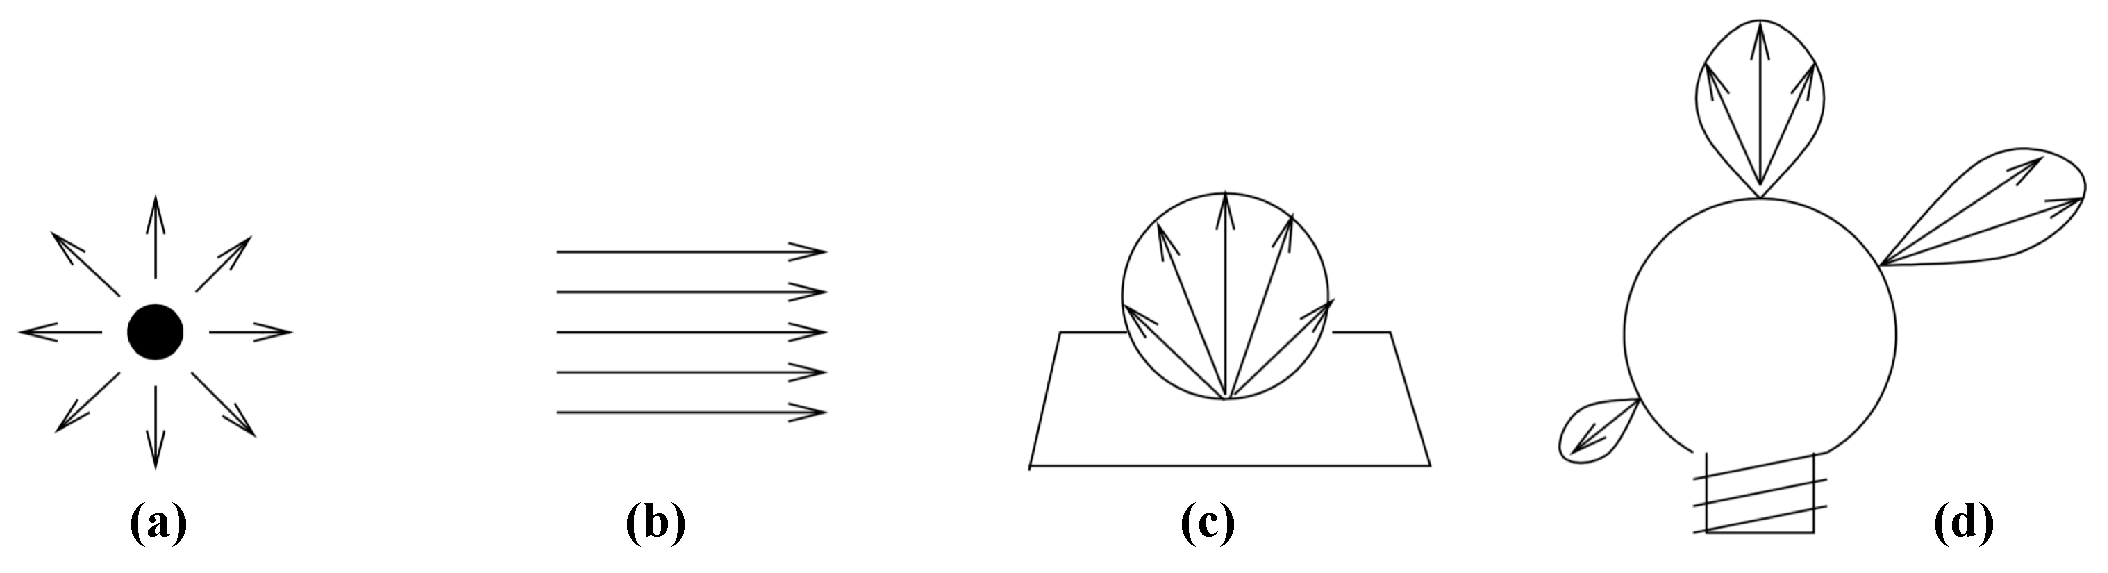
\includegraphics[width=1.0\textwidth]{figures/pm/pm-3}
	\caption{从不同类型的光源发射出的光子密度分布:(a)点光源, (b)直线光源, (c)矩形光源, (d)一般任意光源}
	\label{f:pm-photon-emission}
\end{figure}

例如对于点光源,光子从点光源所在的位置向整个空间方向均匀随机发射,如图\ref{f:pm-photon-emission}(a)及算法\ref{a:pm-diffuse-point-light}所示;对于直线光源,光子从超出场景外的位置沿直线光源的方向均匀地随机发射,如图\ref{f:pm-photon-emission}(b)所示;对于正方形光源,光子从正方形上一个均匀随机位置开始,以cosine分布向半空间方向发射,如图\ref{f:pm-photon-emission}(c)所示,越靠近垂直于平面的方向拥有更大的发射概率,而平行于平面的概率则为0。

\begin{algorithm}
\begin{lstlisting}[language=C++, mathescape]
emit_photons_from_diffuse_point_light() {
	$n_e = 0$ //发射的光子数量
 	while (not enough photons) {
		do { //使用取舍法对光子方向进行采样
 			x = random number between -1 and 1
			y = random number between -1 and 1
			z = random number between -1 and 1
		} while ( $x^{2} + y^{2} + z^{2} > 1$ )
 			
		$\vec{d}$ = < x , y , z >
		$\vec{p}$ = light source position
		trace photon from $\vec{p}$ in direction $\vec{d}$ 
 		$n_e =n_e +1$
	}
	scale power of stored photons with $1/n_e$ 
}
\end{lstlisting}
\caption{从一个均匀散射的点光源发射光子的算法伪代码}
\label{a:pm-diffuse-point-light}
\end{algorithm}

上述算法使用了取舍法来对光子方向进行采样,也可以使用任何能够满足光源辐射能量分布的函数进行采样。此外,每个光子的数据包含两个量:其携带的辐射通量(能量)以及光子传播的方向,这两个量都是后面用于估计光子辐射亮度的数据。





\subsubsection{光子在场景中的散射}
当一个光子被发射之后,它将按与光线追踪类似的方式在场景中传播,唯一的区别是光线追踪在每个顶点收集来自各个方向的辐射亮度,而光子传播的是辐射通量。当一个光子与物体表面相交时,它要么被反射,折射或者吸收,例如它不能同时包含反射和折射,这是不同于路径追踪中辐射亮度与表面的交互方式的\footnote{例如入射光可能部分被反射,另一部分被折射,因此一束光分散成多束光。},光子与表面的这种交互方式是根据物体表面的材质参数按概率的方式(如俄罗斯轮盘)确定的。

\begin{figure}
\sidecaption
	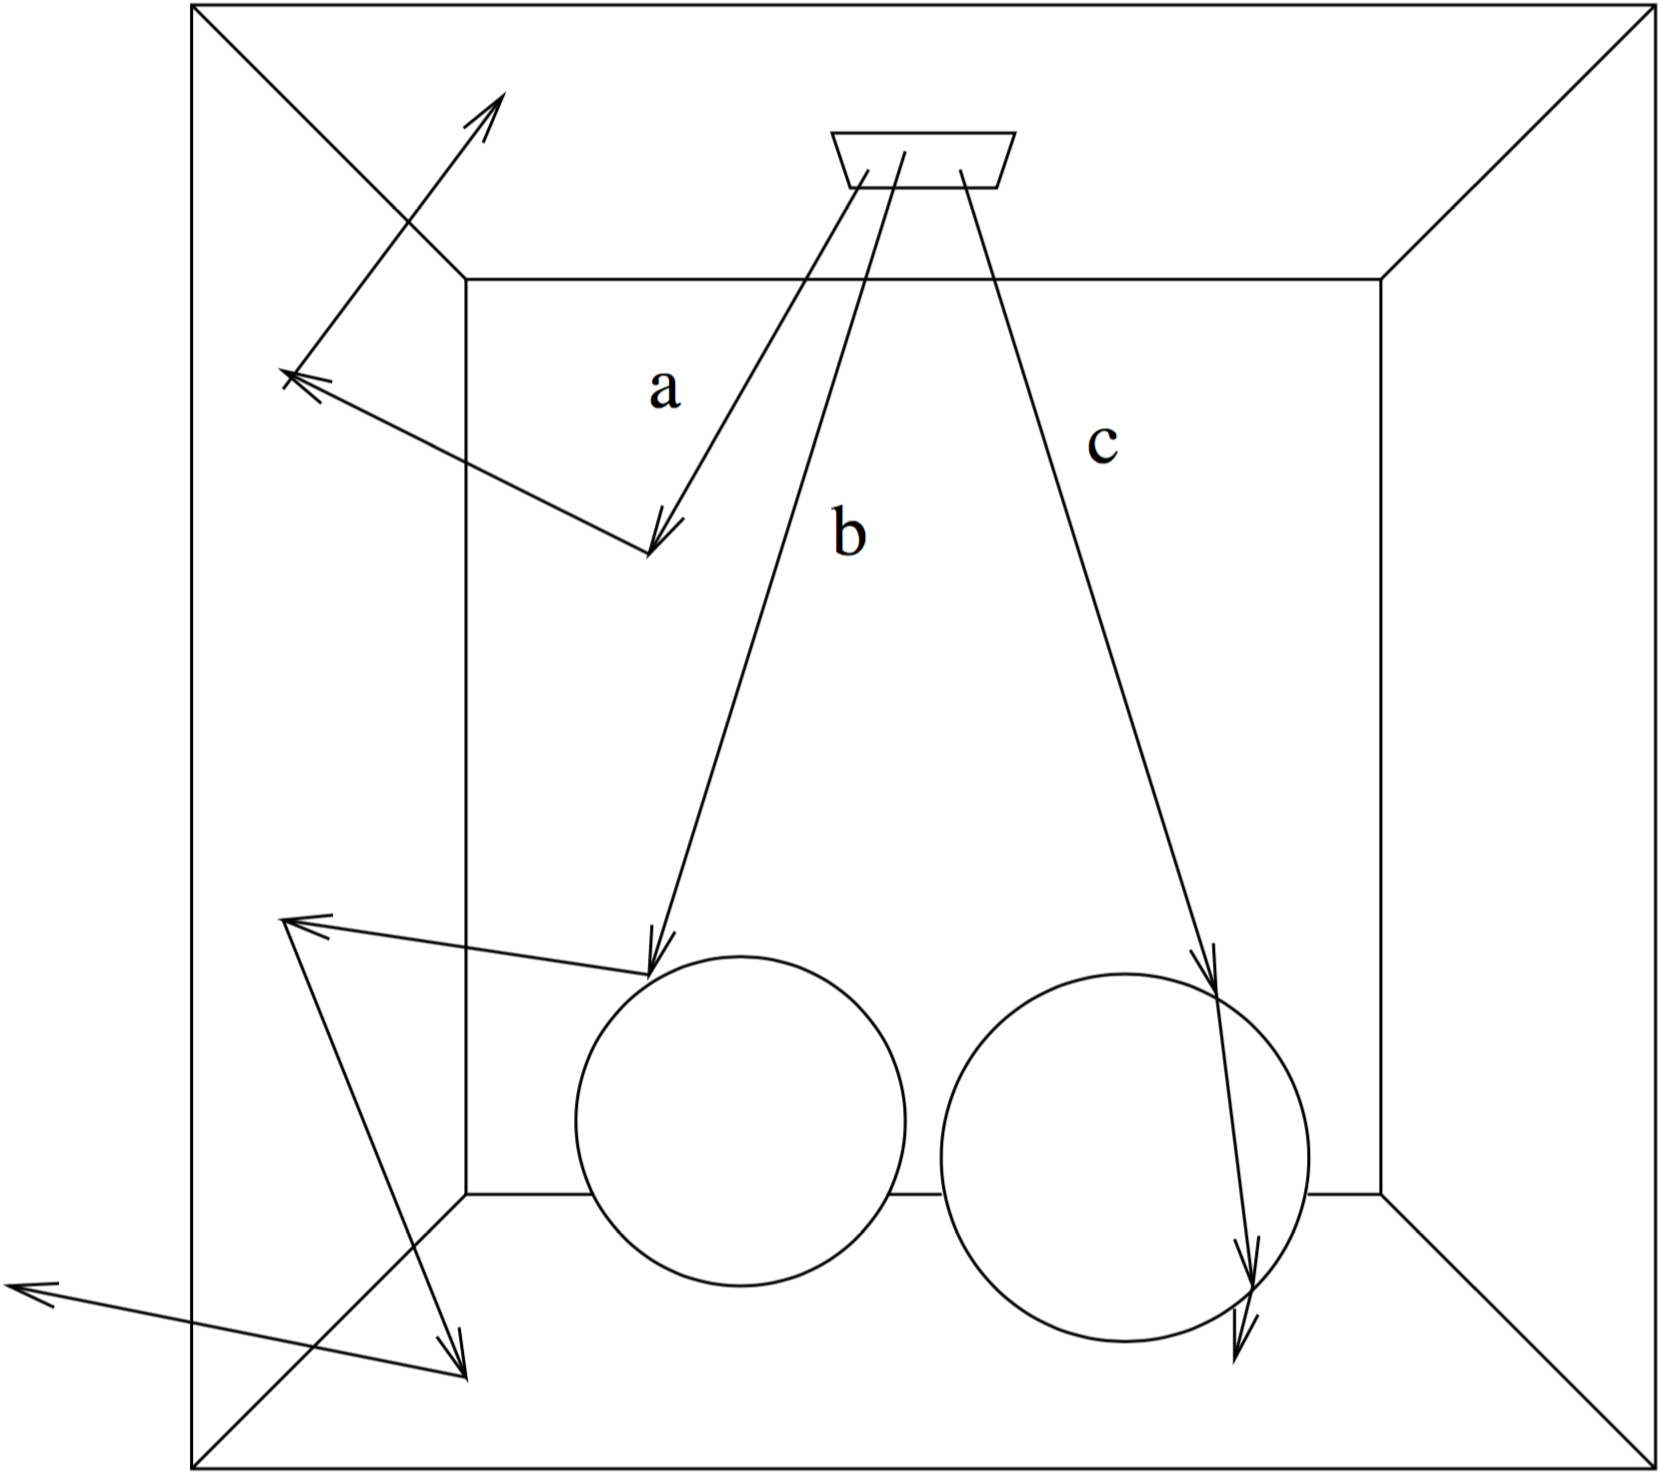
\includegraphics[width=.5\textwidth]{figures/pm/pm-4}
	\caption{光子在场景中的传播路径(Cornell盒子中包含两个球体,左边的球体为光泽面,右边球体为半透明的玻璃球): (a)两次漫反射之后被吸收,(b)一次光泽反射之后跟随着两次漫反射,(c)两次折射之后被吸收。光子在传播图中,每经过一次漫反射表面都会被光子图存储记录,直到被吸收}
\end{figure}

如果光子击中一个镜面,它将遵循反射定律反射光子到新的方向。给定法线$\vec{n}$,入射方向$\vec{\omega}^{'}$,以及反射方向$\vec{\omega}$,它们满足:

\begin{equation}
	\vec{\omega}=2(\vec{n}\cdot\vec{\omega}^{'})\vec{n}-\vec{\omega}^{'}
\end{equation}

\noindent 上述的规则同样适用于光泽反射。

如果光子击中一个漫反射表面,则该光子将被记录在光子图中与该漫反射表面的交点位置处(第\ref{sec:pm-photon-storing}节),然后从该交点的半空间方向随机选择一个(漫)反射方向继续传播(除非被吸收);对于其他任意BRDF模型表述的表面,新光子的方向应该根据该BRDF分布进行重要性采样进行选择,或者可以通过分析的方法得出。

那么光子在传播过程中的反射,折射或吸收是怎样被决定的呢?光子映射技术通常使用俄罗斯轮盘(Russian roulette)\myindex{俄罗斯轮盘}{Russian roulette}来解决这个问题。我们已经在上一章(第\ref{sec:russian-roulette}节)介绍过,俄罗斯轮盘被引入光线追踪技术中用于安全,无偏地移除由于多次反弹而使光照贡献率变得很低或不重要的光线,从而加速光线追踪的计算,否则为了保证无偏估计,我们需要追踪无穷的光线长度。俄罗斯轮盘同样被引入光子映射中用于以概率的方式决定光子与表面的交互:反射,折射或者吸收。

俄罗斯轮盘的基本思路是用概率的方法来移除一件事情的某些部分同时能够得到正确(无偏)的结果,它可以被看做是一种特殊的重要性采样技术,其中对于不重要(被移除)的部分其概率密度函数值为0。

例如对于一个包含反射率为$d$($d<1$)的表面,其入射光子的能量为$\Phi_p$,我们可以使用俄罗斯轮盘来决定光子是被反射或者被吸收,即:

\begin{equation}
	\Phi=\begin{cases}
		\xi<d  & \Phi_p\\
		\text{ 其他}  & 0
	\end{cases}
\end{equation}

\noindent 这里$\xi\in[0,1]$是一个均匀分布的随机变量。需要注意的是,上式和上一章中俄罗斯轮盘的使用方式不一样:存活下来(被反射)的光子并没有被除于存活概率(即使用重要性采样),这样做的目的是保证光子图中的光子能量尽可能相似,这可以减少后面辐射亮度估计的误差。这对于单个光子而言其结果虽然是不正确的,但是对于多个光子平均而言则是正确的,例如对一个具有反射率为0.5的表面发射1000个光子,我们可以反射1000个具有原始光子一半能量的光子,也可以反射500个和原始光子能量相同的光子,其平均而言结果都是相同的。

再例如对于一个同时包含光泽和漫反射的表面,其漫反射系数为$d$,光泽反射系数为$s$,其中$d+s\leq 1$,使用俄罗斯轮盘可以得到:

\begin{equation}
	\xi\in\begin{cases}
		[0,d]  & \longrightarrow\text{漫反射}\\
		]d,s+d]& \longrightarrow\text{光泽反射}\\
		]s+d,1]& \longrightarrow\text{吸收}
	\end{cases}
\end{equation}

同样的原理可以运用于折射或其他更复杂的场景,例如不同分量具有不同值的RGB颜色光源,以及对不同颜色通道具有不同反射率的材质等,可以从\cite{a:APracticalGuidetoGlobalIlluminationusingPhotonMaps}获得更多信息。

为什么使用俄罗斯轮盘的方式来决定光子的行为(反射,折射或吸收),而不是像路径追踪一样将光线按照反射分拆为多条光线,这样的处理方式是出于性能考虑。如同下一节将会看到的,所有光子会被存储到一个光子图中,因此对于如光泽表面,一个光子需要被反射或折射到多个方向,即一个光子分割成多个光子,例如每个光子每次与表面相交产生2个光子,则经过8次反弹之后一个光子将会产生$2^8=256$个光子,这大大增加了光子图存储的压力,显然这是比较糟糕的。

相比较于精确地使用反射或折射系数缩放和分拆光子的方式,但使用概率的方式来决定光子行为增加了方差,因为这里增加了一个采样的过程,但是随着光子数量的增加,这些方差会逐渐减少并使整个方案收敛到正确的结果。





\subsection{光子的存储}\label{sec:pm-photon-storing}
如前所述,当光子击中漫反射表面\footnote{这里不记录光泽或镜面表面光子的原因是,能够匹配这些入射光子与后面渲染通道中的给定方向的光线的概率几乎为0,所以对于包含大量光泽面或镜面的场景,传统的路径追踪技术更有效。}时,该光子会被记录在一个全局的数据结构中,称为光子图(photon map)\myindex{光子图}{photon map}。对于光子图,首先需要理解的是光子表述的是表面上的入射能量(通量),跟辐射亮度不一样,辐射通量是与面积(同时也和立体角)有关的量,这使得一个光子能够被用于近似表面上多个点的反射光计算;此外,被存储的光子的位置是位于物体表面上的,因此光子图间接反映了一个场景的所有漫反射表面的光照密度分布,如图\ref{f:pm-photon-storing}(b)所示,这也使得场景的(漫反射)光照表述可以与场景几何网格数据分离开来。

\begin{figure}
\begin{center}
	\begin{subfigure}[b]{0.492\textwidth}
		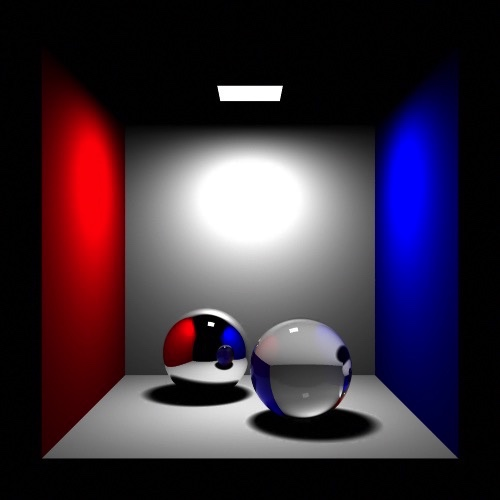
\includegraphics[width=1.0\textwidth]{figures/pm/pm-2-1}
		\caption{}
	\end{subfigure}
	\begin{subfigure}[b]{0.492\textwidth}
		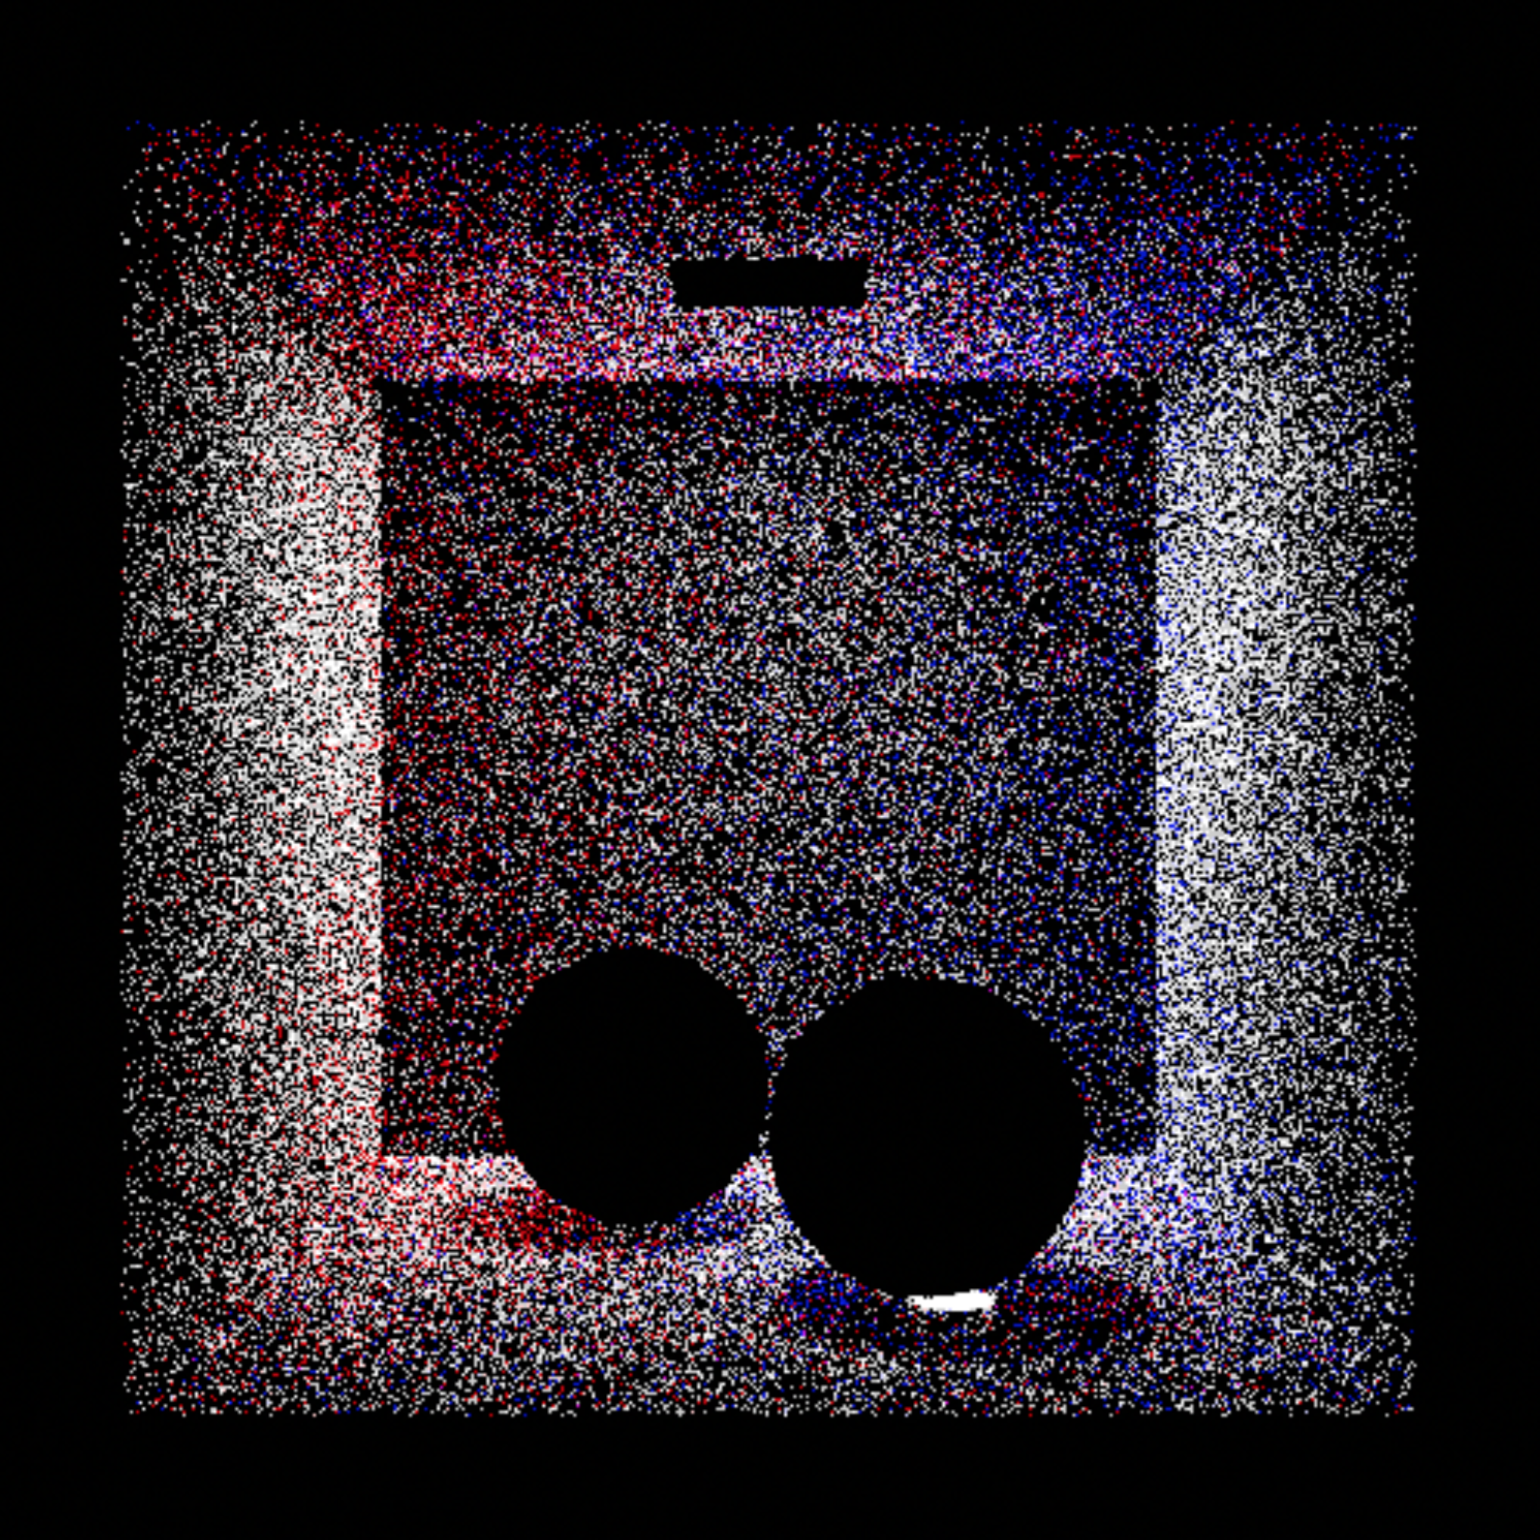
\includegraphics[width=1.0\textwidth]{figures/pm/pm-2-2}
		\caption{}
	\end{subfigure}
\end{center}
\caption{包含一个镜面球体(左)和玻璃球体(右)的Cornell盒子:(a)使用传统的光线追踪(包含直接光照,光泽反射和折射), (b)光子图中的光子密度分布。注意光线追踪技术忽略了玻璃球折射形成的焦散效果}
\label{f:pm-photon-storing}
\end{figure}

图\ref{f:pm-photon-storing}显示了一个一般场景,如图\ref{f:pm-photon-storing}(a)所示,与其对应的光子图,如图\ref{f:pm-photon-storing}(b)所示,从图中可以看出光子怎样近似了一个场景的漫反射表面入射能量,并且注意在光照更强的区域其光子密度更大,例如场景中右边球体下面(玻璃球折射形成的)焦散面处。

对于每个光子,其需要存储的数据包括光子位置(位于表面上),入射能量,以及入射方向,如算法\ref{a:pm-photon-data}所示。

\begin{algorithm}
\begin{lstlisting}[language=C++, mathescape]
struct photon {
	float x,y,z;     // 位置(3 x 32位浮点型 floats)
	char p[4];       // 编码的入射能量(4个字符)
	char phi, theta; // 压缩的入射方向 
	short flag;      // 用于光子图遍历的标志
}
\end{lstlisting}
\caption{光子图中一个光子的数据结构}
\label{a:pm-photon-data}
\end{algorithm}

在算法\ref{a:pm-photon-data}中,光子的能量是使用\cite{a:Realpixels}提出的4字符的RGB编码格式,当然如果内存足够的情况也也可以使用3个浮点型数据分别表示光谱的RGB三个颜色通道的能量(例如光源本身是带颜色的,或者场景包含对不同通道具有不同反射率的材质);flag标识用于表述后面会讲述的k-d树中每一级节点的分离面(例如x,y,或者z);入射方向是用球面坐标系表述,它们被映射为65 536个可能的方向,其计算方式如下:

\begin{equation}
\begin{aligned}
	phi&=255*({\rm atan2}(dy,dx)+PI)/(2*PI)\\
	theta&=255*{\rm acos}(dx)/PI
\end{aligned}
\end{equation}

通过后面的内容(第\ref{sec:pm-radiance-estimate-at-a-surface}节)可知,对于漫反射表面辐射亮度的计算是不需要知道入射方向的,已知辐射能量和该辐射能量对应的面积,就可以根据反射方向及BRDF反射系数求出出射辐射亮度。这里方向主要是用于\cite{a:RenderingcausticsonnonLambertiansurfaces}中对非漫反射表面的光照贡献计算。由于球面坐标系向笛卡尔坐标系的转换涉及计算量比较大的$\cos()$和$\sin()$计算,所以通常使用查表的方式来计算这些值。

当光子图生成之后,场景漫反射光照的表述便与场景几何数据分离开来,此后光子图作为一个独立静态的数据被用于后续光线追踪通道的辐射亮度估计。出于计算性能的需要,光子映射中常使用k-d树作为光子图的表述,我们在上一章已经介绍过k-d树,它是一只基于空间划分的树形结构,然而在那里并没有做什么的介绍,以下内容将讨论k-d树的表述,平衡化,查找算法及其复杂度。




\subsubsection{三种类型的光子图}\label{sec:pm-three-photon-maps}
出于性能考虑,实践中常把光子按照不同效果对光子密度的不同程度的要求拆分到三种不同类型的光子图中\footnote{当然这种划分主要是针对本节讨论的基本的光子映射算法,它在内存有限的情况下只能通过这种对采样密度要求的不同来划分光子图从而提高计算,然后对于后面讨论的如渐进式光子映射算法,它们本身能够克服基本光子映射内存限制的问题,因此它们往往使用单个更光子图类型即可。}:焦散光子图,全局光子图以及体积光子图。本节仅介绍前两者,体积光子图将在第\ref{sec:pm-participating-media}节介绍。

焦散光子图(caustic photon map)\myindex{焦散光子图}{caustic photon map}包含所有在击中漫反射表面之前至少经历过一次光泽或镜面反射的光子\footnote{实际上,现实生活中绝大部分人造光源(如白炽灯)都是被包含在某种形式的光泽物体(如玻璃球)内部,所以焦散是普遍存在的。},它们的路径可以表述为:$LS^{+}D$。 图\ref{f:pm-photon-maps}(a)显示了一个焦散光子图的构建,这些光子仅由光源向玻璃球方向发射,然后传播直到它们击中漫反射表面时停止并存储。

\begin{figure}
\sidecaption
	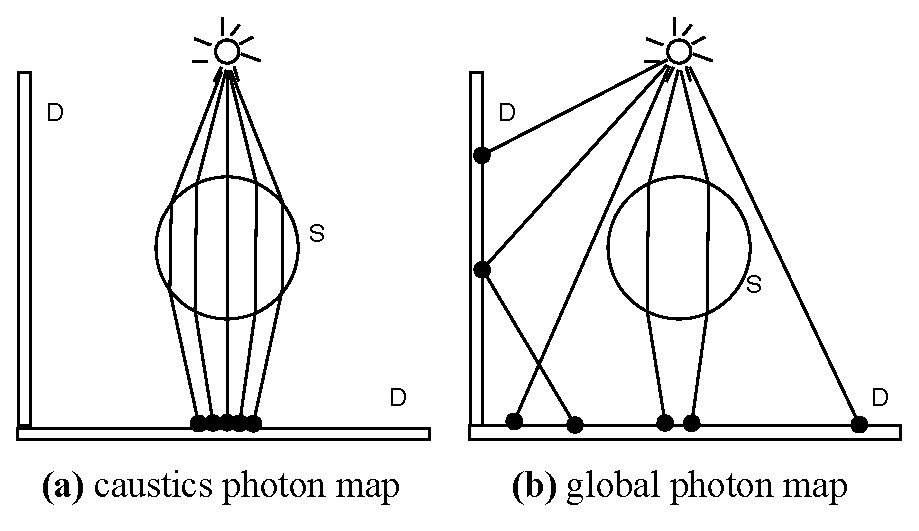
\includegraphics[width=.65\textwidth]{figures/pm/photon-maps}
\caption{构建不同类型的光子图,其中D表示漫反射表面,S表面镜面或光泽表面。注意:在(b)中一个光子可能存储于多个表面上}
\label{f:pm-photon-maps}
\end{figure}

由于焦散光子图中的光子是用于渲染能够直接被摄像机看见的焦散效果(见后面第\ref{sec:pm-rendering}节的介绍,当然它们也可以被用于渲染间接焦散面),以及焦散效果通常伴随比较明显的边缘形状,所以它需要使用很高的分辨率以避免噪点。尽管如此,由于焦散效果通常只发生在少数表面,并且焦散效果常常是一种聚焦的现象,所以焦散面的面积相对整个场景非常小,使用很少的光子数量就可以达到很好的效果,程序中通常可以通过标注哪些物体是光泽面以及哪些物体可以接受焦散光子(作为焦散面)来加速焦散光子图的构建。

全局光子图(global photon map)\myindex{全局光子图}{global photon map}包含所有击中漫反射表面的光照,如图\ref{f:pm-photon-maps}(b)所示,全局光子图同时包含直接光照,间接光照以及焦散效果,它们的路径可以表述为:$L\{S|D|V\}^{*}D$)。需要注意,焦散光子图和全局光子图中可能包含相同的光子,这通过对比如图\ref{f:pm-photon-maps}(a)和\ref{f:pm-photon-maps}(b)可以看出,所以一个面不可以同时使用这两个图渲染相同的效果,具体内容将在第\ref{sec:pm-rendering}节介绍。





\subsubsection{k-d树}
\cite{a:MultidimensionalBinarySearchTreesUsedforAssociativeSearching}首次将k-d树引入计算机图形学中,它是一种特殊的二叉树,由于每个节点存储的是一个$k-$维数据,故称为k-d树(k-d tree)\myindex{k-d树}{k-d tree}。

在构建k-d树的时候,与标准的二叉树相同的是,它通过对数据进行迭代细分来实现;然而,与标准的二叉树仅使用一个标准键(如x轴)对所有层级的节点进行细分不同的是,k-d树对每个层级使用一个不同的划分依据键,一个k-维的k-d树一共使用k个不同的键,并分别对不同的层级使用不同的键并如此循环。

\begin{figure}
\begin{center}
	\begin{subfigure}[b]{.49\textwidth}
		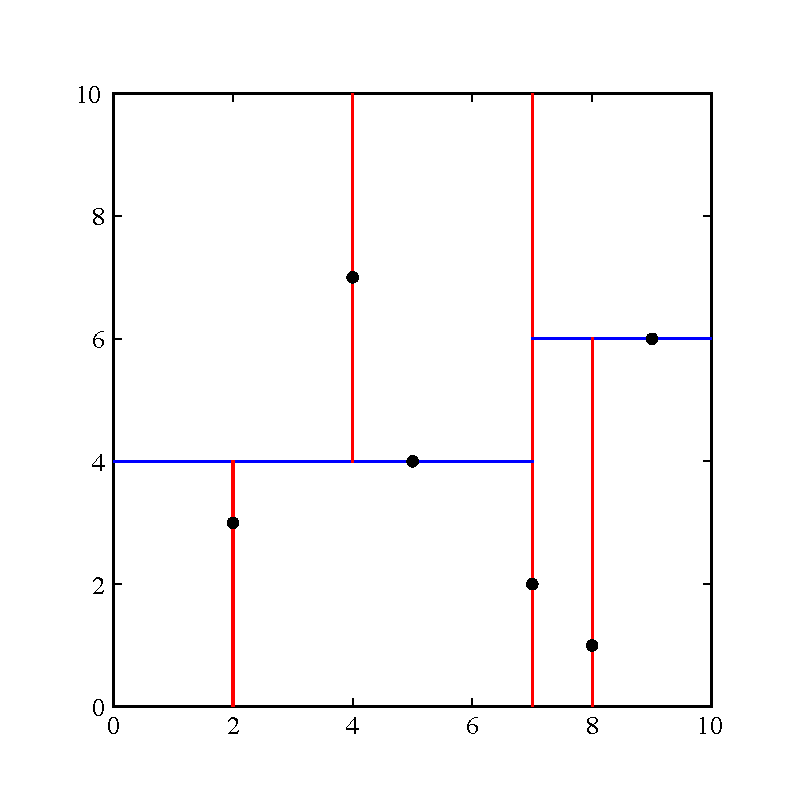
\includegraphics[width=1.0\textwidth]{figures/pm/k-d-tree-1}
		\caption{}
	\end{subfigure}
	\begin{subfigure}[b]{.49\textwidth}
		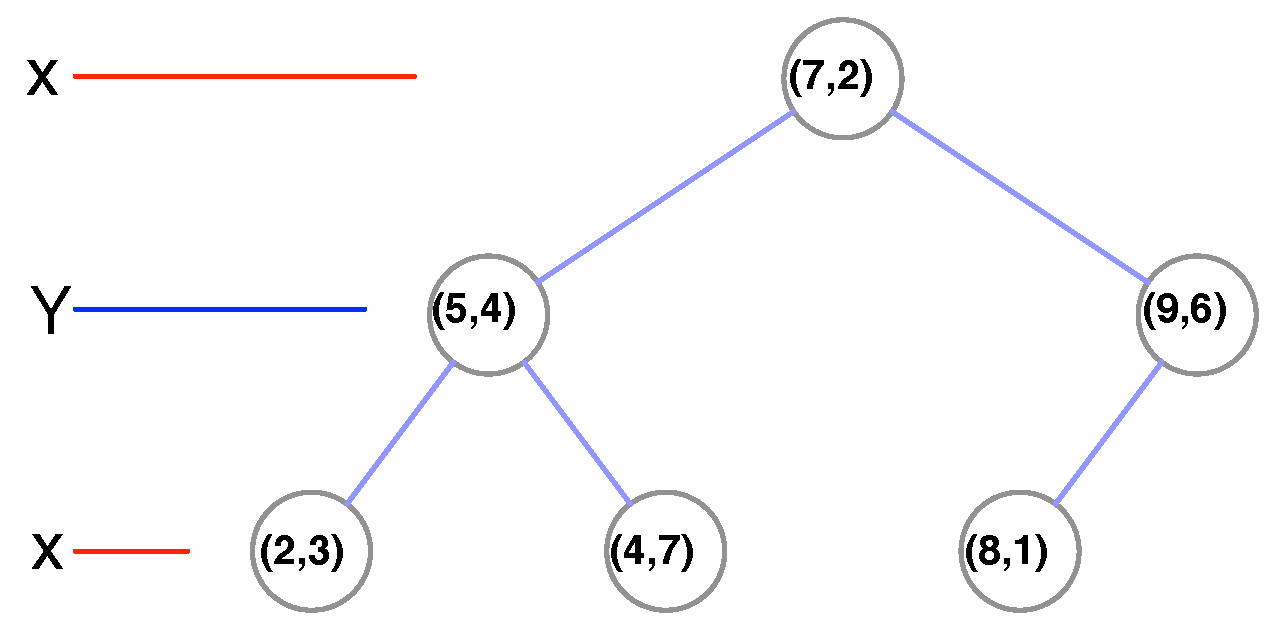
\includegraphics[width=1.0\textwidth]{figures/pm/k-d-tree-2}
		\caption{}
	\end{subfigure}
\end{center}
\caption{(a)k-d树的细分过程,其2维点数据集合为:$(2,3), (5,4), (9,6), (4,7), (8,1), (7,2)$,(b)为构建的k-d树}
\label{f:pm-photon-kd-tree}
\end{figure}


例如对于一个3维的k-d树,其每个数据是一个3维坐标(x, y, z),则构建的k-d树从上至下每个层级使用的键可能以下是循环列表:x, y, z, x, y, z...。图\ref{f:pm-photon-kd-tree}显示了一个包含2维数据的k-d树的结构,在图\ref{f:pm-photon-kd-tree}(b)中可以看出其每个层级分别使用不同的键对节点数据进行细分。

在k-d树中,每个节点都是数据集合中的一个数据,在本节即是一个光子。每个非叶节点隐式地充当了将所有子节点细分为两个子空间的超平面(hyperplane)\myindex{超平面}{hyperplane},其中每个子空间称为一个半空间(half-space),它包含一课子树,因此每个节点还包含分别指向这两个子树的指针。超平面的方向按照这样的规则选取:每个节点对应k-维中的某一维,使得超平面与该维对应的坐标轴垂直,这个选取的维称为一个键。例如,某个节点选取的键为"$x$",则它的左子树的所有节点的x坐标值小于该节点的$x$坐标值,而右子树种所有节点的$x$坐标值大于该节点的x坐标值。如图\ref{f:pm-photon-kd-tree}所示。

给定一个点集合,以下算法使用中值细分法构建一个k-d树:

\begin{algorithm}
\begin{lstlisting}[language=C++, mathescape]
kdtree *build_kdtree (list of points pointList, int depth) {
    // 基于深度循环地选取不同的坐标轴作为键
    int axis = depth / k;
        
    // 根据选取的键对输入点集合进行排序,并找到中点
    select median by axis from pointList;
        
    // 创建节点及子树
    node.axis = axis;
    node.location = median;
    node.leftChild = kdtree(points in pointList before median, depth+1);
    node.rightChild = kdtree(points in pointList after median, depth+1);
    return node;
}
\end{lstlisting}
\caption{构建一棵平衡k-d树的伪代码,由于k-d树每一级都使用不同的键来细分子节点,所以每一个节点都要重新对节点进行排序,构建复杂度较高}
\label{a:pm-balancing-photon-map}
\end{algorithm}

上述以集合中的中点为细分点的方式构建的k-d树称为平衡k-d树(balanced k-d tree)\myindex{平衡k-d树}{balanced k-d tree},\cite{a:MultidimensionalBinarySearchTreesUsedforAssociativeSearching}显示在一棵平衡k-d树中定位一个(最近位置的)节点的复杂度最坏的情况是$O(\log n )$,其最近邻搜索的效率最高,这里$N$是k-d树中所有节点的数量。

然而,由于在k-d树构建的过程中,每个层级的节点都需要使用不同的划分标准键,所以一个预先排好序的节点列表对于平衡k-d树的构建并没有多大帮助,如算法\ref{a:pm-balancing-photon-map}所示,为了构建平衡的k-d树,每个节点都需要按照当前节点的键进行重新排序,以获取集合中的中点。\cite{a:MultidimensionalBinarySearchTreesUsedforAssociativeSearching}显示在如果从一个包含$n$个点的集合中查找中点的复杂度是$O(n)$,则其构建的复杂度为$O(n\log n)$,然而实际上中点获取最糟糕的情况为$O(n^2)$,这使得构建平衡k-d树的复杂度更高。\cite{a:BuildingaBalancedkdTreeinOknlognTime}介绍了一种复杂度为$O(kn\log n)$的平衡k-d树构建算法。





\subsubsection{最近邻光子查找}
在后面介绍的光子密度估计计算中,需要使用k最近邻(k-nearest neighbors,kNN)\myindex{k最近邻}{k-nearest neighbors}估计计算辐射亮度,它需要获取一个给定位置附近的k个最近的光子,这就涉及k-d树的最近邻查找算法。

一般的最近邻查找算法通常从根节点开始遍历,如果当前节点与指定位置的距离在一定的距离范围内(一个保守的初始范围,超出该范围的节点被排除),则将当前节点添加到一个列表中,对于k个最近邻节点的查找,该列表的长度为k。在插入当前节点的时候,如果列表中已经包含k个元素并且距离最远的节点比当前节点的距离更大,则删除列表中最远的节点再插入当前节点,否则当前节点被丢弃。具有这种特性的列表可以称为最大值堆(max-heap)\myindex{最大值堆}{max-heap},它会持续跟踪堆中的最大值。当最大值堆中的元素填满时,我们可以使用该堆中最远的距离作为后续遍历的范围限定距离,以忽略一些k-d树距离比该最大距离更远的节点。算法\ref{a:pm-range-searching}\cite{a:APracticalGuidetoGlobalIlluminationusingPhotonMaps}展示了上述最近邻搜索算法的伪代码。

\begin{algorithm}
\begin{lstlisting}[language=C++, mathescape]
locate_photons( p ) {
	if ( 2p+1 < number of photons ) { 
		//遍历子节点
		//计算当前节点与x之间在当前节点细分键上的距离(即x到超平面之\ 间的距离)
		$\delta$ = signed distance to splitting plane of node n 
		if ($\delta$<0) {
			//搜索左子树
			locate photons( 2p ) 
			if($\delta^{2}<d^{2}$ )
				locate photons( 2p + 1 ) //检查右子树 
		} else {
			//搜索右子树
			locate photons( 2p + 1 ) 
			if($\delta^{2}<d^{2}$ )
				locate photons( 2p ) //检查左子树
		}
	}
			
	//处理当前节点
	$\delta^{2}$ = squared distance from photon p to x
	if ( $\delta^{2}<d^{2}$ ) { //检查当前节点是否足够近
		insert photon into max heap h
		// 调整最大限定距离为堆中元素的最大距离
		$d^{2}$ = squared distance to photon in root node of h 
	}
}
\end{lstlisting}
\caption{最近邻搜索算法。给定一个光子图,一个位置$x$,以及一个最大搜索距离$d^{2}$,该算法递归地遍历k-d树并返回一个包含指定数量个最近邻光子的堆$h$。其中locate\_photons(1)开始从根节点初始化搜索算法的计算}
\label{a:pm-range-searching}
\end{algorithm}

在上述算法中,直接使用了距离的平方$d^2$而不是$d$避免了平方计算。





\subsection{辐射亮度估计}\label{sec:pm-radiance-estimate}
光子映射技术中最最要的部分就是根据光子图对非光泽表面上任意点和任意方向进行辐射亮度估计(radiance estimate)\myindex{辐射亮度估计}{radiance estimate},对于给定位置和反射方向,它能够将光子图中带有辐射能量的光照转换为辐射亮度,这种估计的本质也使得它和光线追踪是两种比较独立的框架。

第\ref{sec:pm-radiance-estimate-at-a-surface}节将介绍一般的辐射亮度估计方法,而在之前了解为什么要进行光子密度估计也许更有益于理解辐射亮度估计的本质(第\ref{sec:pm-why-radiance-estimate}节)。




\subsubsection{为什么需要估计}\label{sec:pm-why-radiance-estimate}
如后面的内容可知,基本的辐射亮度估计其实是非常简单的,然而为什么要使用估计的方法(而不是如路径追踪中使用的顶点连接等),一般的相关资料则很少说明,这个问题虽然简单,但是额外的说明对于后面知识的理解还是有帮助的。

所谓估计,在统计学中一般是指用一些随机样本值来近似某个值,既然光子图已经计算出了非光泽表面的光照分布,为什么不直接使用这些值,而需要估计呢?

这是因为光子图是一个离散而不是连续的分布函数。通过第1章的内容可知,对一个离散函数在连续作用域上取值,一定会遇到某些区域无值可用的情况,这时候就需要使用过滤(filtering)\mathindex{过滤}{filtering}技术,例如一个线性的过滤器会对该点附近的离散值进行线性插值计算出一个近似值作为该点的估计值。而通过上一章的内容可知,过滤技术在数学中本质上是一个回归(regression)\mathindex{回归}{regression}的问题,它使用一些采样样本来拟合一个能反应这些样本分布的真实函数。当然我们在前面已经说明,光子映射使用的是密度估计。

不管是回归还是密度估计,它们都会导致偏差,因为本质上它们都涉及对离散样本值的插值,或者可以称为模糊操作(这些都是相同的技术操作后不同的称谓),模糊操作由于抹去了某些频率域而使得某些值可能无法被采样到而导致估计值和真实值之间出现偏差(bias)\myindex{偏差}{bias},所以光子映射技术是有偏估计(biased estimator)\mathindex{有偏估计}{biased estimator}。但是通常由于过滤或模糊导致的偏差都可以通过减小过滤范围来减少偏差,所以光子映射仍然是一致的(consistent)\mathindex{一致的}{consistent},即在无限光子密度分布下,其估计值和真实值是相同的。





\subsubsection{表面上的辐射亮度估计}\label{sec:pm-radiance-estimate-at-a-surface}
光子图中的光子表述的是漫反射表面上的入射辐射通量(radiant flux)\myindex{辐射通量}{radiant flux},$\Phi$,每个光子携带的是其光源的一部分能量,根据定义,辐射通量表示单位时间通过某个面积的辐射能量。然而光子本身并不包含面积相关的信息,它只包含了一个位置,一个光子击中某个位置就表示该位置附近的区域直接或间接接受了其对应光源的光照,所以我们需要划定一个包含一些光子的区域(面积),然后通过计算该区域内光子的密度的方式来估计该区域内辐射能量的大小,即$d\Phi /dA$,这就是光子密度估计(photon density estimate)\myindex{光子密度估计}{photon density estimate}的来源\footnote{\cite{b:pbrt}做了一点对密度估计概念的上区分:严格地说,密度估计是用于对位加权的样本估计得到归一化的概率密度函数;当考虑针对加权的样本和一般的为归一化的概率密度函数时,术语核平滑(kernel smoothing)\mathindex{核平滑}{kernel smoothing}是更常用的术语。 虽然光子映射技术是和后者相关的,但是密度估计的称谓在计算机图形学中已经被广泛采用。}。

为了从辐射通量计算出表面上某点的反射辐射亮度,我们需要推导出其公式。根据BRDF理论,某点$x$沿$\vec{\omega}$方向的辐射亮度等于沿$\vec{\omega}^{'}$方向到达点$x$的辐射亮度与BRDF反射系数$f_r$的乘积在该点半空间$\Omega_x$上的积分,即:

\begin{equation}\label{e:pm-radiance}
	L_r(x,\vec{\omega})={\rm \int}_{\Omega_x} f_r(x,\vec{\omega}^{'},\vec{\omega})L_i(x,\vec{\omega}^{'})|\vec{n}_x\cdot\vec{\omega}^{'}|{\rm d}\vec{\omega}^{'}
\end{equation}

为了计算上述积分,我们需要知道入射方向的辐射亮度,由于光子图提供的是辐射通量,所以我们需要改写该部分。根据辐射通量和辐射亮度之间的关系可知:

\begin{equation}
	L_i(x,\vec{\omega}^{'})= \cfrac{d^{2}\Phi_i(x,\vec{\omega}^{'})}{|\vec{n}_x\cdot\vec{\omega}^{'}|d\vec{\omega}^{'} dA_i}	
\end{equation}

\noindent 所以我们可以重写式\ref{e:pm-radiance}为:

\begin{equation}
\begin{aligned}
	L_r(x,\vec{\omega})&={\rm \int}_\Omega f_r(x,\vec{\omega}^{'},\vec{\omega})  \cfrac{d^{2}\Phi_i(x,\vec{\omega}^{'})}{|\vec{n}_x\cdot\vec{\omega}^{'}|d\vec{\omega}^{'} {\rm d}A_i}    |\vec{n}_x\cdot\vec{\omega}^{'}|{\rm d}\omega^{'}\\
	&={\rm \int}_\Omega f_f(x,\vec{\omega}^{'},\vec{\omega})  \cfrac{d^{2}\Phi_i(x,\vec{\omega}^{'})}{{\rm d}A_i} 
\end{aligned}
\end{equation}

\noindent 上式中的入射辐射通量$\Phi_i$就可以光子图中的光子来近似,在光子映射技术中,我们常使用kNN最近邻估计,通过选择位置$x$附近最近的$n$个光子,每个光子携带能量为$\triangle\Phi_p(\vec{\omega_p})$,这样上式的积分形式可以转化为一个和的近似形式:

\begin{equation}\label{e:pm-approximated-radiance}
	L_r(x,\vec{\omega})\approx \sum^{n}_{p=1}f_r(x,\vec{\omega}_p,\vec{\omega}) \cfrac{\triangle\Phi_p(x,\vec{\omega}_p)}{\triangle A}
\end{equation}

\noindent 这个过程可以看做是围绕位置$x$逐步展开一个球体,直到该球体包含了$n$个光子,然后这$n$个光子便被用作辐射亮度的估计,如图\ref{f:pm-sphere-estimate}所示。

\begin{figure}
\sidecaption
	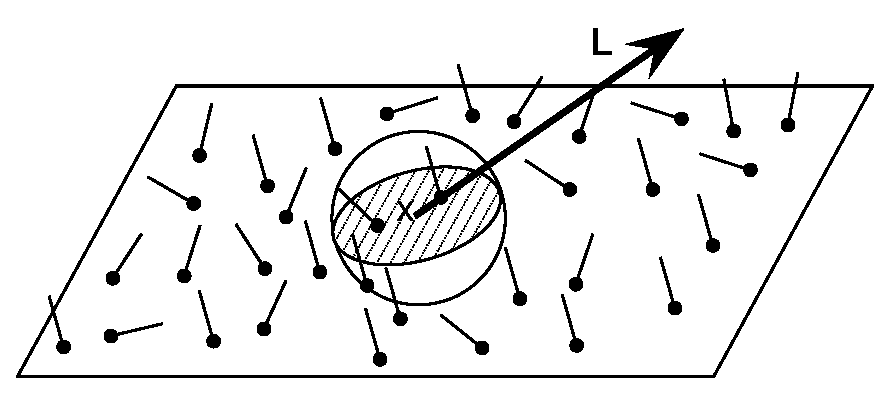
\includegraphics[width=.5\textwidth]{figures/pm/radiance-estimate}
	\caption{在光子映射技术中,非光泽表面上某个点的辐射亮度是通过使用它周围最近的一些光子进行估计的}
	\label{f:pm-sphere-estimate}
\end{figure}

式\ref{e:pm-approximated-radiance}仍然包含一个未知项$\triangle A$,它与$x$附近的光子密度有关,通过假设$x$附近的局部区域是平坦的,我们可以将包含$n$个光子的球体投影到这个平面上得到一个圆形区域,如图\ref{f:pm-sphere-estimate}所示:

\begin{equation}
	\triangle A=\pi r^{2}
\end{equation}

\noindent 这里$r$表示球体的半径,即$x$到所有选取的$n$个光子的最大距离,因此式\ref{e:pm-approximated-radiance}可以写为:

\begin{equation}\label{e:pm-approximated-radiance-area}
	L_r(x,\vec{\omega})\approx  \cfrac{1}{\pi r^{2}}\sum^{n}_{p=1}f_r(x,\vec{\omega}_p,\vec{\omega})\triangle\Phi_p(x,\vec{\omega}_p)
\end{equation}
 
\noindent 该估计是基于局部区域是平坦的这样的假设的,因此其估计的精度与参与估计的光子数量有关,因为我们使用了一个球体去定位参与估计的光子,这就可能会包含一些不满足这个假设的光子,例如物体边缘和角落都可能导致面积估计是错误的。直观上看,参与估计的光子数量越多,则式\ref{e:pm-approximated-radiance-area}就会变得更加精确,因为球体区域就会收缩得越来越小,光子越靠近$x$则辐射能量的估计越准确。在极限的情况下,我们可以得到如下结果: 

\begin{equation}\label{e:pm-photon-estimate-limit}
	\lim_{N\to\infty} \cfrac{1}{\pi r^{2}}\sum^{\lfloor N^{\alpha}\rfloor}_{p=1}f_r(x,\vec{\omega}_p,\vec{\omega})\triangle\Phi_p(x,\vec{\omega}_p)=L_r(x,\vec{\omega})\text{ for }\alpha\in ]0,1[
\end{equation}

\noindent 其中,$N$表示光子图中光子的总数量。对于所有(不包含脉冲函数的)BRDF反射函数,并且局部区域平坦的所有表面上的点,式\ref{e:pm-photon-estimate-limit}都是成立的。式\ref{e:pm-photon-estimate-limit}背后的逻辑是:首先,无限的光子数量$N$能够更准确地表述物体表面的辐射能量分布,因此方差逐步降低;其次,被选取参与估计的光子数量$N^{\alpha}$也是无限的,因此包含这些用于估计的光子的球体体积也将变得无限小,因此偏差也会逐步降低。

$\alpha$决定着式\ref{e:pm-photon-estimate-limit}中”极限“的程度,$N^{\alpha}$($\alpha\in]0,1[$)保证了参与估计的光子数量无限小于总的光子数量,并且它说明我们始终可以通过增加光子图中光子的数量来提高辐射亮度估计的精度。

\begin{figure}
\sidecaption
	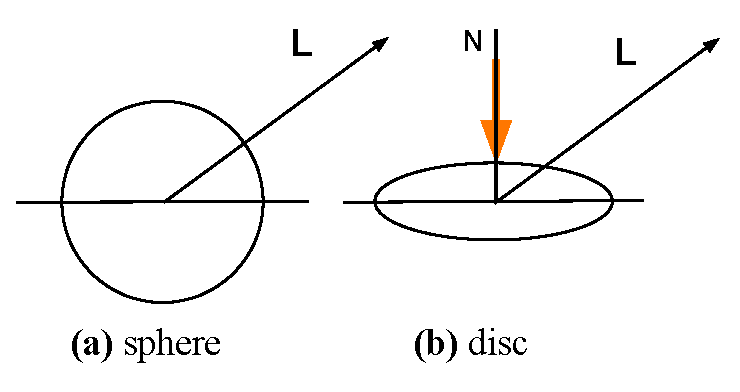
\includegraphics[width=.55\textwidth]{figures/pm/disc}
\caption{(a)使用球体搜索最近邻的光子,(b)使用垂直于表面法线的盘体或者椭球体搜索最近邻光子,它可以看做从法线反方向挤压球体形成,法线上的箭头表示挤压的方向}
\label{f:pm-sphere-and-disc}
\end{figure}

球体是一种比较简单的体积,可以很高效地计算到表面上的投影面积。在实践中也可以使用其他体积用于最近邻光子的搜索,此时式\ref{e:pm-approximated-radiance}中的$\triangle A$项应该替换为对于的面积,它应该是表面上经过$x$点的正切面与使用体积的相交面积部分。

例如一种更精确的体积是通过对球体沿表面$x$处的法线方向挤压形成的盘面(disc)或椭球体(ellipsoid),如图\ref{f:pm-sphere-and-disc}(b)所示。使用盘面的好处是可以减少对不在局部平面上光子的选取,例如墙角或者物体边缘处的光子。修改后的体积比较贴近于表面,例如它可以阻止墙表面上的光子进入门表面上位置的估计。但是盘面体积仍然不能阻止由于面积区域估计错误导致的问题,例如一个平面被一个垂直于该面的薄面分割,此时两边的辐射能量可能差别很大,但是两边的光子由于同处于一个平面而可能被放到一起进行估计,这样的问题可以通过后面介绍的过滤方法来减弱。





\subsection{渲~~染}\label{sec:pm-rendering}
光子映射技术并不是一个完整的全局光照解决方案,它主要是被设计用于加速蒙特卡洛光线追踪的计算,更具体地说,它仅处理间接漫反射光照以及焦散效果,而将光泽/镜面反射的光照计算留给光线追踪本身。

上述的说法其实并没有告诉到底应该怎样利用光子图进行光照计算,或者说光子图到底提供了什么信息,说它相对于完整的全局光照还缺乏什么。所以我们来首先梳理一下这些问题,它们对于后面渲染的过程的理解将很有帮助。




\subsubsection{光子图到底提供了什么信息}
光子图到底提供了什么信息呢,由第\ref{sec:pm-three-photon-maps}节的内容可知,焦散光子图包含的路径为:$LS^{+}D$,而全局光子图包含的路径为:$L\{S|D\}^{*}D$(这里暂时抛开体积内的光子路径),即是它包含了所有从光源出发终点为漫反射表面的路径。

那么相对于完整的全局光照:$L\{S|D\}^{*}E$,它还差什么信息呢。通过分析可以得出还缺少的路径为:$S^{*}E$,即缺少由摄像机发出的观察光线$E$,以及可能的最后一段或多段为连续镜面/光泽反射的路径,即$S^{*}E$。

上述的分析告诉了我们渲染阶段应该干什么:从摄像机发出观察光线,如果第一次相交的表面为漫反射面,则该光线的光照贡献可以直接通过光子图中的光子进行估计,包括全局光子图和焦散光子图(直接焦散),这能够渲染所有包括$L\{S|D\}^{*}DE$的路径;如果第一个相交的面为镜面或光泽面,则使用一般的光线追踪方法使用重要性采样发射新的光线,重复此步骤直到遇到漫反射面,此时和前一种情况一样处理,这能够渲染所有包括$L\{S|D\}^{*}DS^{+}E$的路径。

通常这样的方式,就可以结合光线追踪和光子图实现完全全局光照路径的渲染。并且可以看到,通过使用焦散光子图强制包含$LS^{+}D$路径,以及结合摄像机光线阶段对镜面和光泽面的处理,即$S^{*}E$路径,所以光子映射技术完全能够轻松处理$S^{+}DS^{+}$间接焦散路径。

最后需要注意的是,尽管上述的分析没有什么问题,但由于受光子数量的限制,来自光子密度估计形成的光照贡献并不是很精确,为了提高渲染质量,\cite{a:GlobalIlluminationusingPhotonMaps}在使用光子图的时候提出了区分两种不同的场景:精确计算和近似计算。精确计算用于那些直接对摄像机可见,或者从摄像机出发首先经历了(少数)几次镜面/光泽反射的顶点,此外它也包括那些从光线起点到交点的距离小于某个阈值的顶点,这样可以避免例如墙角处不精确的颜色渗透(color bleeding)\myindex{颜色渗透}{color bleeding};近似计算则适用于那些光线离开摄像机后已经经历过一次漫反射的交点,或者那些对像素值贡献很小的顶点。





\subsubsection{渲染通道}
通过上面的分析,在渲染阶段,我们还是使用一个传统的光线追踪的方式,由摄像机向场景中发射摄像机光线,这些光线在场景中传播并根据表面材质参数及光照情况返回该方向的辐射亮度值。唯一不同的是,当计算每个顶点处的漫反射光照贡献值时,我们直接从光子图中根据前面讨论的辐射亮度估计计算出该顶点出射方向的辐射亮度,而不是继续在该顶点半空间上对入射辐射亮度进行积分。

首先,BRDF反射函数可以根据粗糙度划分成两个部分:光泽/镜面反射率:$f_{r,s}$,以及漫反射率:$f_{r,d}$:

\begin{equation}
	f_r(x,\vec{\omega}^{'},\vec{\omega})=f_{r,s}(x,\vec{\omega}^{'},\vec{\omega})+f_{r,d}(x,\vec{\omega}^{'},\vec{\omega})
\end{equation}

\noindent 其次,在光子映射中,我们可以将光照的来源(即入射辐射亮度)划分成三个部分(可以看做三种不同类型的光源,所有路径最终当然光照贡献都来自它们):

\begin{itemize}
	\item $L_{i,l}(x,\vec{\omega}^{'})$,直接光照(direct illumination)\myindex{直接光照}{direct illumination},即直接接受来自真实光源的光照。
	\item $L_{i,c}(x,\vec{\omega}^{'})$,焦散光照,它们是从光源出发至少经过一次镜面/光泽面反射/折射后到达漫反射面的间接光照。
	\item $L_{i,d}(x,\vec{\omega}^{'})$,其他间接光照,它们是从光源出发至少经过一次漫反射后并落在漫反射表面的间接光照。
\end{itemize}

有了上述这些光照效果(或者路径类型\footnote{通常,我们可以根据路径类型来区分不同的光照效果。})分类,在光子映射技术中通常将反射方程划分成以下4个不同的组成部分,每个部分使用不同光照来源进行光照的计算:

\begin{equation}\label{e:pm-four-componenets-equation}
\begin{aligned}
	L_r(x,\vec{\omega})=&{\rm \int}_\Omega f_r(x,\vec{\omega}^{'},\vec{\omega}) L_{i,l}(x,\vec{\omega}^{'}) (\vec{\omega}^{'}\cdot\vec{n}) {\rm d}\vec{\omega}^{'}+ \\
	&{\rm \int}_\Omega f_{r,s}(x,\vec{\omega}^{'},\vec{\omega}) (L_{i,c}(x,\vec{\omega}^{'})+L_{i,d}(x,\vec{\omega}^{'})) (\vec{\omega}^{'}\cdot\vec{n}) {\rm d}\vec{\omega}^{'}+ \\
	&{\rm \int}_\Omega f_{r,d}(x,\vec{\omega}^{'},\vec{\omega}) L_{i,c}(x,\vec{\omega}^{'}) (\vec{\omega}^{'}\cdot\vec{n}) {\rm d}\vec{\omega}^{'}+ \\
	&{\rm \int}_\Omega f_{r,d}(x,\vec{\omega}^{'},\vec{\omega}) L_{i,d}(x,\vec{\omega}^{'}) (\vec{\omega}^{'}\cdot\vec{n}) {\rm d}\vec{\omega}^{'}
\end{aligned}
\end{equation}

\noindent 在上式中,第一部分表示直接光照,由于直接光照往往非常重要,精确计算(例如摄像机直接观察到的漫反射表面)需要使用传统光线追踪的方法,这可以参考第\ref{sec:pt-direct-illumination}节的内容;近似的计算(如需要计算两次反弹的漫反射光照)则可以直接从全局光照图中估计获取。

第二部分表示光泽/镜面反射,使用的是光照/镜面反射系数$f_{r,s}$,由于光泽反射的光照贡献值通常很大,所以它们通过传统的光线追踪方式进行计算,不涉及任何光子的估计。

第三部分表示焦散光照,它仅发生于漫反射表面,所以使用的反射系数是$f_{r,d}$,如果要求使用精确计算,则从焦散光子图中获取光子进行估计,如图\ref{sec:pm-rendering}(a)所示,否则从全局光子图中获取光子进行近似计算。

第四部分表面多次漫反射(multiple diffuse reflection)\myindex{多次漫反射}{multiple diffuse reflection},使用的反射系数是$f_{r,d}$,它表示入射光从离开光源之后已经至少经过了一次漫反射,然后又从当前漫反射表面反射出去,因此这部分的光照通常很柔和。实际的计算可以从漫反射表面根据BRDF分布采样得到一些方向,然后对来自这些方向的漫反射使用全局光子图进行估计,如图\ref{sec:pm-rendering}(b)所示。

\begin{figure}
	\sidecaption
	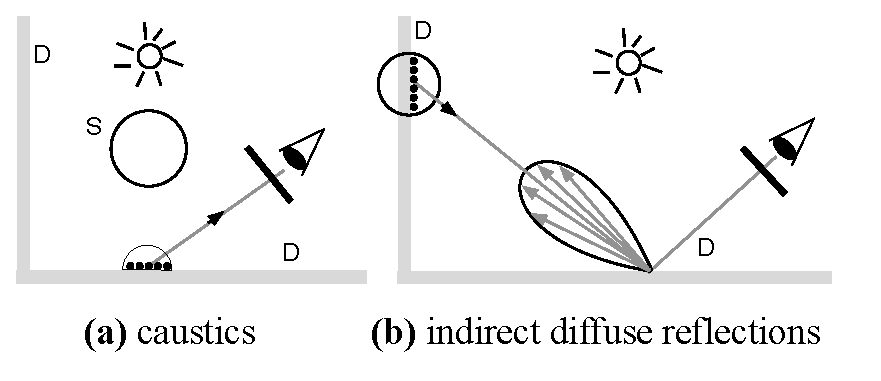
\includegraphics[width=0.65\textwidth]{figures/pm/rendering}
	\caption{(a)焦散效果渲染,和(b)多次漫反射。这也是光子映射技术非常擅长的两种效果(光照路径)}
	\label{f:pm-rendering}
\end{figure}







\section{渐进式光子映射}\label{sec:pm-progressive-pm}
基本的光子映射算法提出了一种高效实现焦散和间接漫反射等传统光线追踪技术比较难于(甚至不可能)实现的光线路径的有效方法,然而由于基本的光子映射技术需要存储整个场景的光子图,因此对于复杂的场景,处理器内存容量的大小限制了其所能达到的实际效果。

例如对于图\ref{f:pm-complex-caustics}所示的场景,这是一个包含大量焦散面的场景,因此整个场景的光子图需要非常高的密度才能避免比较明显的噪点,这时渲染的图像质量就很大程度上依赖于可用的内存大小。

\begin{figure}
\sidecaption
	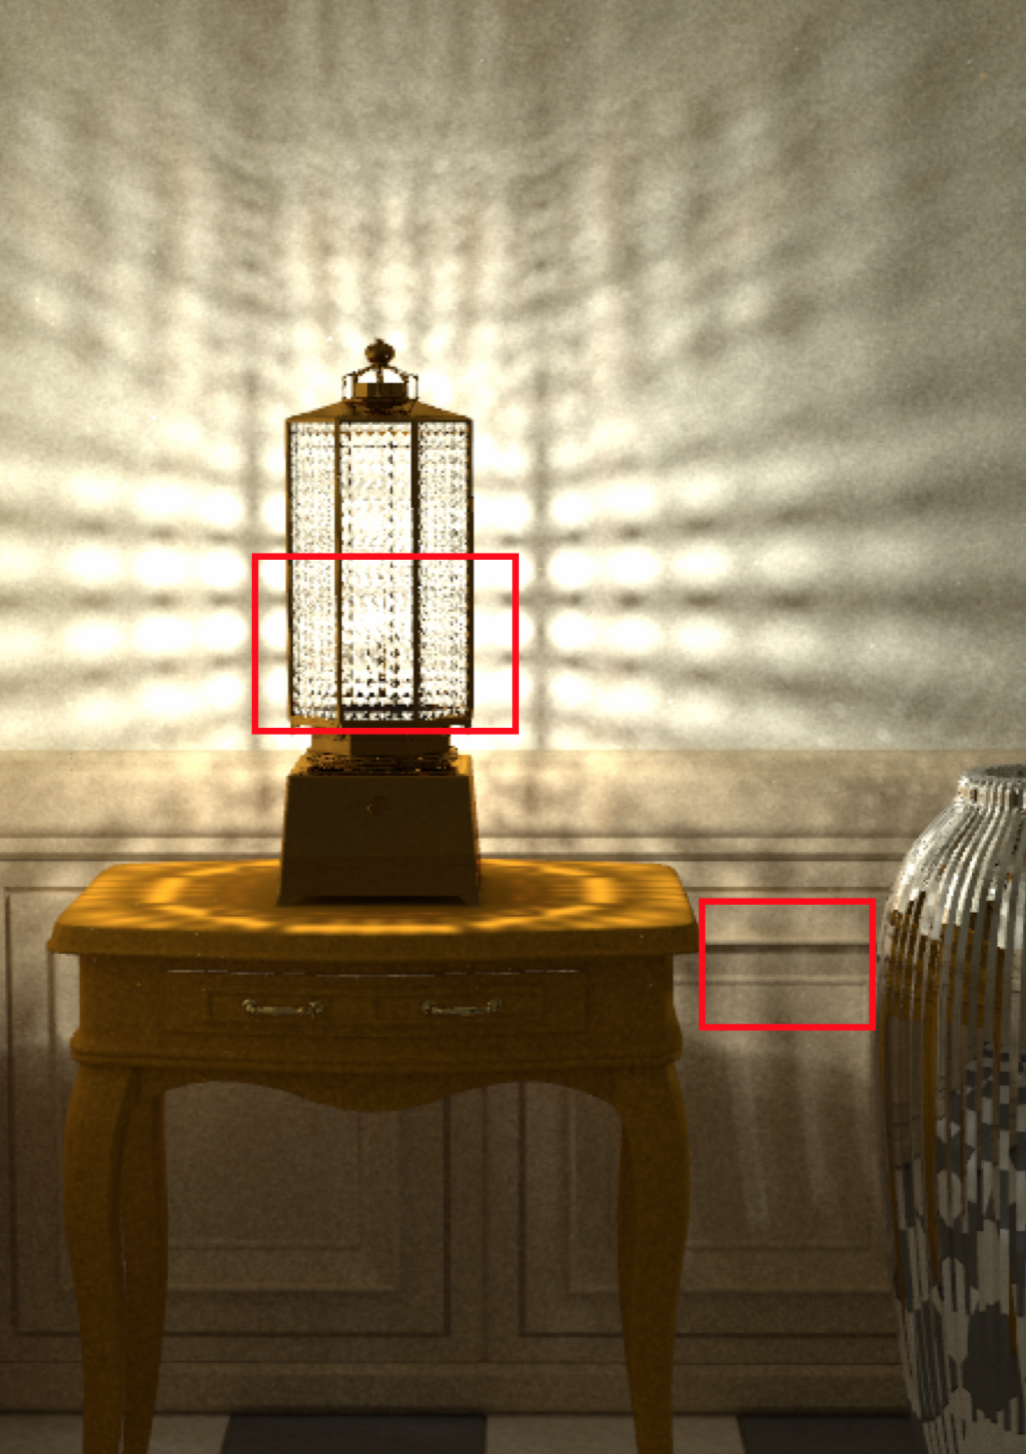
\includegraphics[width=.35\textwidth]{figures/pm/pm-21}
	\caption{一个包含复杂光照分布的场景:光源位于一个玻璃罩内部,光子从光源发出穿过玻璃罩照射在漫反射墙面上,产生非常复杂且面积较大的焦散分布及形状}
	\label{f:pm-complex-caustics}
\end{figure}

为了克服光子映射内存限制的问题,\cite{a:ProgressivePhotonMapping}提出了渐进式光子映射技术,它将光子追踪阶段分拆成多个迭代的过程,每个迭代阶段只需要存储其对应的少量光子,因此整个迭代过程就可以任意提高总的光子的数量,通过这样的分拆就可以在不需要一次性存储所有光子的情况下,模拟任意精度的光照传输计算。这同时也使得第\ref{sec:pm-three-photon-maps}讨论的对光子图的分类变得不再必要。

渐进式光子映射的主要原理是随着迭代步骤的增加,在提高参与估计的光子数量的同时,减少参与估计光子的体积(半径范围,或是过滤的带宽),并使得整个迭代的结果符合式\ref{e:pm-photon-estimate-limit}的结果。因此渐进式光子映射的主要内容是关于怎样以及以什么标准划分每个迭代过程。

第\ref{sec:pm-basic-ppm}将会介绍基本的渐进式光子映射;由于该算法依赖于存储所有摄像机路径样本,所以对于复杂的场景或者需要大量摄像机光线路径样本的效果(例如聚焦和运动模糊等),其精度仍然受内存大小的限制,第\ref{sec:pm-stochastic-ppm}节介绍的随机渐进式光子映射进一步解除了该限制;第\ref{sec:pm-error-estimation}节介绍的误差估计可以用于将渲染结果的误差控制在一定的阈值内;最后,第\ref{sec:pm-probabilistic-ppm}节将会从一种更简单的角度推导和理解渐进式光子映射的原理。





\subsection{基本渐进式光子映射}\label{sec:pm-basic-ppm}
首先回忆前面讨论的一般的光子密度估计:

\begin{equation}
	L(x,\vec{\omega})\approx \sum^{n}_{p=1} \cfrac{f_f(x,\vec{\omega},\vec{\omega}_p)\phi_p(x_p,\vec{\omega}_p)}{\pi r^{2}}
\end{equation}

\noindent 上述的估计假设$x$附近的局部区域是平坦的,因此参与该点辐射亮度估计的光子位于一个平坦的表面上。该估计也是光子映射算法偏差的来源,因为每个作为总的辐射亮度贡献值的其中一部分的光子能量被平滑了。

随着光子密度的增加,光子密度估计就会逐渐收敛至正确的结果(一致性),这要求光子图中光子的数量是无限的,同时参与估计的光子的数量也是无限的,并且覆盖参与估计光子的体积的半径应该逐渐收敛至0。

我们可以通过以下方式来满足上述的要求:对于具有数量为$N$的光子图,其中仅有$N^{\beta}$个光子($\beta\in[0,1]$)被用于每个位置的估计计算。在这种情况下,随着$N$逐步趋向于无限,$N^{\beta}$也会趋向于无限,但是$N^{\beta}$始终无限小于$N$,这样就保证了半径$r$会收敛至0,则极限情况下上式可以写为\cite{b:RealisticImageSynthesisUsingPhotonMapping}:

\begin{equation}\label{e:pm-consistent-equation}
	L(x,\vec{\omega})=\lim_{N\to\infty} \sum^{\lfloor N^{\beta} \rfloor}_{p=1} \cfrac{f_f(x,\vec{\omega},\vec{\omega}_p)\phi_p(x_p,\vec{\omega}_p)}{\pi r^{2}}
\end{equation}

\noindent 在标准的光子映射中,上述的结果只是理论上成立,因为无限数量的光子不可能被存储在内存中。但是渐进式光子映射则可以在不需要同时存储所有光子的情况下满足上式的要求。

\begin{figure}
	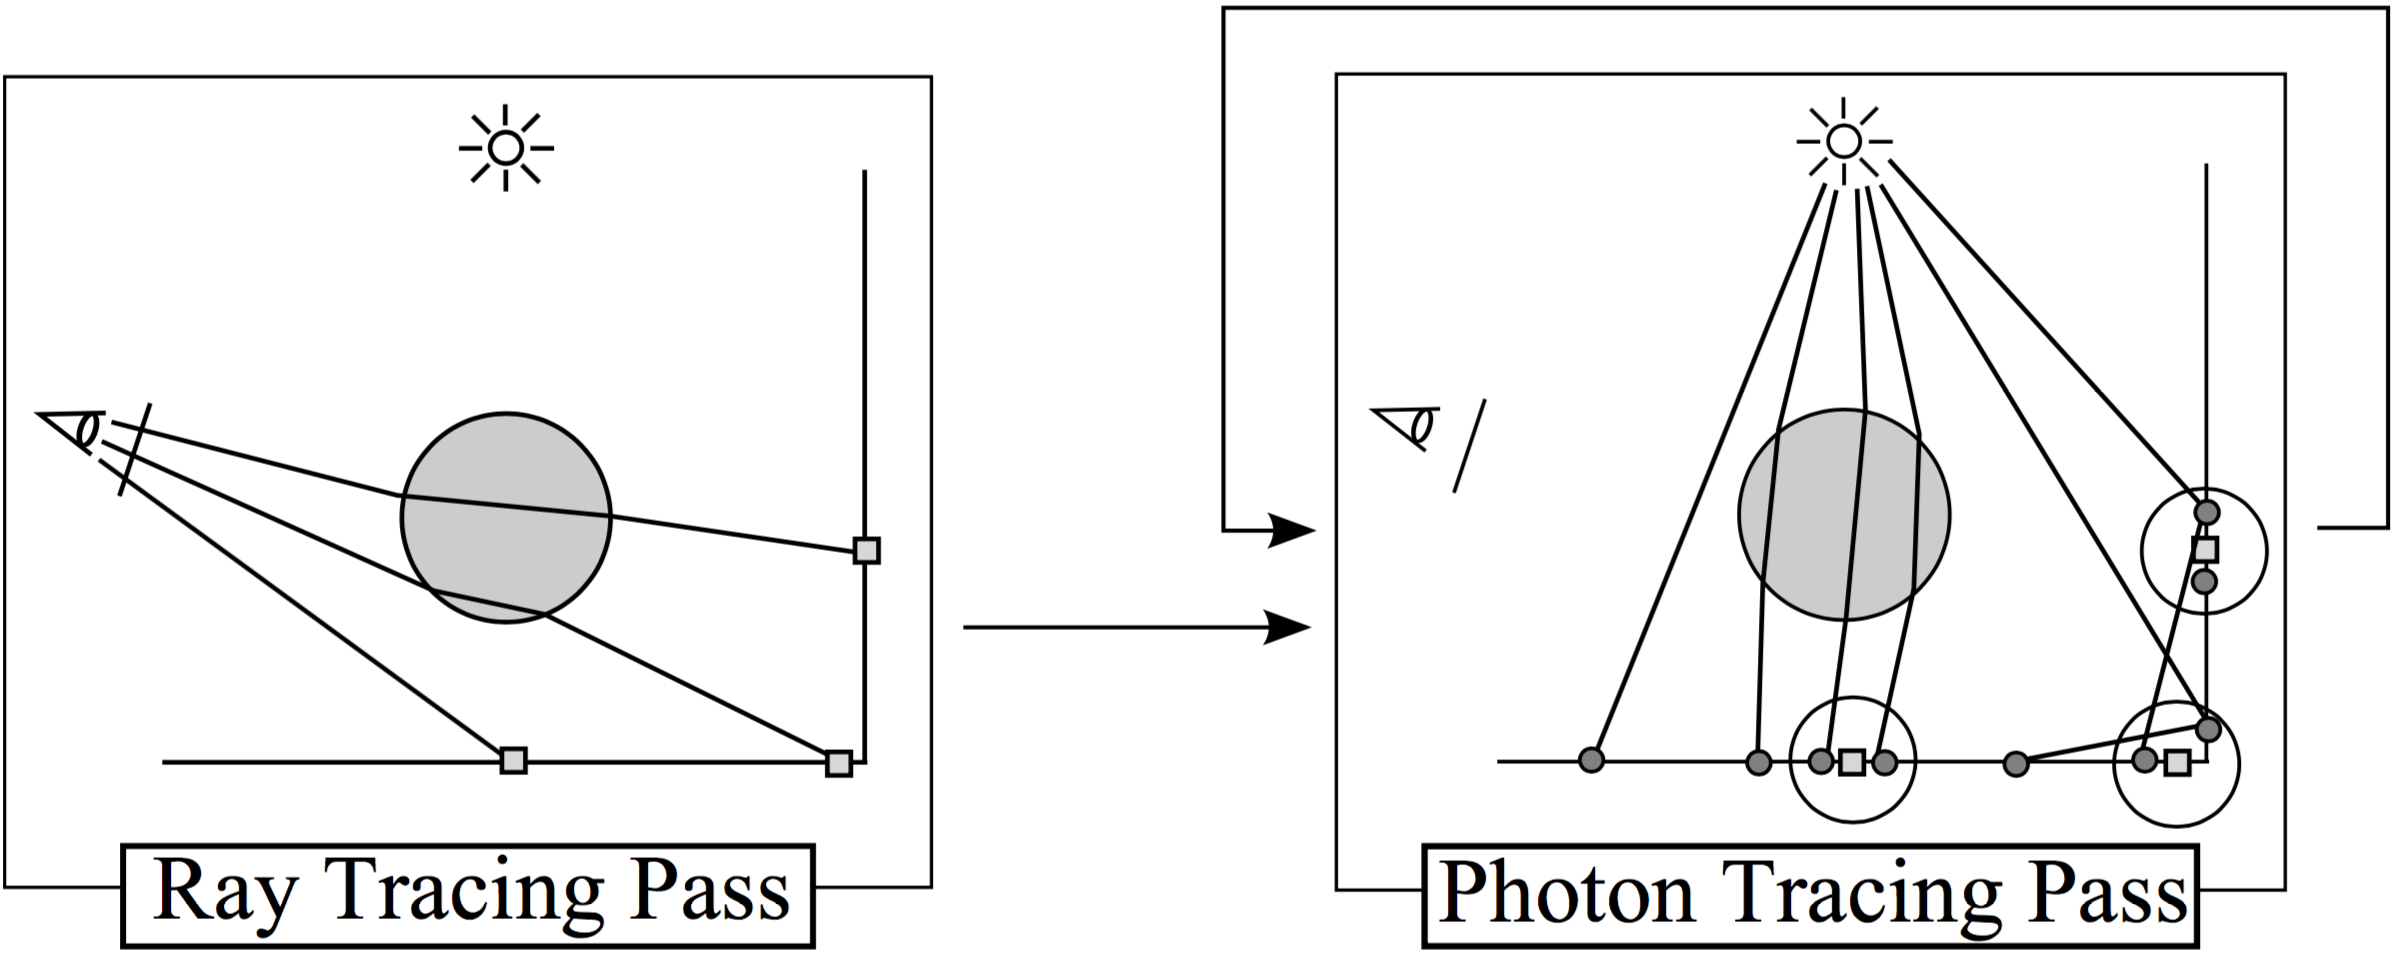
\includegraphics[width=\textwidth]{figures/pm/pm-18}
	\caption{渐进式光子追踪使用一个光线追踪通道,以及紧随着多个光子追踪通道}
	\label{f:pm-progressive-photon-mapping}
\end{figure}

渐进式光子映射(progressive photon mapping)\myindex{渐进式光子映射}{progressive photon mapping}是一种多通道(multi-pass)\myindex{多通道}{multi-pass}的方法,其中第一个通道为传统的光线追踪,如图\ref{f:pm-progressive-photon-mapping}左边小图所示,它从摄像机向场景发射出光线,此后光线在场景中传播直至遇到漫反射表面时停止并被记录;第二个通道为多个迭代的光子追踪通道,如图\ref{f:pm-progressive-photon-mapping}右边小图所示,在每个迭代中对前面光线追踪的每个记录点进行光子辐射亮度估计计算,每一个迭代都可以增加整个光照的精度,整个算法是渐进式的。




\subsubsection{光线追踪通道}
在传统的光子映射算法中,光子图首先在光子追踪通道被构建,然后在光线追踪阶段,光线从摄像机通过屏幕区域向场景发射出并传播,在漫反射表面停止并收集来自光子的光照,此过程称为最终聚集(final gather)\myindex{最终聚集}{final gather},同时在光子映射语境中,光线追踪通道的摄像机光线也称为最终聚集光线(final gather rays,FGRs)\myindex{最终聚集光线}{final gather rays}。

为了提高光子映射及最终聚集计算的计算效率,\cite{a:FastFinalGatheringviaReversePhotonMapping}提出了反转光子映射(reverse photon mapping)\myindex{反转光子映射}{reverse photon mapping}的概念,反转光子映射在第一个通道使用光线追踪,并把最终聚集光线在漫反射表面的交点,称为命中点(hit point)\myindex{命中点}{hit point},存储在一个特殊结构的k-d树\footnote{实际上是一个只有叶节点才会包含命中点的k-d树结构,且每个叶节点包含多个空间位置上相邻的命中点,这样可以加速对多个最近邻命中点的搜索。}中,然后在第二个阶段使用光子追踪。反转光子映射通过这样的方式提高最终聚集的性能:首先对光子图按空间排序(增加了内存访问的连贯性),然后遍历光子图中的每个光子,并搜索命中点k-d树中的kNN最近邻命中点以计算当前光子对该命中点的光照贡献。除了计算结构的修改,反转光子映射不涉及任何对基本光子映射算法的修改(例如近似计算等),因此它们渲染出的图像质量是完全一致的。

渐进式光子映射使用了和反转光子映射类似的思路,但是其目的不是为了提高最终聚集的计算性能,而是通过克服传统光子映射内存的瓶颈提高最终图像的精度。渐进式光子映射首先在第一个通道使用光线追踪方法找到所有能够被图像空间上每个像素直接看到的表面(点),即是那些所有从摄像机出发经过所有镜面/光泽反射直到达到第一个非光泽面的命中点。对于每一个光线路径,我们存储该路径上所有BRDF反射函数中包含非光泽面分量的命中点,每个命中点的数据结构如算法\ref{a:pm-progressive-hit-point}所示。

\begin{algorithm}
\begin{lstlisting}[language=C++, mathescape]
struct hitpoint {
	position $x$            //命中点位置
	normal $\vec{n}$              //命中点处的法线
	vector $\vec{\sigma}$              //光线方向
	integer $BRDF$             //BRDF反射函数索引
	float $x,y$               //像素位置
	color $wgt$               //该路径对像素贡献的权重
	float $R$               //当前光子密度估计的半径 
	integer $N$             //已经累加的光子数量 
	color $\tau$               //已经累加的辐射通量
}
\end{lstlisting}	
\caption{渐进式光子映射中光线追踪阶段生成的命中点的数据结构}
\label{a:pm-progressive-hit-point}
\end{algorithm}

在上述算法\ref{a:pm-progressive-hit-point}中,前面的变量为命中点本身的固有属性,用于计算该命中点对其所在路径贡献,最后的三个变量是用于进行渐进式光子密度估计的辅助属性,它们是一些统计量,我们将在下面一节讨论。

此外,从这里也可以看出,渐进式光子映射需要缓存大量的命中点,即摄像机路径采样。为了降低噪点,摄像机路径的样本甚至可能会远远多于光子的数量,因此这又形成了新的内存制约,第\ref{sec:pm-stochastic-ppm}介绍的内容将进一步消除命中点缓存导致的问题。






\subsubsection{光子追踪通道}
光子追踪通道被拆分成多个光子追踪的迭代过程,如图\ref{f:pm-progressive-photon-mapping}右边小图所示,每个迭代光子追踪通道生成一个标准的光子图,并被用于累积光子能量到光线追踪通道产生的命中点上:在每个光子追踪通道结束之后,对所有命中点进行遍历并查找光子图中一定半径范围内的最近邻光子进行估计计算。这个过程和传统的光子映射是相同的,除了命中点是预先而不是实时生成的。

每个迭代的新的光子追踪通道并不是单纯的累积光子能量到命中点上(否则这个传统的光子映射就没有区别了),而是被用于增强每个命中点的估计计算的精度,这通过下面介绍的半径缩减和辐射通量更正来实现,这也正是渐进式光子映射能够提高图像质量的原因。

一旦每个迭代光子追踪通道的光照贡献被计算,该通道产生的光子图将不会再被使用而将被全部丢弃,系统将重新使用一个新的光子追踪通道用于提高命中点估计的精度,这也是渐进式光子映射克服光子图内存限制的方法。





\paragraph{半径缩减}
如算法\ref{a:pm-progressive-hit-point}所示,每个命中点$x$的数据结构包含一个半径$R(x)$,以及该半径范围内参与光照估计的累积光子数量$N(x)$,我们的目标是在减少这个半径的同时增加其包含的累计光子数量,使得整个迭代过程满足式\ref{e:pm-consistent-equation}的要求。

假设一定数量的光子追踪通道已经被执行过,在命中点$x$附件半径为$R(x)$的范围内累积的光子数量为$N(x)$,如图\ref{f:pm-radius-reduction}左边小图所示,如果此时新增加一个光子追踪通道,该通道内在$x$附近半径为$R(x)$的范围内内发现的光子数量为$M(x)$,如图\ref{f:pm-radius-reduction}中间小图所示,将这$M(x)$新的光子加入之前的累积光子数量$N(x)$中,则得到新的光子密度估计$\hat{d}(x)$:

\begin{equation}\label{e:radius-reduction-1}
	\hat{d}(x)= \cfrac{N(x)+M(x)}{\pi R(x)^{2}}
\end{equation}

\noindent 由于我们需要在每次迭代中缩减估计半径$R(x)$,设减少的半径为$dR(x)$,如果我们假设在半径$R(x)$范围内的光子密度是一个常数,则我们可以计算出新的半径$\hat{R}(x)=R(x)-dR(x)$范围内的光子数量$\hat{N}(x)$为:

\begin{equation}\label{e:radius-reduction-2}
	\hat{N}(x)=\pi\hat{R}{x}^{2}\hat{d}(x)=\pi (R(x)-dR(x))^{2}\hat{d}(x)
\end{equation}

\noindent 为了满足式\ref{e:pm-consistent-equation}的要求,即每次迭代后对每个命中点参与估计的光子数量必须增加,这要求$\hat{N}(x)>N(x)$)。为了简便,这里增加一个参数$\alpha = (0, 1)$来控制每次迭代后的累积光子数量满足式\ref{e:pm-consistent-equation}的要求:

\begin{equation}\label{e:radius-reduction-3}
	\hat{N}(x)=N(x)+\alpha M(x)
\end{equation}

\noindent 上式说明每次迭代每个命中点增加了$\alpha M(x)$个光子参与估计,如图\ref{f:pm-radius-reduction}右边小图所示。综合式\ref{e:radius-reduction-1},\ref{e:radius-reduction-2}以及\ref{e:radius-reduction-3}可以计算出$dR(x)$的值,最终得到缩减后的半径$\hat{R}(x)$为:

\begin{equation}
	\hat{R}(x)=R(x)-dR(x)=R(x)\sqrt{ \cfrac{N(x)+\alpha M(x)}{N(x)+M(x)}}
\end{equation}

\noindent 上式中,每次迭代都是独立于各个命中点的,这使得该算法不需要对传统的光子追踪作出任何修改。参数$\alpha$是一个用户输入参数,我们将在本章后面的误差分析相关章节看到它对于收敛速度的影响。


\begin{figure}
	\begin{center}
		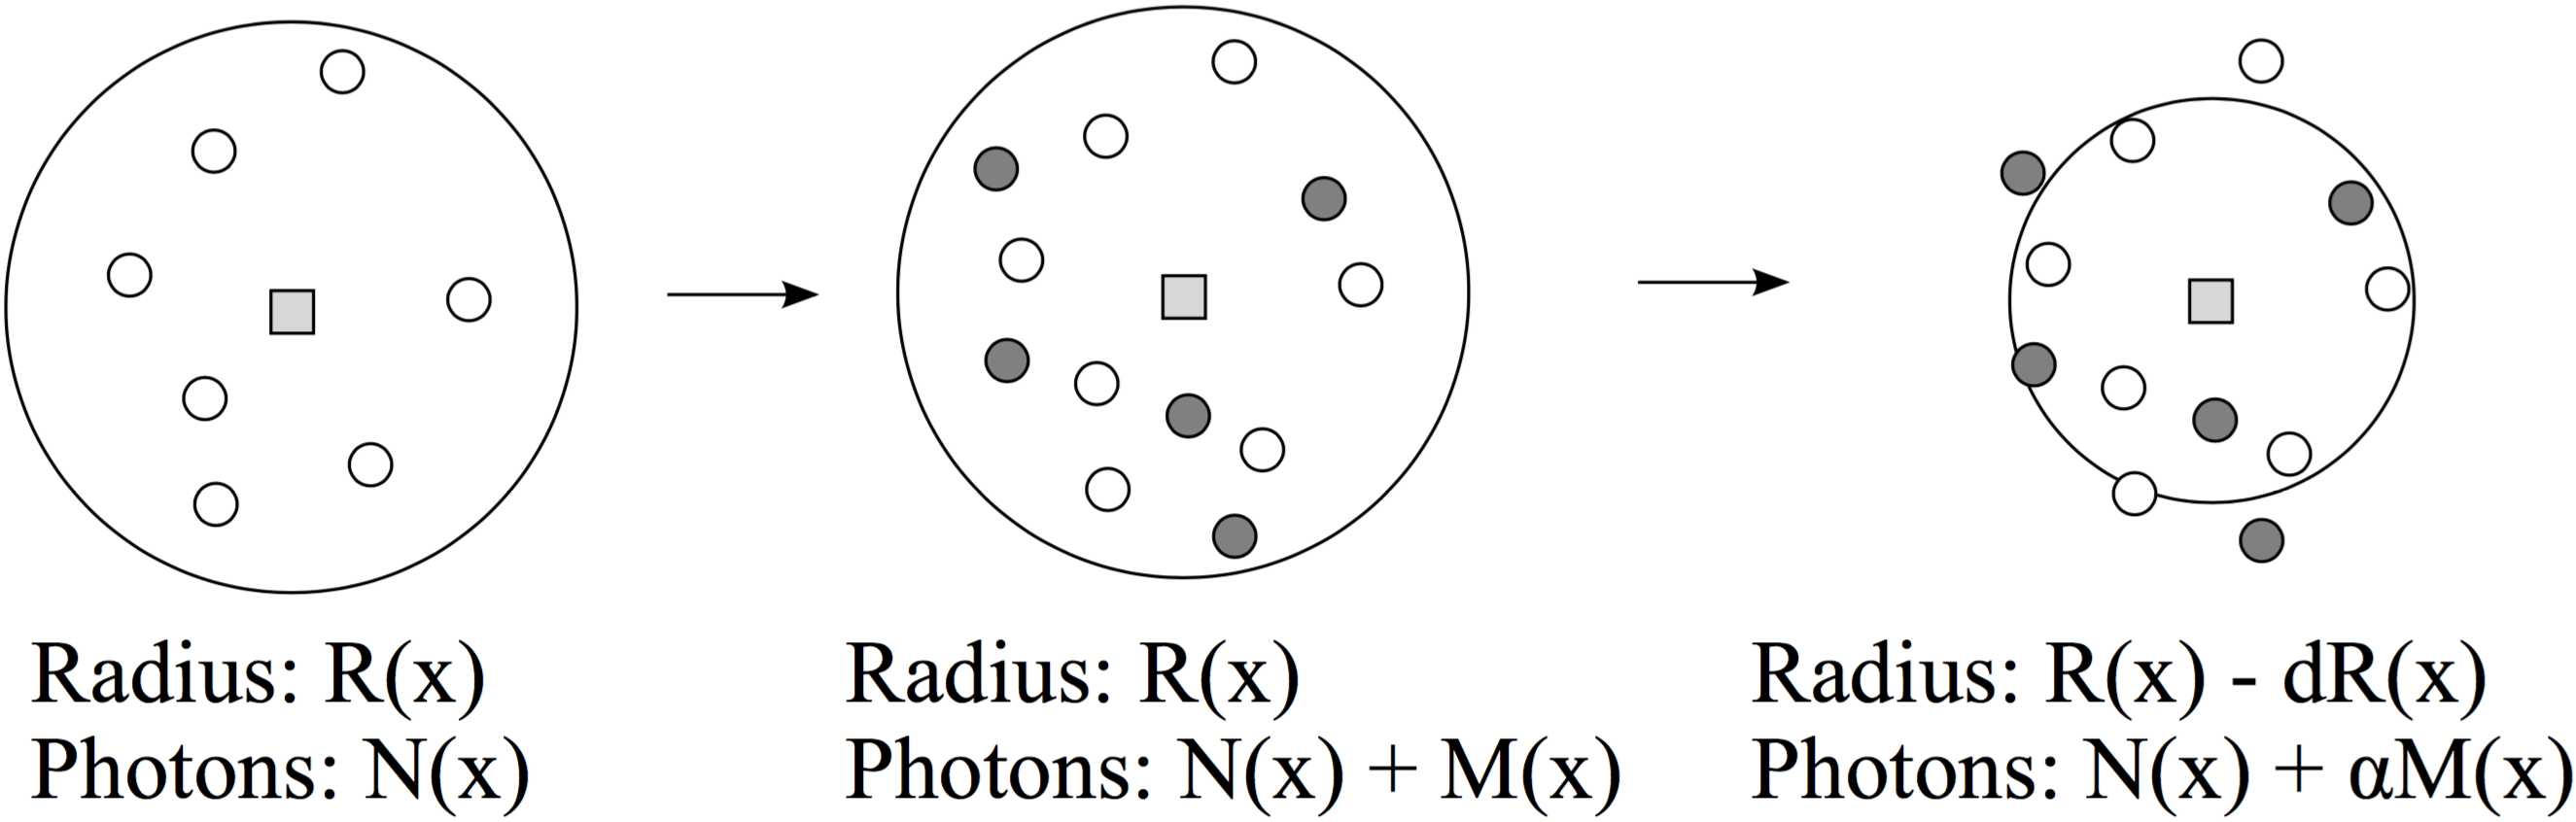
\includegraphics[width=\textwidth]{figures/pm/pm-19}
	\end{center}
	\caption{光线追踪通道产生的每个命中点被存储在一个全局的数据结构中,其包含一个半径以及一个累积光子能量变量;在每一次光子追踪通道之后,该半径内的新光子被加入,并根据新加入的光子缩减半径;渐进式光照亮度的估计能够保证每个命中点处的值最终收敛到正确的值}
	\label{f:pm-radius-reduction}
\end{figure}







\paragraph{辐射通量更正}
每个命中点在每次迭代中额外接收$M(x)$个光子,这需要被累积到总的辐射通量中,同时在这个累积的计算需要考虑半径缩减。每个命中点存储未经归一化的辐射通量总量,这个辐射通量来自每个光子与表面BRDF反射系数的乘积,记为$\tau(x,\vec{\omega})$:

\begin{equation}
\begin{aligned}
	\tau_N(x,\vec{\omega})&=\sum^{N(x)}_{p=1}f_r(x,\vec{\omega},\vec{\omega}_p)\phi^{'}_p(x_p,\vec{\omega}_p)\\
	\tau_M(x,\vec{\omega})&=\sum^{M(x)}_{p=1}f_r(x,\vec{\omega},\vec{\omega}_p)\phi^{'}_p(x_p,\vec{\omega}_p)
\end{aligned}
\end{equation}

\noindent 考虑到半径缩减,如图\ref{f:pm-radius-reduction}所示,假设$x$附近局部区域内的光照和光子密度是一个常数,可以得到下面经过调整的累积通量:

\begin{equation}
	\begin{aligned}
		\tau_{\hat{N}}(x,\vec{\omega})=&(\tau_N(x,\vec{\omega})+\tau_M(x,\vec{\omega})) \cfrac{\pi \hat{R}(x)^{2}}{\pi R(x)^{2}}\\
		=&\tau_{N+M}(x,\vec{\omega}) \cfrac{N(x)+\alpha M(x)}{N(x)+M(x)}
	\end{aligned}
\end{equation}

\noindent 其中,$\tau_{N+M}(x,\vec{\omega})=\tau_{N}(x,\vec{\omega})+\tau_{M}(x,\vec{\omega})$,这里$\tau_{\hat{N}}(x,\vec{\omega})$表示经过半径缩减后的累积通量,它对应于的光子数量为$\hat{N}(x)$。




\paragraph{辐射亮度计算}
在每次光子追踪通道之后,我们就可以\footnote{当然我们只需要在最后一次光子追踪通道之后计算一次辐射亮度,而每次迭代中只需要计算每个命中点缩减的半径$R$,累积光子数量$N$以及累积辐射通量$\tau$。}计算每个命中点的辐射亮度,这和标准的光子映射算法是类似的,只是这里需要使用经过缩减后的半径$R(x)$,以及经过调整的累积辐射通量$\tau (x,\vec{\omega})$(已经包含了BRDF预乘),新的辐射亮度估计公式为:

\begin{equation}
	\begin{aligned}
		L(x,\vec{\omega})&={\rm \int}_{2\pi}f_r(x,\vec{\omega},\vec{\omega}^{'})L(x,\vec{\omega}^{'})(\vec{n}\cdot\vec{\omega}^{'}){\rm d}\vec{\omega}^{'}\\
		&\approx  \cfrac{1}{\triangle A}\sum^{n}_{p=1}f_r(x,\vec{\omega},\vec{\omega}_p)\triangle\phi_p(x_p,\vec{\omega}_p)\\
		&= \cfrac{1}{\pi R(x)^{2}} \cfrac{\tau (x),\vec{\omega}}{N_{\rm emitted}}
	\end{aligned}
\end{equation}

上式中$N_{\rm emitted}$表示所有迭代中全部光子的数量\footnote{前面内容如式\ref{e:pm-radiance}并没有包含$N_{\rm emitted}$这个因子,这是因为那里的每个光子的能量都被归一化了,即$ \cfrac{\Phi}{N}$,但是本节使用的$\Phi$是没有被光子数量归一化的。这两者结果是一样的,但是渐进式光子追踪的文献通常在最后计算辐射亮度的时候进行归一化,为了便于参考文献,这里使用一致的表述。}。有了每个命中点的辐射亮度,就可以根据该命中点对应的像素坐标以及该命中点(摄像机路径)对应的采样权重,就可以计算其对应像素的光照贡献值。






\subsection{随机渐进式光子映射}\label{sec:pm-stochastic-ppm}
虽然渐进式光子映射能够收敛到正确的辐射亮度值,但是它被限制于只能计算一个固定(命中)点的值,这个属性限制了它的应用。在渲染中,我们常常需要计算围绕一个区域(而不是一个点)的辐射亮度。例如为了实现反走样,我们需要跟踪一个像素的足迹,计算该足迹范围内多条光线的(加权)平均值;对于景深(depth-of-field)效果,其处于景深范围内的场景成像比较清晰锐利,而景深外的场景则比较模糊,该部分每个像素点的值都是一个比较大的范围内辐射亮度的平均值;对于运动模糊,其需要计算移动物体在快门时间内的移动范围的平均值;此外,光泽反射/折射等都需要围绕一个区域进行计算。

上述这些效果都可以使用上一章介绍的分布式光线追踪(distributed ray tracing)\myindex{分布式光线追踪}{distributed ray tracing}来实现,在分布式光线追踪\cite{a:DistributedRayTracing}中,每个点的辐射亮度是该点法线方向半空间内多条光线的积分(这可以看做是对一个区域积分,而不是来自单个方向的反射/折射计算),如图\ref{f:pm-distributed-rt}所示。由于渐进式光子映射需要存储每个命中点的数据,因此对于处理这种分布式光线追踪效果,命中点的存储可能会超出处理器内存大小的限制。

\begin{figure}
	\sidecaption
	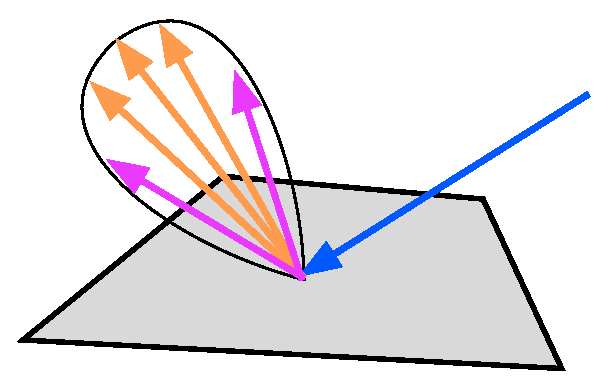
\includegraphics[width=0.4\textwidth]{figures/pm/distributed-rt}
	\caption{在分布式光线追踪中,每个点的辐射亮度值是来自于半空间上多条光线的积分,即可以看做是针对一个区域(而不是单个方向)的积分}
	\label{f:pm-distributed-rt}
\end{figure}

为了实现分布式光线追踪效果,\cite{a:StochasticProgressivePhotonMapping}提出了随机渐进式光子映射(stochastic progressive photon mapping,SPPM)\myindex{随机渐进式光子映射}{stochastic progressive photon mapping},它对渐进式光子映射做了一个非常简单的修改:相对于渐进式光子映射对每个命中点存储一组统计变量,来实现渐进式提高估计的精度,随机渐进式光子映射对一个固定区域$S$使用一组共享的统计变量,来实现渐进式提高该区域内平均辐射亮度估计精度的提高。为此,我们首先定义一个区域$S$内平均辐射亮度值为:

\begin{equation}
	L_i(S,\vec{\omega})= \cfrac{\tau_i(S,\vec{\omega})}{\pi R_i(S)^{2}N_e(i)}
\end{equation}

其中,$i$表示第$i$个光子追踪通道,$\tau_i(S,\vec{\omega})$表示区域$S$内的共享累积辐射通量,$R_i(S)$表示区域$S$内的一个共享半径。有了上式的表述,随机渐进式光子映射的主要内容便是证明上述的近似估计收敛至正确值,即:

\begin{equation}
	\lim_{i\to\infty}L_i(S,\vec{\omega})=L(S,\vec{\omega})
\end{equation}





\subsubsection{基本算法}
由于SPPM是基于PPM的一个简单扩展,这使我们可以在缺乏具体证明之前了解该算法的一些基本思路,因此本小节首先讨论SPPM的一些基本思路,下一节再做严谨的证明。

为了实现由基于(命中)点到基于区域的辐射亮度估计计算,SPPM对PPM做了两处修改:首先,它在每个光子追踪迭代之后抛弃现有的命中点,并使用一个新的分布式光线追踪通道产生一系列新的命中点,如图\ref{f:pm-stochastic-pmm}(b)所示;其次,它对于每个像素(而不是每个命中点)使用一组共享的统计变量,使得该像素对应的所有(分布式光线产生的)命中点共享这组统计变量,如图\ref{f:pm-stochastic-pmm}(c)所示。

\begin{figure}
\begin{fullwidth}
	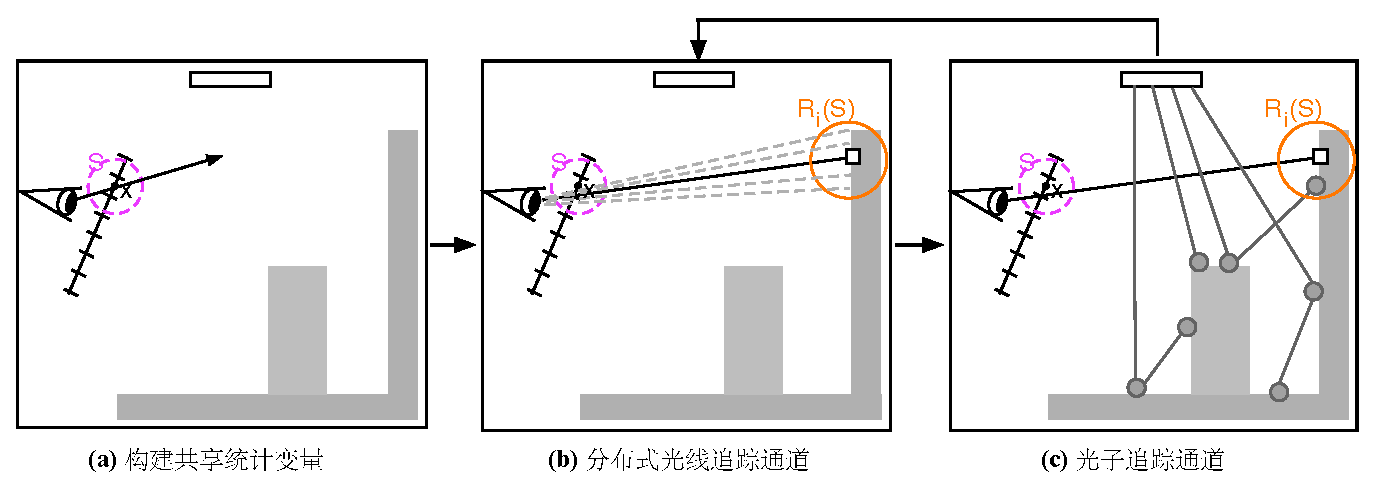
\includegraphics[width=1.0\thewidth]{figures/pm/sppm}
	\caption{与渐进式光子映射不同的是,为了计算一个区域内的平均辐射亮度值,SPPM中光子追踪通道(c)的命中点是由一个分布式光线追踪通道(b)随机产生的,并且每个命中点使用的统计变量由其所属像素对应的区域$S$决定,该区域(a)内的所有命中点共享一组统计变量}
	\label{f:pm-stochastic-pmm}
\end{fullwidth}
\end{figure}

上述的描述对于理解SPPM可能并不太直观,以下进一步使用SPPM算法的一般步骤对其进行描述。SPPM一般可以分为以下三个步骤,分别对应如图\ref{f:pm-stochastic-pmm}(a),(b)和(c),其中后两个步骤组成一个迭代的过程。

首先,对每个像素构建共享统计变量,如图\ref{f:pm-stochastic-pmm}(a)所示。SPPM的目标是计算一个区域$S$内的平均辐射亮度,在这个区域内,所有的命中点都共享一组统计变量,它们分别是:共享半径$R_i(S,\vec{\omega})$,共享光子数量$N_i(S)$,以及共享辐射通量$\tau_i(S,\vec{\omega})$,这里的下标$i$表示第$i$个迭代,一个像素的定义如算法\ref{a:pm-sppmpixel}所示。

\begin{algorithm}
\begin{lstlisting}[language=C++, mathescape]
struct SPPMPixel {
    Float radius = 0; //共享半径
    Float N = 0;      //共享累积光子数量
    Spectrum tau;     //共享累积辐射通量
    Spectrum Ld;      //直接光照贡献
    struct VisiblePoint {
        VisiblePoint() {}
        VisiblePoint(const Point3f &p, const Vector3f &wo, const BSDF *bsdf, const Spectrum &beta)
            : p(p), wo(wo), bsdf(bsdf), beta(beta) {}
        Point3f p;
        Vector3f wo;
        const BSDF *bsdf = nullptr;
        Spectrum beta;
    } vp;            //命中点
};
\end{lstlisting}	
\caption{\cite{b:pbrt}中SPPM实现单个像素的定义,每个像素包含一组共享统计变量,以及一个命中点(每次分布式光线追踪对每个像素产生一条摄像机光线)}
\label{a:pm-sppmpixel}
\end{algorithm}

上述这些统计变量和PPM中每个命中点的统计变量是相对应的,只是在SPPM中,$S$区域内的所有命中点共享一组统计变量。在每个迭代中它们使用和PPM类似的方式更新:

\begin{equation}\label{e:pm-shared-statistics}
\begin{aligned}
	N_{i+1}(S) &=N_i(S)+\alpha M_i(\vec{x}_i)\\
	R_{i+1}(S) &=R_i(S)\sqrt{ \cfrac{N_i(S)+\alpha M_i(\vec{x}_i)}{N_i(S)+M_i(\vec{x}_i)}}\\
	\Phi_i(\vec{x}_i,\vec{\omega})&=\sum^{M_i(\vec{x}_i)}_{p=1}f_r(\vec{x}_i,\vec{\omega},\vec{\omega}_p)\Phi_p(\vec{x}_p,\vec{\omega}_p)\\
	\tau_{i+1}(S,\vec{\omega})&=(\tau_{i}(S,\vec{\omega})+\Phi_i(\vec{x}_i,\vec{\omega})) \cfrac{R_{i+1}(S)^{2}}{R_i (S)^{2}}
\end{aligned}
\end{equation}

那么如何选择$S$呢?初学者在理解SPPM中的共享区域$S$的时候往往容易感到困惑,认为这个区域是固定于物体表面上的,然后落于该区域的命中点就使用其对应的共享统计变量。实际上SPPM中的区域$S$是针对一个像素而言的\footnote{当然这个说法并不准确,SPPM中的区域是针对所有需要使用分布式光线追踪来计算光照的那些点,这对于运动模糊以及景深来说其实就是图像空间上的像素;然而如果考虑光泽反射,此时的区域$S$还应该对应于所有光泽面上的点,如图\ref{f:pm-distributed-rt}所示。},通常每个像素对应一个区域,即每个像素包含一组共享变量,这个区域可以是一个像素大小,也可以包含相邻的多个像素(例如对于比较模糊区域,每个像素的值来自于周围多个像素范围内光照的混合),如图\ref{f:pm-stochastic-pmm}(a)中像素位置$x$处的区域$S$;然后所有为了计算该像素值而发出的摄像机光线产生的命中点都使用该像素对应的这组共享变量进行渐进式光子密度估计。所以这也和PPM有点区别:在PPM中从每个像素位置发出的摄像机光线一定是用于计算该像素的光照的,而在SPPM中从一个像素发射出的摄像机光线可能是用于计算相邻或附近像素的光照值的,这都由一些分布式光线追踪效果(如运动模糊,景深等)导致的结果。

其次,使用分布式光子追踪对每个像素生成命中点,如图\ref{f:pm-stochastic-pmm}(b)所示。通常在每个迭代每个像素只产生一条摄像机光线,为了实现分布式光子追踪效果,该光线的方向从该像素对应的区域$S$中随机采样生成,该光线在场景中传播遇到漫反射表面时停止产生一个命中点,如算法\ref{a:pm-sppmpixel}中的$vp$变量即表示该像素对应的命中点。由于每个命中点都与一个像素关联,因此在后续的概率密度估计中,该命中点使用的统计变量来自于第一步中构建的该像素的共享统计变量。当当前的迭代结束之后,所有的命中点被删除,在下一次迭代中重新生成新的命中点。这也便是SPPM打破命中点内存限制的关键:它将所有摄像机光线分拆到多个迭代中,每个迭代只需要存储和总的像素数量相等的命中点数据。

最后,使用光子追踪生成光子图并对命中点(所属的像素)进行估计,如图\ref{f:pm-stochastic-pmm}(c)所示。这和PPM中的光子追踪通道没有其他什么区别,唯一不同的是,式\ref{e:pm-shared-statistics}中的命中点$\vec{s}_i$的位置是由每次分布式光线追踪随机生成的,而不是像PPM中那样一个固定的命中点位置;光子追踪通道结束之后按式\ref{e:pm-shared-statistics}对每个命中点所属的像素的共享统计变量进行更新。

怎样验证SPPM是一致性的呢?原论文\cite{a:StochasticProgressivePhotonMapping}给出了相关的证明,然而这个证明过程相对比较复杂,这里不再讨论,我们要介绍的是另一种从概率的角度对上述算法思路一致性的证明方法,这种方法的思路更清晰,并且是后面即将讨论的适应性渐进式光子映射(第\ref{sec:pm-adaptive-ppm}节)的基础。





\subsection{渐进式光子映射的概率分析}\label{sec:pm-probabilistic-ppm}
在上一节中,通过对PPM的简单扩展,SPPM能够实现分布式光线追踪效果。\cite{a:StochasticProgressivePhotonMapping}通过使用和PPM类似的思路(例如围绕命中点针对辐射亮度估计进行分析)证明了SPPM的一致性,因此它也继承了PPM的一些属性,例如需要存储一组统计变量。

针对渐进式光子映射,\cite{a:ProgressivePhotonMappingAProbabilisticApproach}从概率的角度提出了另一种新的渐进式光子映射表述形式和研究方法,这种技术称为概率性渐进式光子映射(probabilistic progressive photon mapping)\myindex{概率性渐进式光子映射}{probabilistic progressive photon mapping}。相较于传统的(S)PPM,它围绕最终形态的像素值估计$\hat{I}_N$进行误差分析,推导出该估计满足一致性的条件,然后以此条件来验证渐进式光子映射的过程。由于它直接对像素值进行估计,因此天然包含了分布式光线追踪效果,并且它的结果不需要维护任何局部统计变量,可以以一种“盲目的”方式以一个固定的因子缩放估计的半径,因此各条摄像机光线是完全相互独立的,可以并行执行。

\begin{myshaded}
	这里的概率分析应该怎么理解呢?所谓的概率分析,即是使用概率论相关的知识进行求解分析,它使用随机过程来近似某个解(称为一个估计),并使用该随机过程的方差,期望等工具对估计的特征进行分析。
	
	在前面讨论的渐进式光子映射中,我们仅仅使用了概率密度估计的结果,并没有对该过程进行分析,并且后续的(共享)累积变量的处理完全是非概率的数值(近似)方法,所以它们不是概率分析的方法。
	
	本节将讨论的内容,它首先建立针对像素值建立的一个估计公式,然后后续所有的分析都围绕该估计使用方差,期望等概率工具对渐进式光子映射进行分析,所以这里使用的是概率分析方法。
\end{myshaded}

需要注意的是,本节讨论的内容和前面的(S)PPM算法的结果几乎是完全相同的,它可以看做是对渐进式光子映射算法的另(也是更简单的)一种诠释,它也有助于我们更好地理解PPM的思路。不过虽然其结果一致,但是由于概率性渐进式光子映射并不需要维护一组(共享)统计变量,因此其算法过程会有一些调整。




\subsubsection{基础条件}\label{sec:pm-ppm-basis}
如前面的内容可知,渐进式光子映射的思路是通过逐渐减小估计的半径,并同时增加参与估计的光子数量,来实现估计的方差和偏差逐渐消失的结果,及满足一致性。这涉及多个变量的控制,它使得迭代算法变得复杂,实践上我们希望通过少量的变量来控制整个渐进式收敛的过程(例如SPPM通过一个参数$\alpha$来控制半径缩小的速度即整个收敛的过程),这就需要找出这些变量之间的关系。

本节我们就通过概率的方法来寻找这些变量之间的关系。通过本章前面的内容可知,辐射亮度估计为:

\begin{equation}\label{e:pm-pixel-value}
	L(x,\omega)\approx \cfrac{1}{J}\sum^{J}_{j=1}k_r(x_j-x)\gamma_j
\end{equation}

其中,$J$表示该次迭代发射的光子总数,$\gamma_j$表示每个光子的光照贡献,$k_r$表示用于平滑的核函数。

针对该估计,我们希望通过概率的方法来分析各个变量之间的关系,即我们要分析上述估计的误差$\epsilon(x,r)$的一些特征,该误差定义为估计和真实值之间的差:

\begin{equation}\label{e:pm-ppm-error}
	\epsilon(x,r)= \cfrac{1}{J}\sum^{J}_{j=1}k_r(x_j-x)\gamma_j-L(x,\omega)
\end{equation}

首先我们来分析该估计的方差,即$Var[\epsilon (x,r)]$,假设核函数$k_r$范围内的光子概率密度为常数$p_i(x)$,并将光子光照值$\gamma_j$看做一个随机变量,\cite{a:ProgressivePhotonMappingAProbabilisticApproach}得处该方差可以近似为:

\begin{equation}
	Var[\epsilon(x,r)]\approx \cfrac{(Var[\gamma]+E[\gamma]^{2})p_l(x)}{Mr^{2}}{\rm \int}_{\mathcal{R}^{2}}k(\psi)^{2}{\rm d}\psi
\end{equation}

上式说明,辐射亮度估计的方差与发射的光子数量和估计的半径的平方成反比,给定一个期望的方差值$Var[epsilon]$,我们可以通过下式计算出对应的估计半径:

\begin{equation}
	r(x,Var[\epsilon])\approx\sqrt{ \cfrac{(Var[\gamma]+E[\gamma]^{2})p_l(x)}{MVar[\epsilon]}{\rm \int}_{\mathcal{R}^{2}}k(\psi)^{2}{\rm d}\psi}
\end{equation}

对于辐射亮度估计的偏差,$E[\epsilon (x,r)]$,\cite{a:ProgressivePhotonMappingAProbabilisticApproach}得出:

\begin{equation}
	E[\epsilon (x,r)]=r^{2}E[\gamma]\tau
\end{equation}

其中,$\tau$是一个常数我们将在第\ref{sec:pm-adaptive-ppm}节讨论。上式说明了辐射亮度估计的偏差与估计半径的平方成正比,因此随着半径的逐渐减小而消失。

本节的内容揭示了辐射亮度估计方差,偏差以及半径之间的关系,它们的结果将被用于后面的分析当中。



\subsubsection{光子映射的像素值估计形式}
光子映射和传统的光线追踪技术具有各自不同的光照传输表述形式,例如光子映射使用的辐射亮度估计,以及光线追踪使用的蒙特卡洛积分形式,传统的一些方法如\cite{a:AProgressiveErrorEstimationFrameworkforPhotonDensityEstimation}都是单独针对辐射亮度估计进行分析,此时为了分析分布式光线追踪效果,还需要额外做一些针对区域的方差和偏差的平均值计算,其分析过程相对比较复杂。

\cite{a:ProgressivePhotonMappingAProbabilisticApproach}首次将光子映射整合到蒙特卡洛积分形式中,然后通过统一的一个公式对光子映射进行分析,因此此种方法也称为概率方法(probabilistic approach)\myindex{概率方法}{probabilistic approach}。然而不同于无偏的路径追踪的是,辐射亮度估计引入了偏差,因此本节讨论的光子映射概率分析方法同时需要涉及偏差和方差的分析。

\begin{figure}
	\sidecaption
	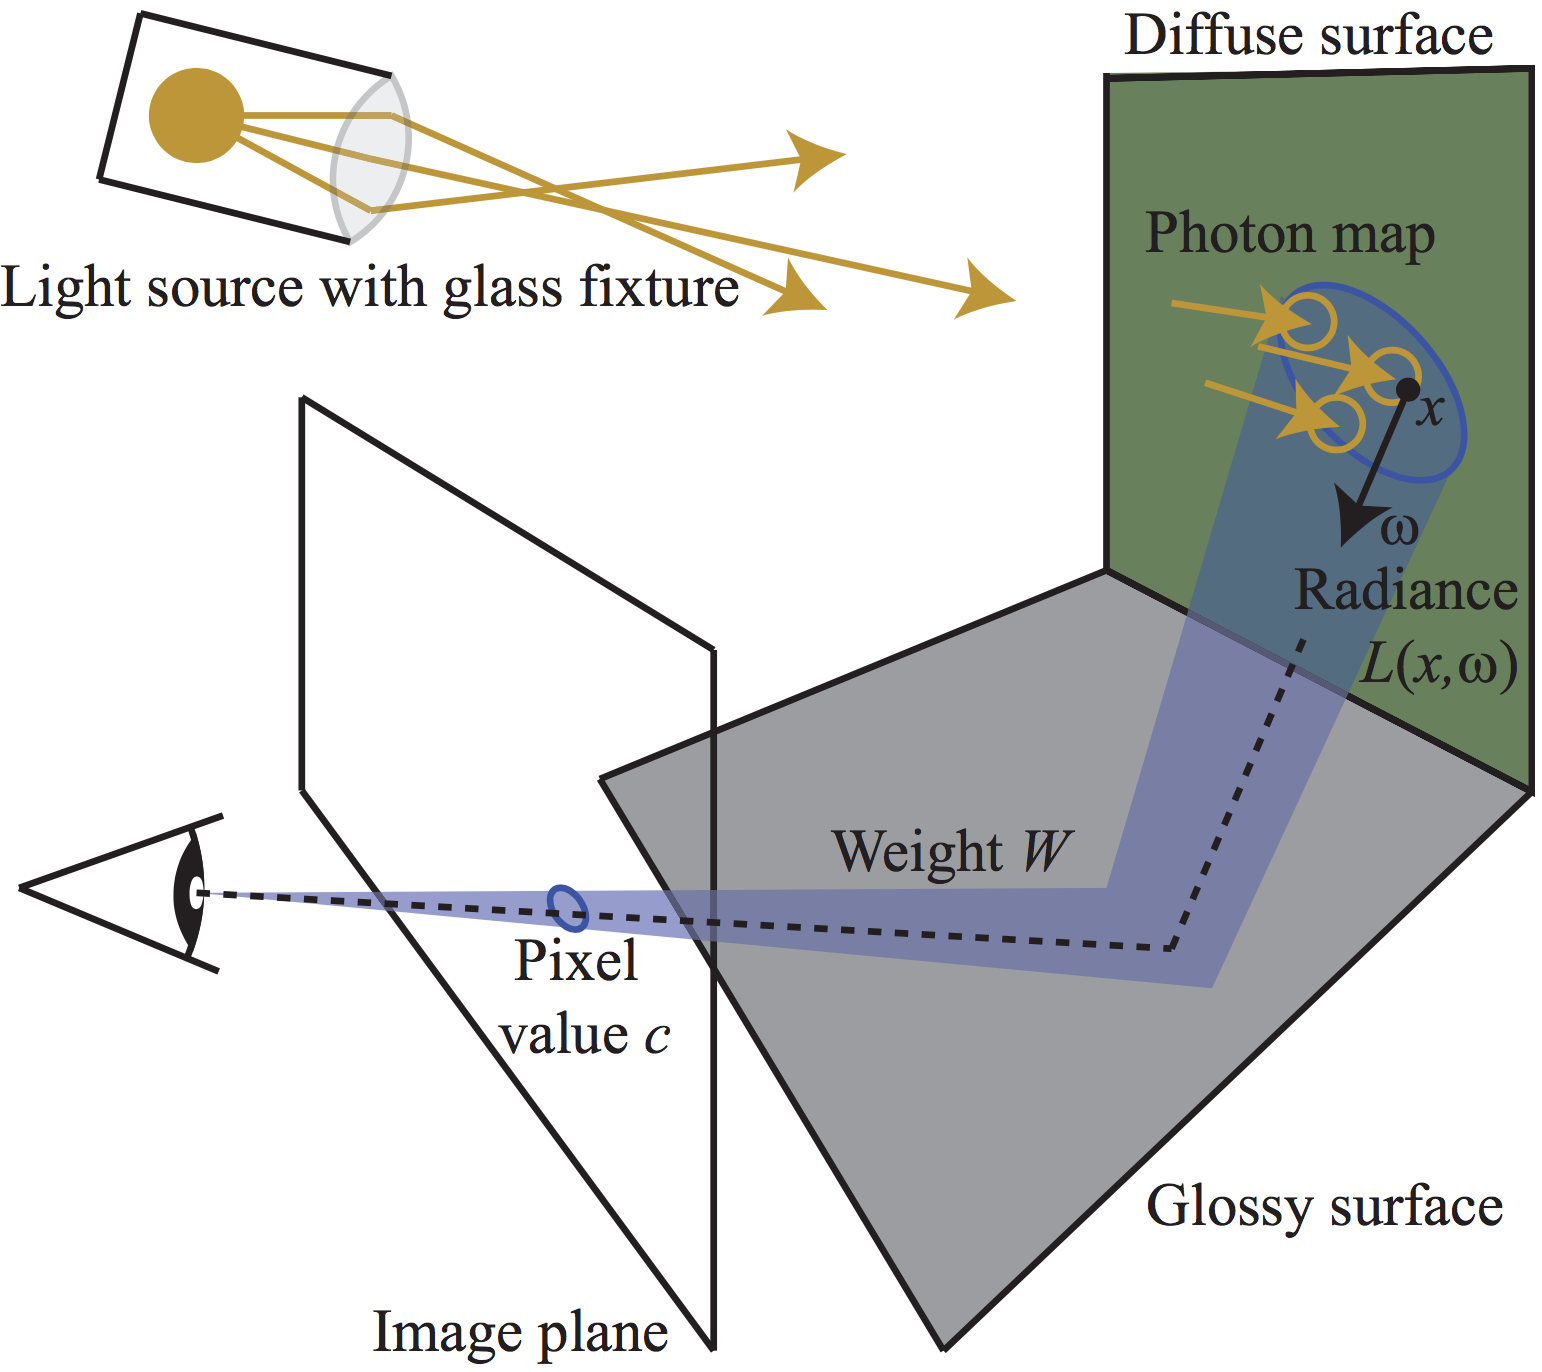
\includegraphics[width=0.6\textwidth]{figures/pm/pppm}
	\caption{一个基本的渐进式光子映射的场景,光源发出的光子经过一个玻璃罩面后击中漫反射表面生成光子图,然后摄像机光线从一个像素出发经过一系列光泽表面之后停留在漫反射表面,收集来自光子图的辐射亮度估计,像素值按照式\ref{e:pm-pixel-value}进行计算}
	\label{f:pm-pppm}
\end{figure}

通过上一章的内容可知,光照计算的目标是要计算一个像素值$I$:

\begin{equation}\label{e:pm-pixel-value}
	I={\rm \int} W(x,\omega)L(x,\omega){\rm d}x{\rm d}\omega
\end{equation}

\noindent 其中,$W(x,\omega)$是一个权重系数,它描述每个表面位置$x$处沿$\omega$方向的辐射亮度对像素值的贡献。这个权重可以包含用于反走样的像素过滤器,也可以包含一些分布式光线追踪效果,如运动模糊,景深,光泽反射等。我们通过发射摄像机光线来计算$W$,它包含了该光线到达漫反射点之前的所有(权重)系数的乘积,如图\ref{f:pm-pppm}所示。与路径追踪不同的是,式\ref{e:pm-pixel-value}中的辐射亮度$L(x,\omega)$来源于光子映射估计的结果,如图\ref{f:pm-pppm}所示。

为了便于分析,\cite{a:ProgressivePhotonMappingAProbabilisticApproach}使用$\hat{L}(x,\omega)=L(x,\omega)+\epsilon$来表述其估计的近似值,其中$L(x,\omega)$表示真实值,$\epsilon$表示由于光子密度估计而引入的误差,见式\ref{e:pm-ppm-error}。使用上述的模型,我们可以得到最终像素值的蒙特卡洛估计为:

\begin{equation}\label{e:pm-mc-ppm}
	\hat{I}_N= \cfrac{1}{N}\sum^{N}_{i=1} \cfrac{W_i}{p_{e,i}}(L(x_i,\omega_i)+\epsilon_i)
\end{equation}

\noindent 这里$\hat{I}_N$表示一个像素值的估计;由前面的内容可知,在SPPM的每个迭代中,每个像素发射一条摄像机光线并产生一个命中点,所以$N$表示从像素$c$发出的摄像机光线的样本数量,也即是渐进式光子映射中光子追踪通道迭代的次数;$p_e$则表示这些样本的概率密度函数。




\subsubsection{一致性条件}\label{sec:pm-pppm-convergence}
式\ref{e:pm-mc-ppm}表述的渐进式光子映射的一个比较重要的属性就是,它的每一个样本值都是使用一个新的光子分布(一个新生成的光子图)计算而得的,因此我们可以把$\epsilon_i$看做一个随机变量的一个样本,因为它依赖于随机分布的光子图。由此我们可以定义$N$个样本(或迭代)下的辐射亮度估计的平均误差:

\begin{equation}
	\bar{\epsilon}_N= \cfrac{1}{N}\sum^{N}_{i=1}\epsilon_i
\end{equation}

\noindent 由此可以分别得出该平均误差的方差和期望为:

\begin{equation}
\begin{aligned}
	Var[\bar{\epsilon}_N]&= \cfrac{1}{N^{2}}\sum^{N}_{i=1}Var[\epsilon_i]\\
	E[\bar{\epsilon}_N]&= \cfrac{1}{N}\sum^{N}_{i=1}E[\epsilon_i]
\end{aligned}
\end{equation}

我们的目标是获得一个满足一致性的估计$\hat{I}_N$:即随着样本数量$N$的增加,该估计的期望$E[\hat{I}_N]$收敛到正确值$I$,并且该估计的方差\footnote{为什么这里没有包含偏差$B[\hat{I}_N]$呢,如前所述,本节讨论的渐进式光子映射概率分析的其中一个假设是:每个摄像机光线样本对应的光子是独立同分布的,所以$\epsilon$可以看做一个随机数,但实际上$\epsilon_i$是受收缩半径$r_i$的影响而具有相关性的,下一节讨论的适应性渐进式光子映射将提供更加严谨的分析。}$Var[\hat{I}_N]$收敛至0。本章我们将证明,在什么样的条件下,式\ref{e:pm-mc-ppm}是满足一致性的,这样的条件将帮助建立下一节的渐进式光子映射算法。

首先来分析在什么条件下,式\ref{e:pm-mc-ppm}表述的估计其方差随着采样数量(或者迭代次数)$N$的增加收敛至0。$\hat{I}_N$的方差可以表述为:

\begin{equation}
\begin{aligned}
	Var[\hat{I}_N]&=Var\Biggl[ \cfrac{1}{N}\sum^{N}_{i=1} \cfrac{W}{p_e}(L+\epsilon_i) \Biggl]\\
	&= \cfrac{1}{N^{2}}\sum^{N}_{i=1}Var\Biggl[ \cfrac{W}{p_e}L \Biggl]+ \cfrac{1}{N^{2}}\sum^{N}_{i=1}Var\Biggl[ \cfrac{W}{p_e}\epsilon_i \Biggl]
\end{aligned}
\end{equation}

\noindent 上式中,第一项可以看做是传统的蒙特卡洛估计的方差,其按$1/N$的速度收敛至0,所以我们只需要考虑第二项。假设$W/p_e$和$\epsilon_i$是相互独立的,则第二项可以重写为:

\begin{equation}
\begin{aligned}
	 \cfrac{1}{N^{2}}\sum^{N}_{i=1}Var\Biggl[ \cfrac{W}{p_e}\epsilon_i \Biggl]=&Var\Biggl[ \cfrac{W}{p_e}\Biggl] \cfrac{1}{N^{2}}\sum^{N}_{i+1}Var[\epsilon_i]+E\Biggl[ \cfrac{W}{p_e}\Biggl]^{2} \cfrac{1}{N^{2}}\sum^{N}_{i+1}Var[\epsilon_i]\\
	&+Var\Biggl[ \cfrac{W}{p_e}\Biggl] \cfrac{1}{N^{2}}\sum^{N}_{i+1}E[\epsilon_i]^{2}
\end{aligned}
\end{equation}

\noindent 在上式中,$[ \cfrac{W}{p_e}]^{2}$可以看做常数,由于渐进式光子映射是一致性的,所以$E[\epsilon_i]\leq E[\epsilon_1]$,因此$\sum^{N}_{i+1}E[\epsilon_i]^{2}$是一个有限的常数,同样排除蒙特卡洛估计项,剩下其他项在满足以下条件时会随着$N\to\infty$而消失:

\begin{equation}
	 \cfrac{1}{N^{2}}\sum^{N}_{i=1}Var[\epsilon_i]=Var[\bar{\epsilon}_N]\to 0
\end{equation}

剩下还需要分析在什么条件下,式\ref{e:pm-mc-ppm}表述的估计其期望随着采样数量(或者迭代次数)$N$的增加收敛至真实值$I$。$\hat{I}_N$的期望可以表述为:

\begin{equation}
\begin{aligned}
	E[\hat{I}_N]&=E\Biggl[  \cfrac{1}{N}\sum^{N}_{i=1} \cfrac{W}{p_e}(L+\epsilon_i) \Biggl]\\
	&= \cfrac{1}{N}\sum^{N}_{i=1}E\Biggl[ \cfrac{W}{p_e}L\Biggl]+  \cfrac{1}{N}\sum^{N}_{i=1}E\Biggl[ \cfrac{W}{p_e}\Biggl]E[\epsilon_i]\\
	&I+E\Biggl[ \cfrac{W}{p_e}\Biggl] \cfrac{1}{N}\sum^{N}_{i=1}E[\epsilon_i]
\end{aligned}
\end{equation}

\noindent 上式使用了蒙特卡洛估计的期望等于其真实值的特性,所以要使$E[\hat{I}_N]=I$,必须随着$N\to\infty$时:

\begin{equation}
	 \cfrac{1}{N}\sum^{N}_{i=1}E[\epsilon_i]=E[\bar{\epsilon}_N]\to 0
\end{equation}





\subsubsection{实现收敛}
至此,我们推导出了实现式\ref{e:pm-mc-ppm}表述的估计满足一致性的条件,即使辐射亮度估计的平均误差$\bar{\epsilon}_N$的方差和期望在极限情况下同时收敛至零:

\begin{equation}\label{e:pm-consistent}
	\begin{aligned}
		Var[\bar{\epsilon}_N]\to 0 &\Rightarrow Var[\hat{I}_N]\to 0\\
		E[\bar{\epsilon}_N]\to 0 &\Rightarrow E[\hat{I}_N]\to I
	\end{aligned}
\end{equation}

同基本的渐进式光子映射一样,\cite{a:ProgressivePhotonMappingAProbabilisticApproach}也使用了一个参数来控制辐射亮度估计的方差:

\begin{equation}
	 \cfrac{Var[\epsilon_{i+1}]}{Var[\epsilon_i]}= \cfrac{i+1}{i+\alpha}
\end{equation}

\noindent 其中,$\alpha$为一个常数,并且满足$0<\alpha<1$。参数$\alpha$控制着在每个迭代中方差增加的速度。由此可以得出第$i$次迭代其方差与第一次迭代的关系为:

\begin{equation}
	Var[\epsilon_i]=Var[\epsilon_1]\Biggl(\prod^{i-1}_{k=1} \cfrac{k}{k+\alpha}\Biggl) i
\end{equation}

\noindent 进一步可以得出$N$次迭代其平均误差的方差为:

\begin{equation}
	Var[\bar{\epsilon}_N]= \cfrac{Var[\epsilon_1]}{N^{2}}\Biggl( 1+\sum^{N}_{i=2}\Biggl(\prod^{i-1}_{k=2} \cfrac{k}{k+\alpha}\Biggl) i\Biggl)
\end{equation}

通过使用后面第\ref{sec:pm-adaptive-ppm}会讨论的渐进分析可以得出$Var[\bar{\epsilon}_N]$随着$N$的逐渐增加而消失,并且其消失的速度为$\mathcal{O}(1/N^{\alpha})$。所以参数$\alpha$满足了式\ref{e:pm-consistent}的第一个条件。

对于式\ref{e:pm-consistent}第二个条件,由第\ref{sec:pm-ppm-basis}节的内容可知$E[\epsilon]$跟估计半径的平方$r^{2}$成正比,而$Var[\epsilon]$又与$r^{2}$成反比,因此我们可以得出$r$和参数$\alpha$之间的关系为:

\begin{equation}\label{e:pm-pppm-radius}
	 \cfrac{r^{2}_{i+1}}{r^{2}_i}= \cfrac{Var[\epsilon_i]}{Var[\epsilon_{i+1}]}= \cfrac{i+\alpha}{i+1}
\end{equation}

\noindent 因此可以得出辐射亮度平均误差的期望为:

\begin{equation}
	E[\bar{\epsilon}_N]= \cfrac{E[\epsilon_1]}{N}\Biggl( 1+\sum^{N}_{i=2}\Biggl(\prod^{i-1}_{k=2} \cfrac{k+\alpha}{k}\Biggl)  \cfrac{1}{i}\Biggl)
\end{equation}

同样,根据渐进分析可以得出上式随着$N$的增加而消失,其消失的速度为$\mathcal{O}(1/N^{1-\alpha})$。

通过上述的分析,我们看到可以使用一个参数$0<\alpha<1$使辐射亮度估计的平均误差的方差和偏差同时消失,即满足式\ref{e:pm-consistent-equation}一致的条件(式\ref{e:pm-consistent})。





\subsubsection{算法描述}\label{sec:pm-ppppm-algorithm}
我们已经讨论了怎样通过概率分析的方法来解释和验证渐进式光子映射。在上述的分析中,不再需要对每个命中点或每个像素区域记录一些(共享)累积变量,整个过程只需要一个控制方差变换的变量$\alpha$。因此,新的算法对内容的依赖进一步减少,并且各个迭代之间相互独立,可以并行进行。

算法\ref{a:pm-pppm}给出了基于概率分析的渐进式光子映射的算法的伪代码:

\begin{algorithm}
\begin{lstlisting}[language=C++]
i = 0
while (t < t_{\max}) {   //迭代的终止条件为时间
	生成光子图
	for all pixels {
		对每个像素发射一条摄像机光线直到击中漫反射表面
		记录命中点的位置,方向
		计算权重系数W
		生成路径的概率密度
		通过估计半径和迭代次数的关系计算当前迭代的半径
		计算辐射亮度估计
		更新像素值  
	}
	i = i + 1;
}
\end{lstlisting}	
\caption{基于概率分析的渐进式光子映射算法的伪代码,这里不再需要存储一些局部的累积变量,算法结构更加简单,并且各个迭代之间可以并行执行}
\label{a:pm-pppm}
\end{algorithm}

在算法\ref{a:pm-pppm}中,第2行的终止条件也可以改为使用像素值估计的方差$Var[\hat{I}_N]$小于某个给定阈值,这可以通过渐进分析计算得出,换句话说,我们可以预测在经过$N$次迭代之后输出像素值的方差;第9行的半径是根据式\ref{e:pm-pppm-radius}推导而出,它可以通过初始半径$r_1$和唯一的参数$\alpha$共同计算而出,也因此该算法不需要存储任何统计变量。

上述算法只包含两个用户参数:决定着整个估计的收敛速度的$\alpha$,以及任意的初始半径$r_1$,然后每次迭代的估计半径可以通过这两个参数直接计算而出,因此不再需要传统渐进式光子映射使用的累积变量。我们将在下一节进一步讨论这些参数对估计的影响,以及怎样选择最优化的参数。





\subsection{适应性渐进式光子映射}\label{sec:pm-adaptive-ppm}
在渐进式光子映射中,光子密度估计的半径$r_N$,或者称为核函数带宽(kernel bandwidth)\myindex{核函数带宽}{kernel bandwidth},是影响核估计效率的重要参数,它决定着核估计方差与偏差之间的平衡。在传统的渐进式光子映射\cite{a:ProgressivePhotonMapping,a:ProgressivePhotonMappingAProbabilisticApproach}中,估计半径呈指数式收缩:

\begin{equation}
	r^{2}_{N+1}=r^{2}_{N} \cfrac{N+\alpha}{N+1}
\end{equation}

其中,$N$表示迭代次数,$0<\alpha<1$。\cite{a:AdaptiveProgressivePhotonMapping}进一步将其简化为一个可以直接计算的公式:

\begin{equation}\label{e:pm-radius}
	r_N=r_{1}N^{ \cfrac{\alpha-1}{2}}\propto O(N^{ \cfrac{\alpha-1}{2}})
\end{equation}

之前的方法并没有对收缩系数$\alpha$和初始半径$r_1$作出比较明确的说明和选择,这两个参数却对估计有很重要的影响。如图\ref{f:pm-parameters}表示传统的渐进式光子映射在不同参数选择下的渲染结果及与参考结果的差异,首先图\ref{f:pm-parameters}(b)使用了较大的初始半径($k=50$)以及较小的收缩系数($\alpha=0.5$),较大的半径导致了较大的偏差,例如焦散面被过度平滑而与参考结果呈现较大的差异,同时又由于过快的半径收缩使得噪点也过早出现;图\ref{f:pm-parameters}(a)减小了初始半径,因此减小了偏差,但是过小的估计半径以及过快的收缩速度使得噪点比较严重;同样,对于图\ref{f:pm-parameters}(d),过大的初始半径以及过慢的收缩速度导致过大的偏差;对于图\ref{f:pm-parameters}(c),太小的初始半径导致较多的噪点,并且由于收缩速度过慢而过早出现偏差。

\begin{figure}
\begin{fullwidth}
	\includegraphics[width=1.0\thewidth]{figures/pm/parameters}
	\caption{使用传统的渐进式光子映射在不同的参数选择下的渲染结果比较(k表示使用k-NN来决定初始估计半径$r_1$的光子数量),每图的左上图表示经过少量迭代之后的渲染结果,右下图表示该渲染结果和参考结果的差异(图片来自\cite{a:AdaptiveProgressivePhotonMapping})}	
	\label{f:pm-parameters}
\end{fullwidth}
\end{figure}

本节,我们将以更严谨的理论分析这些参数的意义,以及怎样选择最合适的参数来使得估计的收敛速度最快,并且在有限的样本数量下,估计的均方差最小。





\subsubsection{渐进收敛速度}
参数$\alpha$控制着带宽$r_N$的收缩,因此控制着整个(而不是特定光子数量的)估计的方差与偏差的平衡,本节首先从渐进分析的角度,聚焦于最优$\alpha$参数的选择。

图\ref{f:pm-alpha}展示了对渐进式光子映射的渐进分析,这些数据来源于传统PPM渲染的结果,从图中可以看出,参数$\alpha$控制着像素值估计的收敛速率(即曲线的斜率,见左下角的小图),这个收敛速率是和初始带宽$r_1$无关的,注意这里初始的均方差值都是相同的,但是这里只截取了末端的部分。

\begin{figure}
	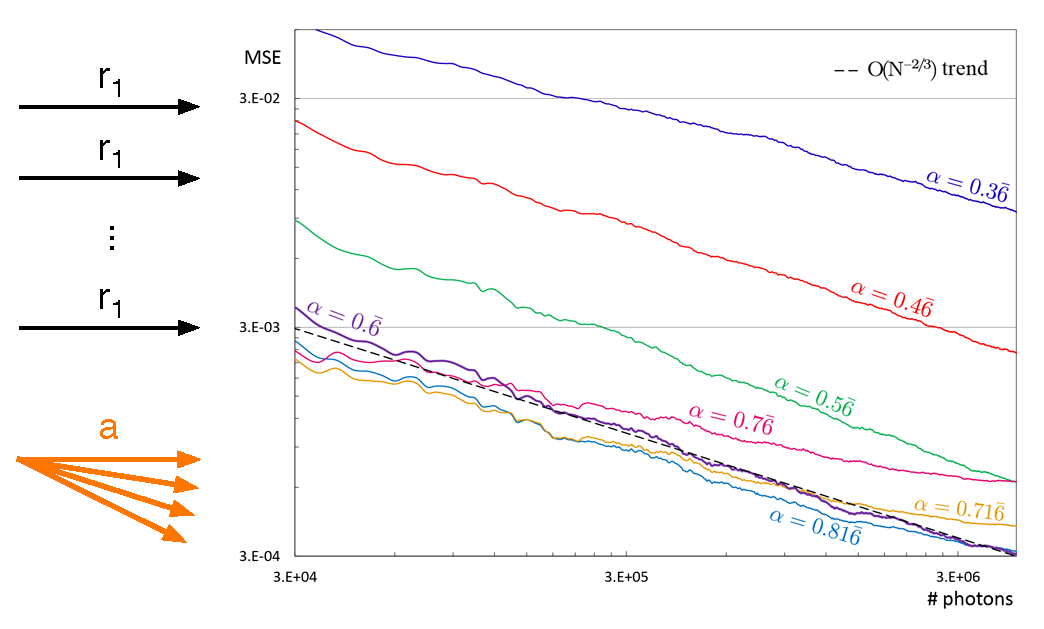
\includegraphics[width=1.\textwidth]{figures/pm/alpha}
	\caption{不同$\alpha$参数对误差收敛速度的影响,这里横轴为光子数量,纵轴为像素估计值的均方差,所有估计都使用相同的初始带宽$r_1$;从图中可以看出$\alpha$影响着曲线的斜率,而参数$r_1$影响着初始的误差值(图片素材来自\cite{a:AdaptiveProgressivePhotonMapping})}
	\label{f:pm-alpha}
\end{figure}

如前面的内容可知,估计的方差和偏差都是与$\alpha$参数有关的,因此如果直接求出像素值估计的均方差,由于均方差的收敛是与初始带宽无关的,那么应该可以从均方差的一些渐进属性当中得出一个最优的$\alpha$,它使得均方差的值最小。图\ref{f:pm-opt-a}展示了这种关系,它包含一个最小值,这就是我们要求的最优$\alpha$值。

\begin{figure}
	\sidecaption
	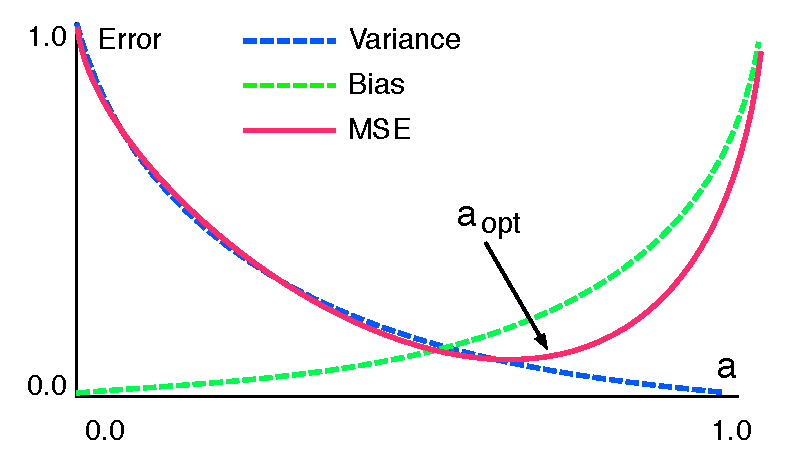
\includegraphics[width=0.55\textwidth]{figures/pm/opt-a}
	\caption{渐进式光子映射均方差和$\alpha$参数的关系,注意这里是和初始带宽$r_1$无关的,最小值就对应着最优的$\alpha$值}
	\label{f:pm-opt-a}
\end{figure}

我们首先需要推导出渐进式光子映射估计的渐进均方差(asymptotic mean squared error,AMSE)\myindex{渐进均方差}{asymptotic mean squared error},它由方差$Var[\hat{I}_N]$和偏差$B[\hat{I}_N]$的平方组成,其中方差由两个来源:即发射摄像机光线产生的方差以及核估计产生的方差,这里由于核估计产生的方差远远小于摄像机光线产生的方差,所以可以忽略不计,而偏差主要是来源于辐射亮度估计,综合前面的一些知识,可以得出AMSE的近似值为:

\begin{equation}\label{e:pm-mse}
\begin{aligned}
	AMSE[\hat{I}_N]&=Var[\hat{I}_N]+B[\hat{I}_N]^{2}\\
	&\approx \cfrac{1}{N}Var[ \cfrac{W}{p_e}L]+E\Biggl[ \cfrac{W}{p_e}\Biggl]^{2}\Biggl( \cfrac{Var[\epsilon_1]}{(2-\alpha)N^{\alpha}}+ \cfrac{E[\epsilon_1]^{2}}{\alpha^{2}N^{2-2\alpha}}\Biggl)
\end{aligned}
\end{equation}

然后对上式针对$\alpha$进行求导并令其值等于0来求图\ref{f:pm-opt-a}均方差曲线的最小值,得:

\begin{equation}
	N^{3\alpha-2}= \cfrac{\alpha^{2}Var[\epsilon_1]}{2(2-\alpha)E[\epsilon_1]^{2}}
\end{equation}

在上式中,右边的项是一个有限的值,而$N$是一个无限的值,所以要使等式成立,则可以得到最优的$\alpha$值为:

\begin{equation}
	\alpha_{opt}=2/3
\end{equation}

如果我们把该最优$\alpha$值代入式\ref{e:pm-radius},得到最优的带宽收缩率为:

\begin{equation}
	r_N=r_1N^{-1/6}\propto O(N^{-1/6})
\end{equation}

这也是一般统计学中渐进分析中的最优收缩率。

如果把最优$\alpha$参数值代入前面的方差和偏差的表述中,可以得到相同的收敛速度$O(N^{-2/3})$,因此$\alpha_{opt}$使得总的均方差MSE的收敛速度最快,任何其他非$\alpha_{opt}$值都会导致方差和偏差不一致的收敛速度,因此整个均方差的收敛速度减慢。





\paragraph{收敛性分析}
通过将最优收缩率$\alpha_{opt}$代入式\ref{e:pm-mse}可以得到渐进式光子映射的最优收敛速率为:

\begin{equation}
	AMSE[\hat{I}_N]\propto O(N^{-2/3})
\end{equation}

我们来比较一下渐进式光子映射和传统蒙特卡洛估计的收敛速度,由于蒙特卡洛估计是无偏的,因此均方差只包含方差项,即:$AMSE[MC]=Var[MC]\propto O(M^{-1})$,这里$M$表示每个像素对应的全路径采样的数量。由于PPM的收敛速度为$O(N^{-2/3})$因此比蒙特卡洛估计的收敛速度要慢,这是因为在PPM中构造一条全路径(从光源到摄像机)的概率同时还正比于估计面积$\pi r^{2}_N$,其收敛速度为$O(N^{-1/3})$,因此减小了全路径构造的概率。

然而这并不意味着我们应该总是采样无偏的蒙特卡洛估计,尽管蒙特卡洛估计具有更快的收敛速度,但是它包含较大的方差,其产生的噪点需要无限的路径采样才能消除,而有偏的光子映射利用偏差来换取方差的降低,因此可以在有效样本下实现更好的结果;其次,正确本章开头所描述,例如SDS路径等效果对于蒙特卡洛方法几乎是完全无能为力的。






\subsubsection{适应性带宽选择}
上述我们从像素值估计的均方差$AMSE[\hat{I}_N]$与收缩系数$\alpha$之间的关系出发,推导出了渐进式光子映射的最优收缩系数$\alpha_{opt}$,然而上述最优的$\alpha_{opt}$仅定义了在无限光子数量下带宽的收缩速率,很显然我们更关心的是有限的光子数量或迭代下的最优结果,即特定迭代次数下最小的均方差值,例如在图\ref{f:pm-alpha}中,初始带宽$r_1$的不同会导致特定光子数量下均方差呈现较大的差异,尽管它们可能具有相同的收缩速率,因此初始带宽$r_1$对特定迭代次数(或光子数量)下的均方差具有更重要的影响。

其次,目前我们讨论的渐进式光子映射的初始带宽$r_1$都是全局的,即对所有像素使用相同的初始带宽,由于具有相同的收缩速率$\alpha$,因此所有像素在每次迭代也都使用相同的带宽$r_N$,这显然不是最优的结果,例如对那些稀疏的区域应该使用较大的带宽以减小方差,而那些频率变化较大的边缘区域,则应该使用较小的带宽以减低偏差,因此带宽应该具有局部适应性。

不适当的初始带宽会使得迭代估计不断积累次优(suboptimal)的结果,例如对于过小的初始带宽,后续的所有带宽$r_N$都是根据收缩率$\alpha$计算出来的,因此最优的带宽不会被自动调整过来,因此导致每次迭代贡献很小,所以即使在很大的采样数量$N$下也可能保留较大的误差。

综上所述,局部带宽的选择非常重要,它严重地影响着有限迭代次数下的渲染质量(尽管极限情况下的收缩速度并不会发生变化),使在有限的迭代次数下能够达到更快的收敛速度,以下我们就将从像素估计的均方差$AMSE[\hat{I}_N]$与带宽$r_N$的关系出发,讨论一种带宽自适应的方法。





\paragraph{渐进式光子映射的路径空间公式}
核估计的带宽控制着其估计方差和偏差之间的平衡,因此为了选择最优(均方差最小)的核估计带宽,我们需要知道估计均方差和带宽之间的关系。\cite{a:AProgressiveErrorEstimationFrameworkforPhotonDensityEstimation}第一次针对辐射亮度估计的误差作出了分析,它围绕固定的命中点给出了其估计的误差和偏差与带宽的关系,然而该误差分析的结果对分布式光线追踪效果是无效的,为了更全面的对渐进式光子映射的误差进行分析,\cite{a:AdaptiveProgressivePhotonMapping}将辐射亮度估计整合到像素值计算当中,形成一个统一的路径空间的回归形式,因此能够完全的分析渐进式光子映射的误差行为。

不同于其他的渐进式光子映射算法,\cite{a:AdaptiveProgressivePhotonMapping}将光子映射算法表述为基于路径空间的像素值的局部回归形式:

\begin{equation}
	\hat{I}_N= \cfrac{1}{NJ}\sum^{N}_{i=1}\sum^{J}_{j=1}k_{r_i}(\mathbf{e}_i-\mathbf{l}^{i}_j)\psi_{i,j}
\end{equation}

这里$N$表示摄像机路径的数量(或者迭代的次数),$J$表示每次迭代中发射的总的光子数量,即光源路径的数量,$\psi_{i,j}$表示一条全路径的光照贡献,每条全路径由一条摄像机路径的尾点$\mathbf{e}_i$与一条光源路径的尾点$\mathbf{l}^{i}_{j}$相连,该条全路径的权重被一个核函数$k_{r_i}$相乘,如图\ref{f:pm-path-space}所示。

\begin{figure}
	\sidecaption
	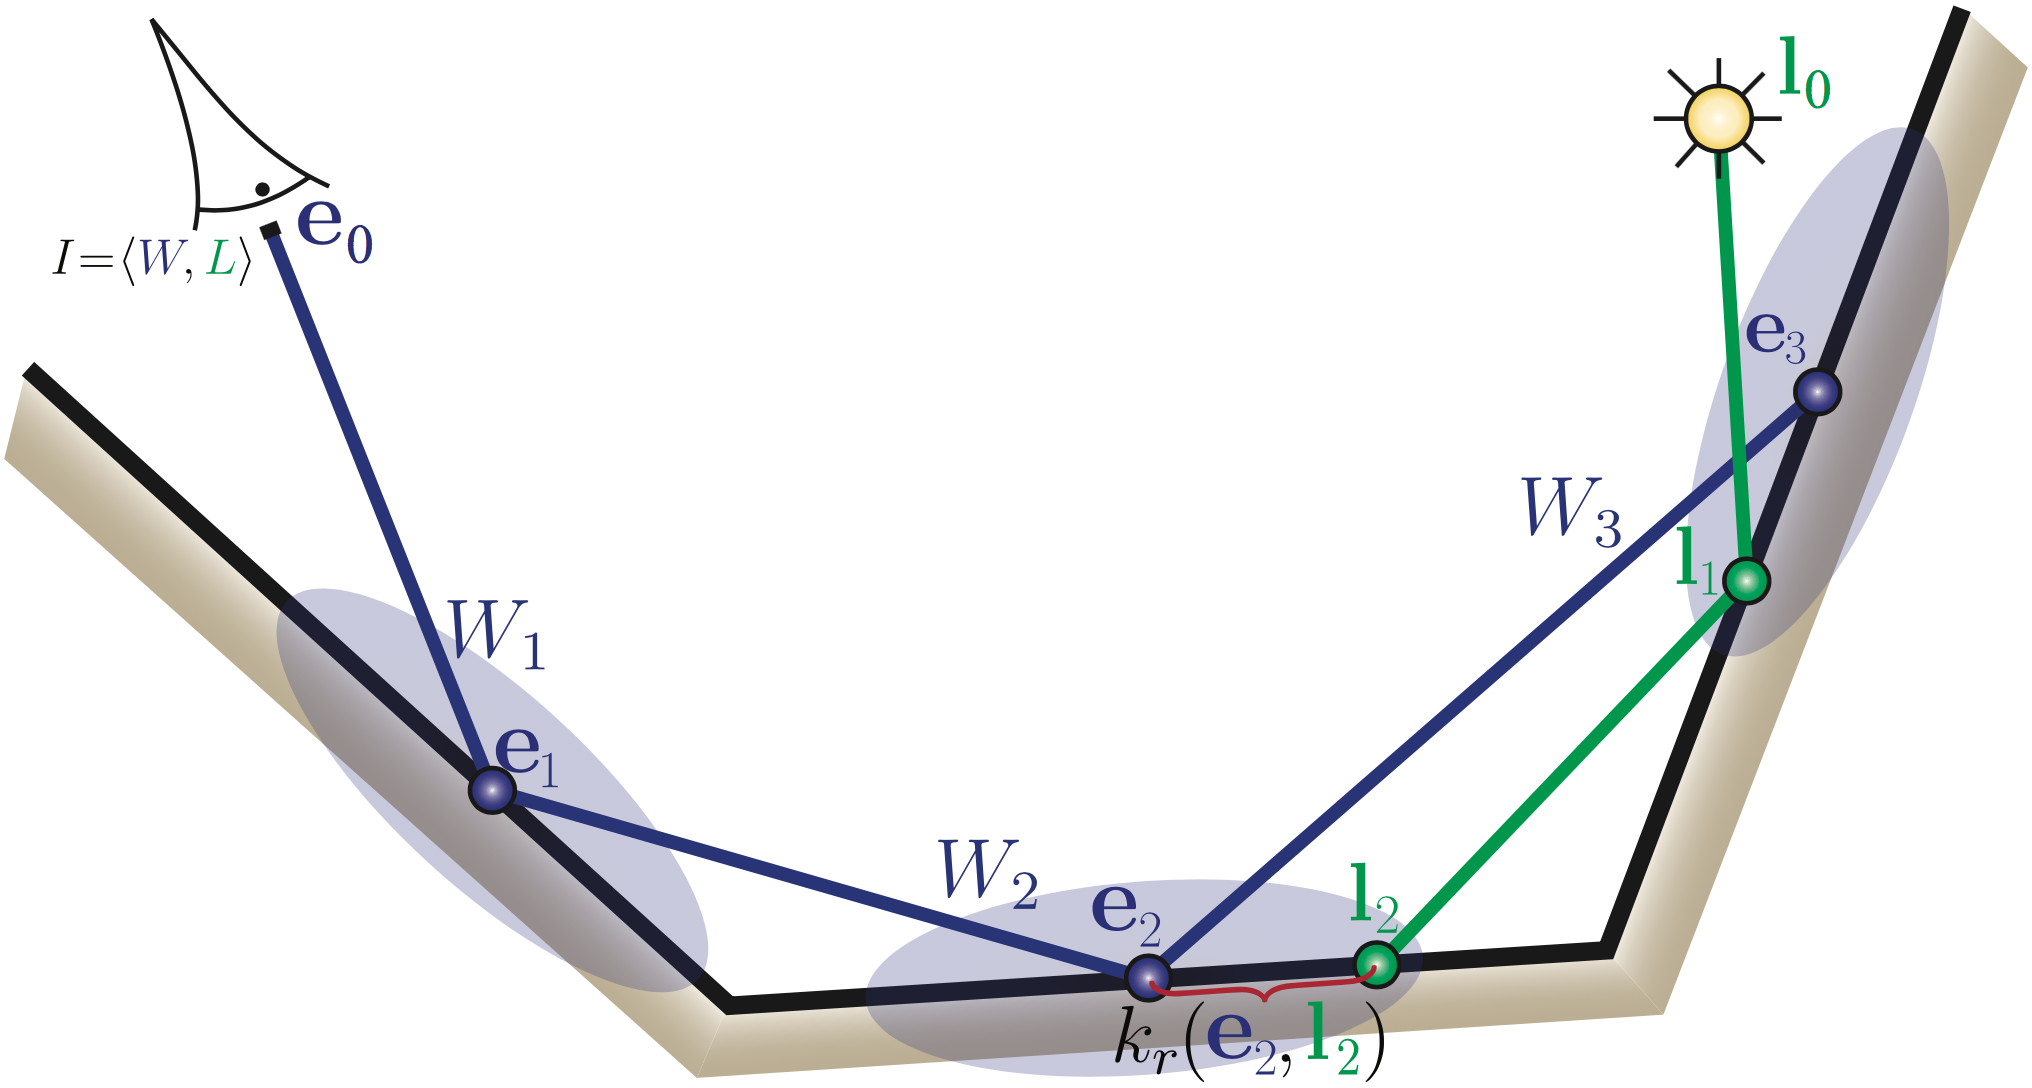
\includegraphics[width=0.65\textwidth]{figures/pm/path-space-estimation}
	\caption{路径空间的像素辐射亮度值估计,摄像机光线($eye-\mathbf{e}_1-\mathbf{e}_2$)与光源光线($light-\mathbf{l}_1-\mathbf{l}_2$)通过一个核函数$k_r$进行连接}
	\label{f:pm-path-space}
\end{figure}

这个新的表述形式使得我们可以将统计中核平滑相关的一些结论运用于PPM中最优带宽的选择。


\begin{figure}
	\sidecaption
	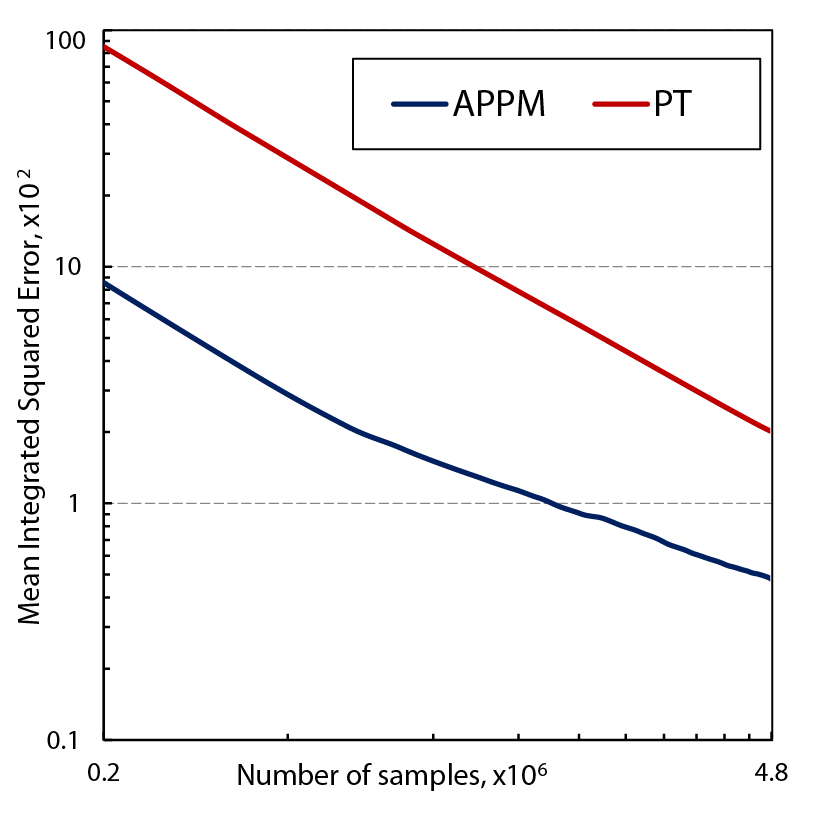
\includegraphics[width=0.65\textwidth]{figures/pm/pppm-error}
	\caption{路径空间的像素辐射亮度值估计,摄像机光线($eye-\mathbf{e}_1-\mathbf{e}_2$)与光源光线($light-\mathbf{l}_1-\mathbf{l}_2$)通过一个核函数$k_r$进行连接}
	\label{f:pm-pppm-error}
\end{figure}

这是PPM中辐射亮度估计的误差分析的结果,所以可以将误差分析放到这里作为基础。即误差分析的目的或结果就是用来指导适应性PPM,这有点和上一章的降噪技术类似。


\section{顶点连接与合并}\label{sec:pm-vcm}
尽管光子映射具有如处理SDS路径等的一些特性,它也有一些缺点:首先,它相较于传统的蒙特卡洛方法(其收敛速度为$O(N^{-1})$)具有更慢的收敛速度$O(N^{-2/3})$;其次,光子仅能被记录在漫反射表面上,因此很难处理具有较多光泽面或镜面的场景;最后,由于使用光子密度估计的近似方法,它需要非常多的光子数量才能达到比较精确的结果,因此其很难独立成为一种健壮的全局光照技术。

例如图\ref{f:pm-bpt-vs-ppm}所示,PPM能够很好地处理由镜子和花瓶形成的SDS焦散效果\footnote{这里其实是光从光源出发经过镜子镜面反射后落在花瓶表面上形成焦散面,然后摄像机发出的光线经过镜子镜面反射落在花瓶的焦散面上,形成SDS路径。},同样的效果在双向路径追踪(左一图)中则几乎无法处理;但是对于所有间接漫反射面\footnote{直接漫反射是通过直接光照计算的。}的光照计算,PPM的计算结果却呈现较大的误差,最右边小图显示了BPT和PPM在本节即将讨论的VCM中的相对贡献分布,可以看出窗户及墙面等大部分不能被光源直接照射的漫反射面的误差都很大。

\begin{figure}
\begin{fullwidth}	
	\includegraphics[width=1.\thewidth]{figures/pm/bpt-vs-ppm}
	\caption{分别使用BPT,PPM以及VCM计算30分钟后的结果对比,注意左上角的聚光灯投向镜子,然后经过镜面反射后照在花瓶及桌面上,右边的聚光灯也仅照射在桌面上,因此场景大部分环境都是间接光。这里可以看到BPT不能有效处理SDS焦散效果,而PPM在计算间接漫反射光照时误差比较大,VCM能够有效地联合BPT和PPM两种技术的优点,能够比较健壮地捕捉整个场景的光照。最右边的图显示了两种技术的相对光照贡献对比(图片来自\cite{a:LightTransportSimulationwithVertexConnectionandMerging})}
	\label{f:pm-bpt-vs-ppm}
\end{fullwidth}
\end{figure}

双向路径追踪和光子映射技术都具有各自的优点,因此我们很自然地希望能够将两者有效地组合起来,使能够综合它们各自的特点。传统的光子映射技术首先将渲染方程按照路径类型进行细分(例如本章第\ref{sec:pm-radiance-estimate-at-a-surface}节将光照划分为直接光照,光泽/镜面反射,焦散效果以及间接漫反射四种类型),然后对不同类型的路径使用不同的渲染技术,然而这是一种非此即彼的组合方法:即一种路径类型要么使用蒙特卡洛方法,要么使用光子映射技术,这并不是一种很好的组合方式,例如图\ref{f:pm-bpt-vs-ppm}最右边小图中绿色区域的部分,就是同时使用BPT和PPM进行计算的区域。

那么我们需要怎样更好的组合方式呢?答案是复合重要性采样,它能针对相同的路径(采样空间),将满足不同概率密度分布的样本组合起来,使能够兼顾每种采样技术的重要性。这即是要求针对相同的路径可以同时使用双向路径追踪和光子映射进行采样计算。

然而,复合重要性采样要求不同的概率密度分布函数具有相同的作用域,而我们已知双向路径追踪和光子映射具有完全不同的表述形式,甚至目前光子映射算法还没有一个“概率密度函数”。因此,有效组合光子映射和双向路径追踪技术的关键是将它们表述在一个统一的框架之下,\cite{a:LightTransportSimulationwithVertexConnectionandMerging}和\cite{a:APathSpaceExtensionforRobustLightTransportSimulation}同时独立地提出了这样的统一框架。

以下首先简要回顾一些本节需要用到的基础知识,如重要性采样以及双向追踪技术中的一些概念等,然后详细介绍顶点连接与合并相关的思路及算法。





\subsection{预备知识回顾}
对于积分$I={\rm \int}_{\Omega}f(x){\rm d}\mu (x)$,蒙特卡洛方法使用服从概率密度函数$p$分布的$n$个样本$X_1,\cdots,X_n$来近似:

\begin{equation}
	\hat{I}= \cfrac{1}{n}\sum^{n}_{i=1} \cfrac{f(X_i)}{p(X_i)}
\end{equation}

可以证明,上述估计是无偏,所以其误差仅由方差构成:

\begin{equation}
	V[F]=E[F^{2}]-E[F]^{2}={\rm \int}_{\Omega} \cfrac{f^{2}(x)}{p(x)}{\rm d}\mu (x)-I^{2}
\end{equation}

由上式可以看出,蒙特卡洛估计的方差严重依赖于采样分布$p$,理想情况下,如果$p$正比于被积函数$f$,那么其估计的方差为0。然后由于计算正比于$f$的概率密度函数需要知道被估量的真实值,即:$p=f/I$,而$I$正是我们需要估计的量,所以我们无法得到理想的概率密度函数$p$。然而通过使$p$的形状更近似于$f$的分布,仍然可以减小方差的值,我们称这样的技术为重要性采样(importance sampling)\mathindex{重要性采样}{importance sampling}。

通常我们并不知道被积函数的确切形式,我们可以使用多个分布函数进行采样,其中使用的每一个概率分布函数$p_i$称为一个采样技术(sampling technique)\mathindex{采样技术}{sampling technique},很显然,每一个采样技术将导致不同的方差以及其样本值对估计值不同的重要程度,因此我们的目标是组合不同的采样技术,使其结果对估计的贡献值最大,这种技术称为复合重要性采样(multiple importance sampling)\mathindex{复合重要性采样}{multiple importance sampling},其组合估计为:

\begin{equation}\label{e:pm-mis}
	\hat{I}=\sum^{m}_{i=1} \cfrac{1}{n_i}\sum^{n_i}_{j=1}w_i(X_{i,j}) \cfrac{f(X_{i,j})}{p_i(X_{i,j})}
\end{equation}

\noindent 这里$i$表示$m$不同的采样技术,$n_i$表示每种采样技术对应的样本数量,权重系数$w_i(X_{i,j})=[n_ip_i(x)]^{\beta}/\sum^{n}_{k=1}[n_kp_k(x)]^{\beta}$称为一个幂启发式(power heuristic)\myindex{幂启发式}{power heuristic},该权重系数用来使上述组合的估计的误差最小,当$\beta=1$时称为平衡启发式(更多相关知识详见第5章的内容),可以证明,当$\sum_iw_i(x)=1$(因此该式表述的是一种加权组合(weighted combination)\myindex{加权组合}{weighted combination})时,式\ref{e:pm-mis}表述的组合估计是无偏的。

式\ref{e:pm-mis}为我们提供了一种组合多种采样技术的简单而有效的方法,并且能够给予那些贡献值更大的样本以更大的权重。例如对于第4章中讨论的计算一个光泽面的来自圆形面积光源的光照贡献,当光源面积较小时,对光源面积分布函数进行采样将得到更优的结果,而当光源面积足够大时,直接对光泽面的BRDF分布函数进行方向采样得到的结果更优,而更好的办法就是使用上面讨论的复合重要性采样来组合两种采样技术。

有了上述的基础,使用复合重要性采样技术的步骤可以分为三步:首先,设计或选取一系列不同的重要性采样技术$p_1,\cdots,p_n$,例如这些采样技术可能能够比较好地近似$f$作用域上的某些部分,这样每种采样技术得到的样本值都可能比较大;其次,决定每个采样技术使用的样本数量$n_i$,这通常都是根据$f$和$p_i$的一些特征预先定义好的(例如在后面即将讨论的BPT和PPM的组合中,BPT对应的采样技术的样本数量通常是1,而PPM对于的采样技术的样本数量是其参与估计的光子数量);最后,使用式\ref{e:pm-mis}计算最终的加权组合估计值。




\paragraph{路径采样技术}
那么,在路径追踪技术中,一种采样技术是如何定义的呢,或者是复合重要性采样如何运用于路径追踪技术。

在传统的单向路径追踪(unidirectional path tracing)\myindex{单向路径追踪}{unidirectional path tracing}技术中,很显然它只包含一种采样技术:即首先从摄像机经过某个像素区域内的一个随机位置开始,然后光线在场景中的传播过程中通过对每个顶点处的BRDF分布采样来反射/折射光线,最后直到随机的BRDF方向采样击中某个光源或者被某种终止条件(如俄罗斯轮盘)丢弃。在这个过程中,对于所有路径样本,它们都使用同一个分布函数采样而得。如果算上从光源出发直到击中摄像机的反向路径采样,则单向路径追踪总共包含2中采样技术,如图\ref{f:pm-sampling-techniques}(a)所示。需要注意的是,单向路径的长短并不能形成不同的采样技术,因为其使用的概率分布函数的形式没变,只是在该分布下作用域内某些区域的取值很小或者为0。

\begin{myshaded}
	为什么单向路径追踪包含两种采样技术?这是因为前向路径的概率分布函数为像素区域中均匀分布与路径中各个BRDF及可见性函数的乘积,而反向路径的概率分布函数为光源分布函数与路径中各个BRDF及可见性函数的乘积,由此可见这两个是完全不同的概率分布函数,因此单向路径追踪对应2中采样技术。
\end{myshaded}

对于双向路径采样,它通过连接两条分别来自摄像机和光源的子路径形成一条完全路径,其中来自光源子路径的$s$个顶点和来自摄像机子路径的$t$个顶点连接形成一条包含$s+t$个顶点的长度为$k=s+1-1$的全路径。每条路径的概率密度函数为两条子路径概率密度函数的乘积,可表述为:

\begin{equation}\label{e:pm-mis-pdf}
	p_{s,t}(\vec{x}_{s,t})=\Biggl(p(y_1)\prod^{s-1}_{i=1}p(y_{i+1}|y_i)\Biggl)\Biggl(p(z_1)\prod^{t-1}_{i=1}p(z_{i+1}|z_i)\Biggl)
\end{equation}

\noindent 这里$\vec{x}_{s,t}$表示一条由$s$个光源子路径顶点和$t$个摄像机子路径顶点组成的全路径,$p(y_1)$表示光源的面积分布,而$p(z_1)$表示像素范围内随机位置的分布,$p(y|x)$表示由顶点$x$向顶点$y$方向的概率分布。

\begin{figure}
	\sidecaption
	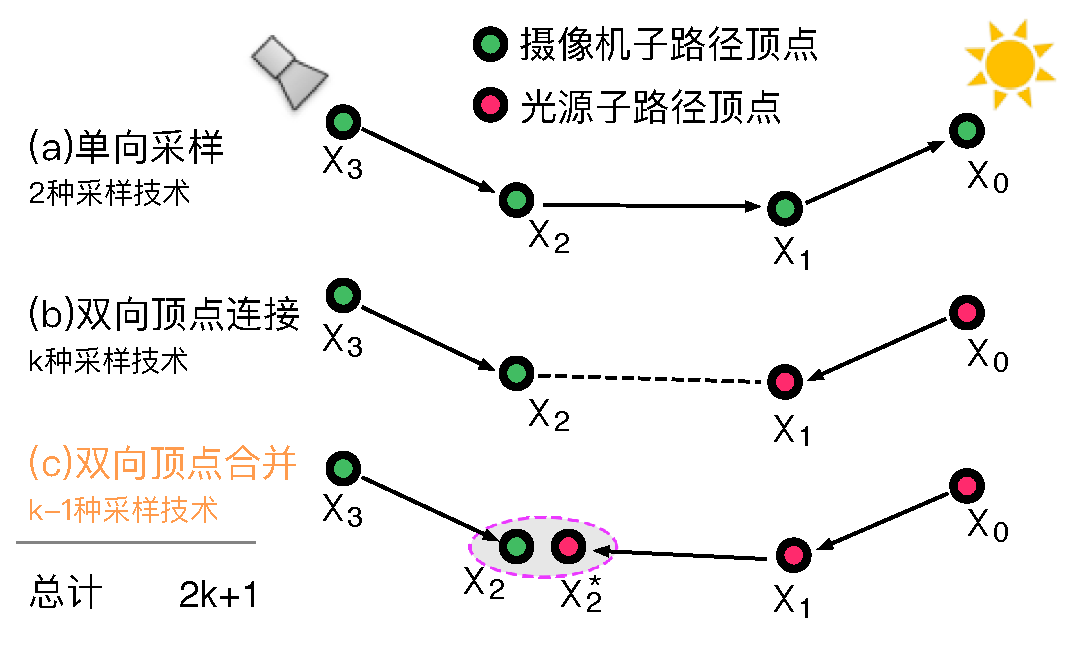
\includegraphics[width=.65\textwidth]{figures/pm/sampling-techniques}
	\caption{路径采样使用的不同的采样技术,对于路径长度为$k$(这里$k=3$)的全路径,传统的单向路径采样使用2中采样技术,双向路径采样增加$k$中采样技术,而顶点合并增加$k-1$种新的采样技术}
	\label{f:pm-sampling-techniques}
\end{figure}

很显然,在双向路径追踪技术中,对于相同长度$k$的全路径,不同的$s$和$t$形成的路径的概率密度函数是不同的\footnote{注意,对于式\ref{e:pm-mis-pdf},不能简单地看成为光源面积分布$p_(y_1)$,像素位置分布$p(z_1)$以及中间各路径顶点BRDF分布和可见性函数几项的乘积,这里两条路径的连接处并没有遵循对应的BRDF分布,而是直接连接形成一条全路径,这导致了每个$s,t$的组合具有完全不同的概率分布。},也因此对于整个路径空间,每个路径长度对应的路径的概率分布也是不同的,因此每一个长度$k$以及对应的每一个$s,t$的组合都构成一个不同的采样技术。长度为$k$的双向路径采样一共包含$k$中采样技术(这里排除了包含$s=0,t=k+1$以及$s=k+1,t=0$的两种特殊情况,即单向路径采样),如图\ref{f:pm-sampling-techniques}(b)所示。

由此,双向路径追踪下的复合重要性采样估计可以表述为:

\begin{equation}\label{e:pm-bpt-mis}
	\hat{I}=\sum^{\infty}_{M=1}\sum^{M+1}_{s=0}w_{s,t}(\vec{x}_{s,t}) \cfrac{f(\vec{x}_{s,t})}{p_{s,t}(\vec{x}_{s,t})}
\end{equation}

\noindent 为了表述简便这里定义$t=M+1-s$,通常这里设置$n_i=1$(参见\cite{a:OptimallyCombiningSamplingTechniquesforMonteCarloRendering})。

至此,我们便复习了理解顶点合并技术需要的全部基础知识,在下一节我们还将讨论顶点合并技术并且看到它为长度为$k$的全路径额外增加$k-1$种采样技术,如图\ref{f:pm-sampling-techniques}(c)所示。





\subsection{顶点合并}
传统的光子映射技术通过对光子图使用概率密度估计来近似某个漫反射点$x$处沿$\omega$方向的辐射亮度,其辐射亮度估计可表述为\cite{a:GlobalIlluminationusingPhotonMaps}:

\begin{equation}
	L_s(x,\omega)\approx\sum_{j}K_r(||x-x_j||)\rho_s(w_j,x,\omega)\Phi_j
\end{equation}

\noindent 这里$K_r$是以$r$为半径(带宽)的2D的过滤核函数,$j$参数遍历距离$r$范围内的光子,$x_{j}$和$\omega_j$分别表示每个光子的位置及其入射的方向,$\Phi_i$表示其辐射通量,$\rho_s(w_j,x,\omega)$表示顶点$x$处入射方向为$\omega_j$出射方向为$\omega$的BRDF值。

很显然,光子映射和双向路径追踪分别使用两种完全不同的数学公式,双向路径追踪是一个路径的积分形式,要想对两种技术按照复合重要性采样进行组合,我们还需要将光子映射也转换为路径的积分形式,以及计算每条路径的概率密度函数。

根据\cite{a:Densityestimationforstatisticsanddataanalysis},概率密度估计仍然可以表述为积分的形式,因此我们可以将使用光子密度估计的光照传输公式表述为:

\begin{equation}
	I^{'}_i={\rm \int}_{\Omega^{'}}f^{'}_j(\vec{x}){\rm d}\mu(\vec{x})=I_j+B_j
\end{equation}

\noindent 这里$f^{'}_j$表示包含了光子密度估计对贡献测量值函数的影响,$\Omega^{'}$称为扩展路径空间(extended path space)\myindex{扩展路径空间}{extended path space},$B_j$表示光子密度估计相关的偏差。

为了建立测量函数$f^{'}_j$所表示的路径,以及推导其对应的概率密度分布,我们使用一种称为顶点合并(vertex merging)\myindex{顶点合并}{vertex merging}的技术,直观上理解,顶点合并可以看成是将一个很小空间范围内的光子的顶点和待估计辐射通量位置处的顶点合并为一个顶点。如图\ref{f:pm-vcm}所示,待估计辐射通量的顶点为$x_s$,其附近参与估计的光子所在的顶点为$x^{*}_{s}$,在图\ref{f:pm-vcm}(b)中,这两个顶点被合并至$x_s$处,形成一条和传统双向路径追踪中两条子路径末端直接连接而成的全路径,我们称这种路径为常规路径(regular path)\myindex{常规路径}{regular path},而称合并前的原始路径为扩展路径(extended path)\myindex{扩展路径}{extended path}。从图\ref{f:pm-vcm}可以看出,常规路径为$\bar{x}=x_0\cdots x_{s-1},x_s\cdots x_k$,而其对应的扩展路径为$\bar{x}^{*}=x_0\cdots x^{*}_{s},x_s\cdots x_k$,常规路径的长度为$k$,而扩展路径的长度为$k+1$。

\begin{figure}
\sidecaption
	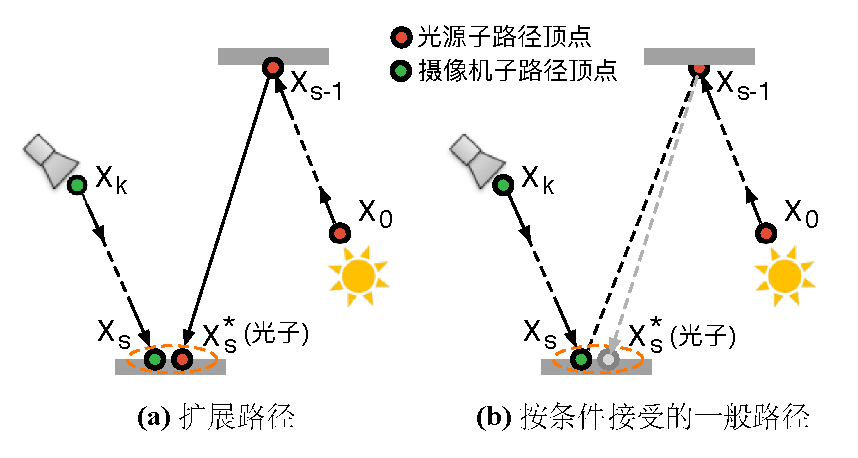
\includegraphics[width=.65\textwidth]{figures/pm/vcm}
	\caption{(a)光子映射可以被看做是对长度为$k+1$,包含$k+2$个顶点的扩展路径进行采样;(b)为了兼容BPT对应的路径积分框架,这里将上述过程解释为对该条扩展路径对应的常规路径进行采样,但是该条路径按照光子落于估计半径范围内的概率被接受}
	\label{f:pm-vcm}
\end{figure}

通过这样的方式生成的扩展路径的概率密度函数可以简单地表述为所有顶点概率密度函数的乘积(包括光子顶点$x^{*}_s$):

\begin{equation}\label{e:pm-extended-path-pdf}
\begin{aligned}
	p(\bar{x}^{*})&=p_{s+1,t}(\bar{x}_{s+1,t})\\
	&=\Biggl(p(y_1)\prod^{s}_{i=1}p(y_{i+1}|y_i)\Biggl)\Biggl(p(z_1)\prod^{t-1}_{i=1}p(z_{i+1}|z_i)\Biggl)
\end{aligned}
\end{equation}

我们已经将光子映射定义为一种在扩展路径空间下的采样技术,以及其对应的概率密度函数,因此我们可以直接使用上述定义对光子映射技术使用复合重要性采样:即和双向路径追踪的复合重要性采样类似,路径上每一个不同位置处被运用辐射亮度估计都被对应一种不同的采样技术,最后对所有这些采样技术的值进行加权组合,例如\cite{a:BidirectionalPhotonMapping}。

然而,我们并不能直接将像素值的估计在BPT和PM之间进行复合重要性组合,这是因为,对于给定长度的路径,相较于使用BPT采样得到的常规路径,使用PM采样得到的扩展路径拥有一个额外的顶点,即光子所在的位置$x^{*}_s$。因此,扩展路径空间对应的概率密度函数比常规路径空间的概率密度函数的作用域拥有跟高的维度,而复合重要性采样技术中的幂启发式依赖于所有概率密度函数具有相同的定义域以产生一个有意义的权重值。

所以,为了组合BPT和PM并对它们运用复合重要性采样,我们需要将具有相同路径长度并分别通过BPT和PM进行采样的概率密度函数表述在相同的测量空间,任意选取常规路径空间和扩展路径空间都是合适的,例如\cite{a:APathSpaceExtensionforRobustLightTransportSimulation}选择使用扩展空间,而\cite{a:LightTransportSimulationwithVertexConnectionandMerging}选择常规空间,它们两者本质上产生相同的结果,以下我们以后者为例进行介绍,因为这可以保持原始路径积分公式及其相关技术不需要发生改变,同时其过程更易于理解。





\subsubsection{光子映射在常规路径下的采样}
为了将光子映射视作在常规(而不是扩展)路径空间的采样,\cite{a:LightTransportSimulationwithVertexConnectionandMerging}使用顶点合并(vertex merging)\myindex{顶点合并}{vertex merging}的技术,将光子映射产生的全路径中光子所在的顶点$x^{*}_s$移除掉,形成一条常规路径:$\bar{x}=x_0\cdots x_k$,如图\ref{f:pm-vcm}(b)所示,对于$x_s$周围距离$r$范围内的所有光子,每一个光子都产生一条这样的常规路径。这样光子映射使用的采样概率密度函数就和双向路径追踪使用的概率密度函数具有相同的定义域\footnote{与之相对的是,我们也可以选择以扩展路径空间为基准,例如\cite{a:APathSpaceExtensionforRobustLightTransportSimulation},这时我们只需要将BPT和PM中具有相同数量顶点(包括参与光子密度估计的顶点$x^{*}_s$)路径的样本进行复合重要性组合即可。},因此它们之间可以进行复合重要性复合。由此也可以看出,对于长度为$k$的路径,光子映射能够增加$k-1$种新的采样技术,它们分别对应于路径内部各顶点处的合并操作,如图\ref{f:pm-sampling-techniques}(c)所示。

我们应该怎样解释这样一条光子映射产生的常规路径呢?首先该路径的贡献值显然是不变的,每个采样值按照传统的光子映射算法计算而出,我们需要解释的是其使用的概率密度函数的形式及其逻辑。

式\ref{e:pm-extended-path-pdf}表示的光子映射产生的扩展路径对应的概率密度函数,在常规路径空间下可以划分成两部分:$p_{VM}(\bar{x})=P_{acc}(\bar{x})p_{VC}(\bar{x})$,其中$p_{VC}(\bar{x})$表示按传统的BPT顶点连接技术产生的常规路径对应的概率密度分布(式\ref{e:pm-mis-pdf});而$P_{acc}(\bar{x})$表示这条路径被接受的概率。在BPT中,$x_{s-1}$直接和$x_s$相连(除非它们不可见),然而在PM中,$x_{s-1}$和$x_s$能否相连接取决于$x^{*}_s$是否落于$x_s$点附近距离为$r$的范围内,因此:

\begin{equation}
\begin{aligned}
	P_{acc}(\bar{x})&=Pr(||x_s-x^{*}_s||<r)={\rm \int}_{\mathcal{A}_{\mathcal{M}}}p(x|x_{s-1}){\rm d}x\\
	&\approx |\mathcal{A}_{\mathcal{M}}|p(x^{*}_s|x_{s-1})\approx\pi r^{2}p(x^{*}_s|x_{s-1})
\end{aligned}
\end{equation}

这里$\mathcal{A}_{\mathcal{M}}=\{x\in\mathcal{M}\mid||x_s-x||\leq r \}$表示$x_s$周围距离$r$内所有顶点的集合。要得到上式的解析解是非常困难的,这里可以借助于传统渐进式光子映射技术的一个假设:即$\mathcal{A}_{\mathcal{M}}$范围内的概率密度是常数,因此$p(x_{s-1}|x)$能够从积分中提取出来并使用$p(x^{*}_s|x_{s-1})$代替。需要注意的是,上述的假设在$x_{s-1}$为光泽面时其计算的精度会降低,但是随着带宽$r$逐渐收敛至0,该近似值则会逐渐收敛到真实值。





\subsubsection{统一的公式形式}
通过使用顶点合并,我们将光子映射表述为一种在常规路径空间下的采样技术,并得到了其概率密度函数,因此我们便可以将双向路径追踪和光子映射两种采样技术通过复合重要性采样组合起来,得到一个误差更小的估计。我们称这种组合的渲染算法为顶点连接与合并(vertex connection and merging,VCM)\myindex{顶点连接与合并}{vertex connection and merging}。与之对应,\cite{a:APathSpaceExtensionforRobustLightTransportSimulation}针对扩展路径空间对BPT和PM两种技术的复合重要性组合称为统一路径采样(unified path sampling,UPS)\myindex{统一路径采样}{unified path sampling},由于这两种技术本质上是一致的,所以也统称这种技术为VCM/UPS。

使用$\hat{I}_{VC}$表示通过顶点连接(BPT)产生的估计值,$\hat{I}_{VM}$表示通过顶点合并产生的估计值:

\begin{equation}\label{e:pm-bpt-and-pm-mis}
\begin{aligned}	
	\hat{I}=&C_{VC}+C_{VM}\\
		   =& \cfrac{1}{n_{VC}}\sum^{n_{VC}}_{l=1}\sum_{s\geq 0,t\geq 0}w_{VC,s,t}\hat{I}_{VC}(\bar{x}_l)+\\
		   & \cfrac{1}{n_{VM}}\sum^{n_{VM}}_{l=1}\sum_{s\geq 2,t\geq 2}w_{VM,s,t}\hat{I}_{VM}(\bar{x}_l)
\end{aligned}
\end{equation}

\noindent 上式可以看成是对双向路径追踪\cite{a:RobustMonteCarloMethodsforLightTransportSimulation}(即式\ref{e:pm-bpt-mis})的一个扩展,针对摄像机子路径上的每个顶点,它们分别被$n_{VC}$条光源子路径上的顶点相连接,或者与$n_{VM}$个光源子路径的顶点发生合并。注意这里BPT采样部分包含了2种单向路径采样技术($t=0$或者$s=0$),而PM采样部分则排除了每个子路径首尾两个顶点($t=0,1$或者$s=0,1$)的合并:光源直接可见的点使用直接光计算贡献值更大,而对于摄像机可见的顶点,光子密度估计的误差很大。

通过式\ref{e:pm-bpt-and-pm-mis}还可以实现在UPT,BPT和PM之间的自由切换和组合,例如设置$n_{VC}=0$,则该算法变为纯光子映射;如果设置$n_{VM}=0$,则该算法变为双向路径追踪,如果同时设置$n_{VM}=0$,并且限制$s=0$或者$t=0$,则该算法变为单向路径追踪。实际上Renderman\footnote{参见:\url{https://rmanwiki.pixar.com/display/REN/PxrVCM}。}就通过connectPaths和mergePaths两个参数来控制是否需要双向路径采样或光子映射采样,从而实现三者之间的无缝切换,这可以用来对比不同的技术对光照的不同贡献。

式\ref{e:pm-bpt-and-pm-mis}中的权重系数通过使用幂启发式计算可得:

\begin{equation}\label{e:pm-vcm-weight}
	w_{v,s,t}(\bar{x})= \cfrac{n^{\beta}_vp^{\beta}_{v,s,t}(\bar{x})}{n^{\beta}_{VC}\sum_{s^{'}\geq 0,t^{'}\geq 0}p^{\beta}_{VC,s^{'},t^{'}}(\bar{x})+n^{\beta}_{VM}\sum_{s^{'}\geq 2,t^{'}\geq 2}p^{\beta}_{VM,s^{'},t^{'}}(\bar{x})}
\end{equation}

\noindent 这里$v$表示使用顶点连接($VC$)或者顶点合并($VM$)采样技术。由于幂启发式这样的观察计算的:即更大值的概率密度函数导致更低的方差,所以上式可以用来比较不同采样技术的相对贡献,如图\ref{f:pm-bpt-vs-ppm}最右边小图所示。

\begin{figure}
\begin{fullwidth}
	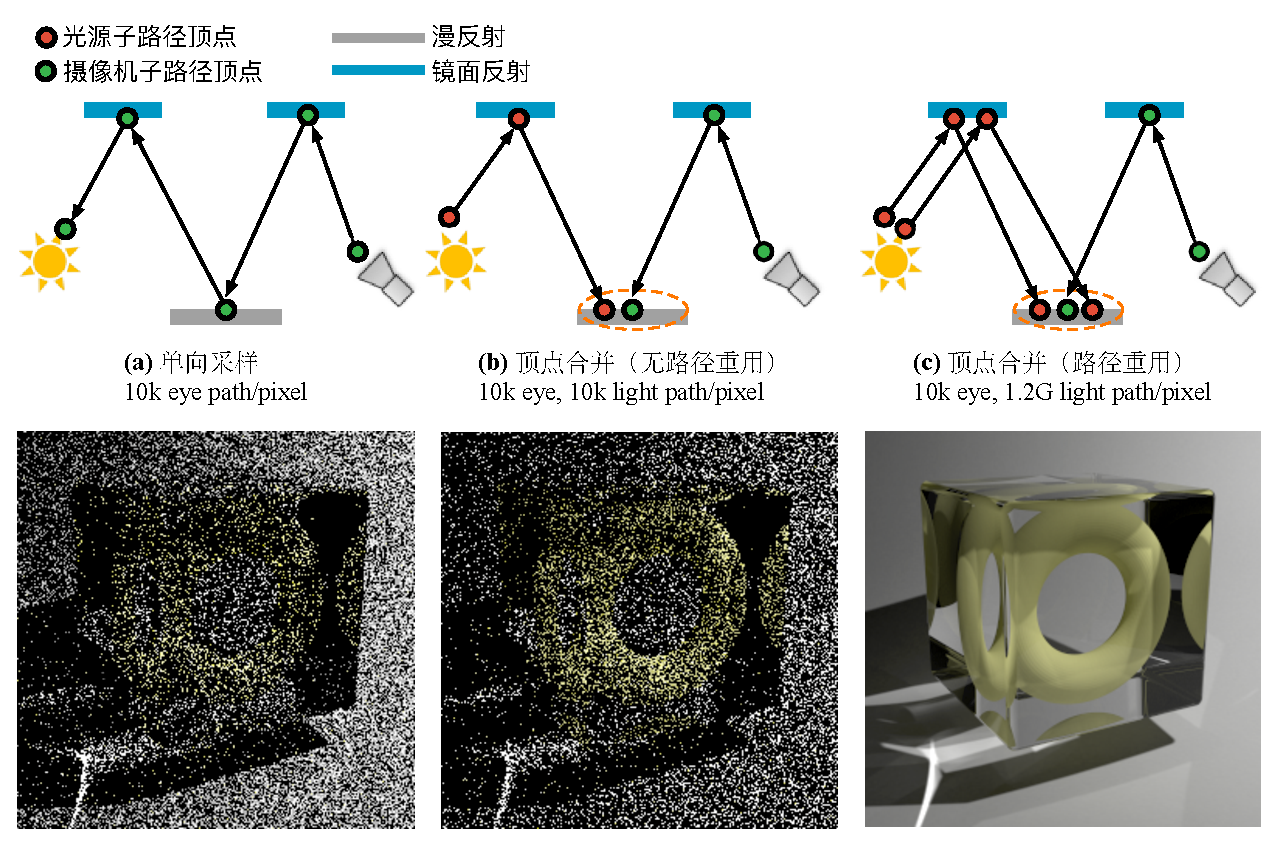
\includegraphics[width=\thewidth]{figures/pm/path-reuse}
	\caption{VCM能够解释为什么光子映射能够更健壮地处理SDS路径,这不是因为它能够更容易地找到这些路径,而是它能够更有效地重用光源子路径;如果没有高效的路径重用,PM的执行效率几乎和UPT一样低,因为BPT中最后顶点落在光源上的概率和PM中通过$x_{s-1}$发出的光照落于$\pi r^{2}$区域的概率都很低(图片来自\cite{a:LightTransportSimulationwithVertexConnectionandMerging})}
	\label{f:pm-path-reuse}
\end{fullwidth}
\end{figure}

此外,通过式\ref{e:pm-vcm-weight}还可以看出,每种采样技术使用的样本数量$n_v$对权重计算的影响很大。假设$n_{VC}=n_{VM}=1$,如果顶点$x_{s-1}$处于漫反射面,则$P_{acc}$值会非常小,因为从$x_{s-1}$对半空间随机采样落于一个很小的面积$\pi r^{2}$的几率很小,这就导致针对同一长度的单条路径,PM路径的贡献率要比BPT路径小得多。然而PM的特点是计算效率更高,它产生一条新的路径的成本就是一次最近邻查询的成本,相对BPT需要对完整的路径采样要高效的多。所以针对同一长度的路径,我们可以通过提高PM采样的数量$n_{VM}$来提高其贡献率,这样在那些其他采样技术的效率不如PM的地方,例如SDS路径,PM采样可以得到更低的误差,如图\ref{f:pm-path-reuse}所示。

因此$n_{VM}$的数量通常远远大于$n_{VC}$,实践中常设$n_{VC}=1$,而$n_{VM}$等于总的光源子路径的数量。这里设置$n_{VC}=1$的原因是因为渲染算法通常是迭代进行的,每个迭代通常只对每个像素发射一条摄像机路径,见下面算法的详细讨论。

算法\ref{a:pm-vcm}描述了VCM的一般实现。由于路径采样的计算量比较复杂,所以一般实现都是迭代进行的,这里每个迭代处理pixelCount个摄像机子路径和pixelCount个光源子路径(pixelCount为屏幕上总的像素数量),这解释了为什么$n_{VC}=1$。其次,由于BPT和PM均需要对路径进行重用,所以这里采样和PM一样的思路,将路径采样和贡献值计算分开成两个阶段。

\begin{algorithm}
\begin{lstlisting}[language=C++, mathescape]
void RENDER(r) {
	//阶段1:光源子路径采样
	lightPaths = TRACELIGHTPATHS(pixelCount) 
	CONNECTTOEYE(lightVertices) 
	BUILDRANGESEARCHSTRUCT(lightVertices)
	
	//阶段2:摄像机子路径采样,并且计算每条路径的像素值贡献
	for ( i = 1 to pixelCount ) {
		eyeVertex = TRACERAY(SAMPLEPIXEL(i)) 
		while ( eyeVertex is valid ) {
			//Unidirectional sampling (US) 
			if ( eyeVertex is emissive )
				ACCUM(eyeVertex, US, r, i) 
			
			//Vertex connection (VC)
			for ( lightVertex in lightPaths[i]||[SAMPLELIGHTPOINT()) 
				ACCUM(CONNECT(eyeVertex, lightVertex), VC, r, i) 
		
			//Vertex merging (VM)
			for ( lightVertex in RANGESEARCH(eyeVertex, r) )
				ACCUM(MERGE(eyeVertex, lightVertex), VM, r, i) 
			eyeVertex = CONTINUERANDOMWALK(eyeVertex) 
		}
	}
}
		
//累积每条路径的像素值贡献
void ACCUM(path, technique, r, i) {
	contrib = MEASUREMENTCONTRIBUTION(path, technique, r) 
	pdf = PDF(path, technique, r)
	weight = POWERHEURISTIC(path, technique, pdf )
	image[i] += weight * contrib / pdf
}
\end{lstlisting}
\caption{使用顶点连接与合并(VCM)渲染图形的伪代码,输入参数为一个最大顶点合并的距离$r$(算法来自\cite{a:LightTransportSimulationwithVertexConnectionandMerging})}
\label{a:pm-vcm}
\end{algorithm}

在第一个阶段,首先生成pixelCount条光源子路径,并构建光子图,这里其实将BPT和PM的光源子路径合并了,唯一不同的就是在漫反射表面处存储一个光子即可;在第二个阶段,首先对每个像素随机产生一条摄像机子路径,并使该路径在场景中随机行走直至满足终止条件,然后摄像机子路径的每个顶点与所有光源子路径进行连接或合并以计算各自对应的光照贡献,最后再按照权重系数累积计算最终的像素值。读者也可以进一步阅读该篇论文提供的开源代码\footnote{请参见:\url{https://github.com/SmallVCM/SmallVCM}}。

由于顶点合并引入了偏差,因此式\ref{e:pm-bpt-and-pm-mis}是有偏的,但是和PPM一样,通过渐进地减小合并半径$r$,方差和偏差在极限的情况下收敛至0,从而使估计变得一致。式\ref{e:pm-bpt-and-pm-mis}的渐进式变种可以表述为:

\begin{equation}
	\hat{I}_{VCM}= \cfrac{1}{N}\sum^{N}_{i=1}(C_{VC,i}+C_{VM,i})
\end{equation}

这里的$C_{VC,i}$和$C_{VM,i}$同式\ref{e:pm-bpt-and-pm-mis}中的相同,但是在每个迭代中使用一组不同的光源和摄像机子路径,以及一个逐步缩减的合并半径$r_i=r_1\sqrt{i^{\alpha-1}}$,这里$\alpha\in (0;1)$和渐进式光子映射中的参数一样。





\section{参与介质}\label{sec:pm-participating-media}
到目前为止,本章讨论的光子映射涉及的所有光照交互都发生于物体表面,这意味着辐射亮度$L$在表面与表面之间的传输过程中保持为常数,这在物体所处介质为真空的假设条件下是成立的,因为光子在真空中可以进行无障碍传输。然而,现实世界往往充满着各种介质(medium),例如空气,水,烟雾,云等等,光子在这些介质中并不能保持常数传播,这些介质会在光线的传播过程中会参与(participating)光线的交互,因此也称为参与介质(participating media)\myindex{参与介质}{participating media}。不同于前面讨论的表面的渲染,因为介质中每个点(介质中的粒子)都会参与光照交互,所以参与介质的渲染也称为体积渲染(volumetric rendering)\myindex{体积渲染}{volumetric rendering},不难看出,体积渲染的计算量要大得多。

我们在上一章已经讨论过怎样使用蒙特卡洛方法来模拟参与介质引起的各种效果,本节将扩展本章前面介绍的表面光子映射技术,使之能够处理参与介质。我们将看到,由于光子映射技术能够重用光线路径,大大加速了参与介质中需要的对周围全空间范围内的积分来计算每个点入射辐射照度的计算,更重要的是,由于光线在介质传播中的特性,我们推导出了一种区别于传统点采样(point sampling)\myindex{点采样}{point sampling}的新的光线采样形式:即光束采样(beam sampling)\myindex{光束采样}{beam sampling},这种新的采样技术不仅能够大大减少所需分配的光子数量,并且能够大大提升计算效率和渲染品质,使其成为当前乃至未来重要的参与介质渲染技术。




\subsection{光线在介质中的传播}
在计算机图形学中,参与介质通常被描述为一组具有散射性的微观粒子的集合,如图\ref{f:pm-participating-media}所示,由于这些粒子的尺寸非常小并且其位置随机分布,所以通常我们并不对单个粒子的光照传输特性进行表述,而是考虑整个粒子集合的概率行为;并且,这些粒子之间的空间分布被假设为远大于单个粒子本身的尺寸,这意味着随着光子在介质中传播并与粒子发生交互事件,该事件与光子接下来与其他粒子之间的交互事件是统计独立的(statistically independent)\myindex{统计独立的}{statistically independent}。

\begin{figure}
	\sidecaption
	\includegraphics[width=0.65\textwidth]{figures/pm/participating-media}
	\caption{参与介质被认为是一些微观散射粒子的组合,其物体几何形状为这些粒子所在体积的边界,当光线穿过这些介质时,其辐射亮度$L$会随着传输的距离而发生变化}
	\label{f:pm-participating-media}
\end{figure}




\subsubsection{消光系数:吸收和向外散射}
当光子穿过一组微观粒子构成的介质时,它可能完全不与任何粒子发生碰撞而继续不受影响的传播(就像在真空中一样),也可能与其中的一些粒子发生交互,从而影响光照的传输。光子与粒子发生交互的概率取决于该介质的消光系数(extinction coefficient)\myindex{消光系数}{extinction coefficient}$\sigma_t$,也称为衰减系数(attenuation coefficient)\myindex{衰减系数}{attenuation coefficient},其单位为$1/m$,它表示每单位距离对光的吸收率。

消光系数的值取决于介质中粒子的密度以及尺寸等物理特性,它是两种类型的光照交互作用的结果:即当光子与粒子发生交互时,它要么被粒子吸收(其光子能量被转化为另一种形式,例如热能),或者光子被散射到另一个方向;这两种交互事件发生的相对概率分别表述为吸收系数(absorption coefficient)$\sigma_a$,如图\ref{f:pm-medium-properties}(a)所示,和散射系数(scattering coefficient)$\sigma_s$,如图\ref{f:pm-medium-properties}(c)所示,因此消光系数可表述为:$\sigma_t=\sigma_a+\sigma_s$。需要注意的是,同$\sigma_t$一样,$\sigma_a$和$\sigma_s$的单位仍为$1/m$,因为在实际问题中我们更专注光束在其传输的一定厚度(thickness)内的衰减情况,而不是与单个粒子的交互行为。

由上述定义可知,吸收和散射描述的均是光子在单位长度距离传播过程中的衰减行为,当考虑一束光$L(\mathbf{x}\to\vec{\omega})$沿$\omega$方向穿过一个介质时(如图\ref{f:pm-participating-media}所示),由于该光束中光子的数量正比于该光束的辐射亮度$L(\mathbf{x}\to\vec{\omega})$,因此上述光束在介质中传播的净损失(net loss)可用微分方程表述为:

\begin{equation}\label{e:pm-net-loss}
\begin{aligned}
	(\vec{\omega}\cdot\nabla_t)L(\mathbf{x}\to\vec{\omega})=&-(\sigma_a(\mathbf{x})+\sigma_s(\mathbf{x}))L(\mathbf{x}\to\vec{\omega})\\
	=&-\sigma_t(\mathbf{x})L(\mathbf{x}\to\vec{\omega})
\end{aligned}
\end{equation}

\noindent 这里$(\vec{\omega}\cdot\nabla)$计算沿$\vec{\omega}$方向的方向导数,负数符号表示辐射亮度的减少。为了更直观地描述光束在介质中的传播,我们使用一个光束透射比(beam transmittance)\myindex{光束透射比}{beam transmittance}的概念来解上述的微分方程,记为$T_r$,光束透射比描述的是光束在介质中的两点之间沿光线传播后,保留下来的光子数量的分量,其他的光子则要么被吸收了,要么被散射到其他方向了。根据比尔定律(Beer’s Law)\mathindex{比尔定律}{Beer’s Law},即通过对式\ref{e:pm-net-loss}执行积分计算可得:

\begin{equation}\label{e:pm-transmittance}
	T_r(\mathbf{x}\leftrightarrow\mathbf{x}^{'})=e^{-\tau(\mathbf{x}\leftrightarrow\mathbf{x}^{'})}
\end{equation}

\noindent 其中,$\tau$称为光学厚度(optical thickness)\myindex{光学厚度}{optical thickness}或者光学深度(optical depth)\myindex{光学深度}{optical depth},它可以通过对消光系数沿一个线段执行积分计算而得:

\begin{equation}
	\tau(\mathbf{x}\leftrightarrow\mathbf{x}^{'})={\rm \int}^{d}_{0}\sigma_t(\mathbf{x}+t\vec{\omega}){\rm d}t
\end{equation}

\noindent 这里$\mathbf{x}+t\vec{\omega}$表示的是$\mathbf{x}$和$\mathbf{x}^{'}$之间的一条线段,其中$d=||\mathbf{x}^{'}-\mathbf{x}||$。在均质介质(homogeneous medium)\myindex{均质介质}{homogeneous medium}中,$\sigma_t$,$\sigma_s$和$\sigma_a$均是与位置无关的常数,则$\tau$可以简化为:

\begin{equation}
	\tau(\mathbf{x}\leftrightarrow\mathbf{x}^{'})=d\sigma_t
\end{equation}

光束透射比的值总是介于0和之间,当仅考虑吸收和向外散射时,透射比可以用于计算减少的辐射亮度(reduced radiance)\myindex{减少的辐射亮度}{reduced radiance}:

\begin{equation}
	L(\mathbf{x}\leftarrow\vec{\omega})=T_r(\mathbf{x}^{'}\leftrightarrow\mathbf{x})L(\mathbf{x}^{'}\to-\vec{\omega})
\end{equation}

\noindent 上式描述了辐射亮度在介质中的传播中怎样被减少了。不难看出,透射比在一条直线的三个点之间满足可乘性:

\begin{equation}
	T_r(\mathbf{x}\leftrightarrow\mathbf{x}^{''})=T_r(\mathbf{x}^{'}\leftrightarrow\mathbf{x}^{'})T_r(\mathbf{x}^{'}\leftrightarrow\mathbf{x}^{''})
\end{equation}

\noindent 其中,$\mathbf{x}^{'}$位于$\mathbf{x}$和$\mathbf{x}^{''}$之间。

我们将在第\ref{sec:pm-transmittance-estimate}详细介绍透射比的各种估计方法。




\subsubsection{向内散射和辐射}
光束在介质中的传播过程中,除了有原有入射辐射亮度的损失(即吸收和散射,如图\ref{f:pm-medium-properties}(a)和(c)所示),其辐射亮度也可能随着光束的传播而增加,这些增加的辐射亮度来源于向内散射和自发光。

粒子的散射行为在将$\vec{\omega}$方向的光子散射到其他方向的同时,也会将来自其他方向的入射光子散射到$\vec{\omega}$方向上,使增加原有光束的光子数量。我们称前者为向外散射(out-scattering)\myindex{向外散射}{out-scattering},如图\ref{f:pm-medium-properties}(c)所示,而称后者为向内散射(in-scattering)\myindex{向内散射}{in-scattering},如图\ref{f:pm-medium-properties}(d)所示。光子散射的方向分布使用后面即将介绍的相位函数描述,它跟表面的双向反射函数BRDF是类似的概念。

\begin{figure}
	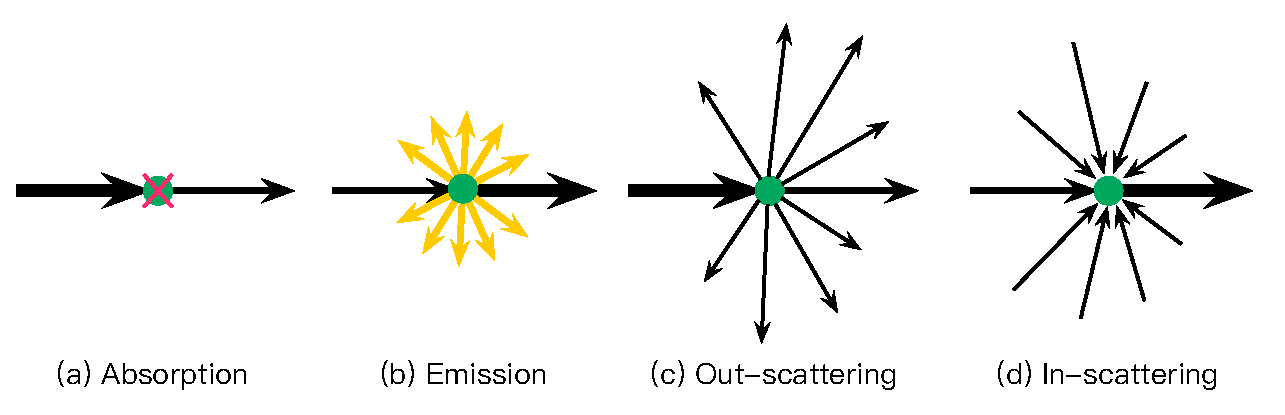
\includegraphics[width=1.\textwidth]{figures/pm/medium-properties}
	\caption{当光在介质中传播时,其最终的辐射亮度会根据以下四种交互发生变化:(a) 吸收,(b) 辐射,(c)向外散射以及(d)向内散射}
	\label{f:pm-medium-properties}
\end{figure}

假设向内散射在$\vec{\omega}$方向的辐射亮度为$L_i(\mathbf{x}\to\vec{\omega})$(将在下面讨论),同前面的吸收和向外散射,向内散射导致的辐射亮度的变化(这里是增加)可有微分方程表述为:

\begin{equation}\label{e:pm-in-scattering}
	(\vec{\omega}\cdot\nabla_i)L(\mathbf{x}\to\vec{\omega})=
	\sigma_s(\mathbf{x})L_i(\mathbf{x}\to\vec{\omega})
\end{equation}

同理,对于自发光的介质\footnote{注意,辐射传输理论中的自发光往往是指满足热平衡条件下不同形式能量的转换,例如这里使用吸收系数$\sigma_a$就表示这些发射的能量来自于吸收的能量部分,图形学中一般不模拟这种形式的自发光,而是直接使用光源,以下我们将忽略这种形式的光照的改变。},由于自发光导致的辐射亮度的增加也可以表述为:

\begin{equation}\label{e:pm-emission}
	(\vec{\omega}\cdot\nabla_e)L(\mathbf{x}\to\vec{\omega})=
	\sigma_a(\mathbf{x})L_e(\mathbf{x}\to\vec{\omega})
\end{equation}




\paragraph{相位函数}
在式\ref{e:pm-in-scattering}中,$L_i(\mathbf{x}\to\vec{\omega})$表示点$\mathbf{x}$处来自所有方向的光照最终散射到$\vec{\omega}$方向上的辐射亮度的总和,如图\ref{f:pm-medium-properties}(d)所示,它涉及对整个球面方向进行积分:

\begin{equation}
	L_i(\mathbf{x}\to\vec{\omega})={\rm \int}_{\Omega_{4\pi}}p(\mathbf{x},\vec{\omega}^{'}\to\vec{\omega})L(\mathbf{x}\leftarrow\vec{\omega}^{'}){\rm d}\vec{\omega}^{'}
\end{equation}

\noindent 这里$p(\mathbf{x},\vec{\omega}^{'}\to\vec{\omega})$称为一个相位函数(phase function)\myindex{相位函数}{phase function},其单位为$1/sr$,它描述光子在介质中某个位置处散射的方向分布,如图\ref{f:pm-phase-function}所示;相位函数的概念和表面的双向反射分布函数BRDF是类似的,其区别为相位函数用于介质内部,因此适用于整个球面空间的所有方向。此外,BRDF函数返回的是一个完整的散射函数的光照值,而相位函数仅仅返回一个相位的值,它必须乘以散射系数$\sigma_s$才能表示散射的光照结果,这也是式\ref{e:pm-in-scattering}中需要乘以散射系数的原因。所以,这里我们重新定义散射函数(scattering function)\myindex{散射函数}{scattering function}为:

\begin{equation}\label{e:pm-scattering}
\rho(\mathbf{x},\vec{\omega}^{'}\leftrightarrow\vec{\omega})=\begin{cases}
	\rho_s(\mathbf{x},\vec{\omega}^{'}\leftrightarrow\vec{\omega})&\text{$\mathbf{x}$在表面上}\\
	p(\mathbf{x},\vec{\omega}^{'}\leftrightarrow\vec{\omega})\sigma_s(\mathbf{x})&\text{$\mathbf{x}$在介质中}\\
\end{cases}
\end{equation}

同BRDF一样,相位函数也具有互换性(reciprocity),即$p(\mathbf{x},\vec{\omega}^{'}\to\vec{\omega})=p(\mathbf{x},\vec{\omega}^{'}\leftarrow\vec{\omega})$,因此以下我们统一使用标记:$p(\mathbf{x},\vec{\omega}^{'}\leftrightarrow\vec{\omega})$;并且它一般是归一化的,即对所有方向满足:

\begin{equation}
	{\rm \int}_{\Omega_{4\pi}}p(\mathbf{x},\vec{\omega}^{'}\leftrightarrow\vec{\omega}){\rm d}\vec{\omega}^{'}=1
\end{equation}

相位函数可以是各向同性的,它将光照均匀地散射到各个方向,对所有方向的值为一个常数$ \cfrac{1}{4\pi}$,例如图\ref{f:pm-phase-function}(b)所示;根据材质不同,相位函数更多呈现各向异性,例如其中一个被广泛使用的各向异性相位函数是Henyey-Greenstein相位函数\cite{a:Diffuseradiationinthegalaxy,a:EfficientMonteCarloMethodsforLightTransportinScatteringMedia}\myindex{Henyey-Greenstein相位函数}{Henyey-Greenstein phase function},其已被用于模拟云,海洋,皮肤等散射材质。

Henyey-Greenstein相位函数仅与散射的角度$\theta$有关:

\begin{equation}
	p_{HG}(\mathbf{x},\theta)= \cfrac{1-g^{2}}{4\pi(1+g^{2}-2g\cos{\theta})^{1.5}}
\end{equation}

\noindent 这里唯一的参数$g\in[-1,1]$用于决定散射的相对朝向:当$g<0$时相位呈后向分布,如图\ref{f:pm-phase-function}(a)所示,当$g>0$时相位呈前向分布,如图\ref{f:pm-phase-function}(c)所示,当$g=0$时则变为各向同性分布,如图\ref{f:pm-phase-function}(b)所示。读者可阅读\cite{a:EfficientMonteCarloMethodsforLightTransportinScatteringMedia}了解更多相位函数的例子。

\begin{figure}
\begin{fullwidth}
	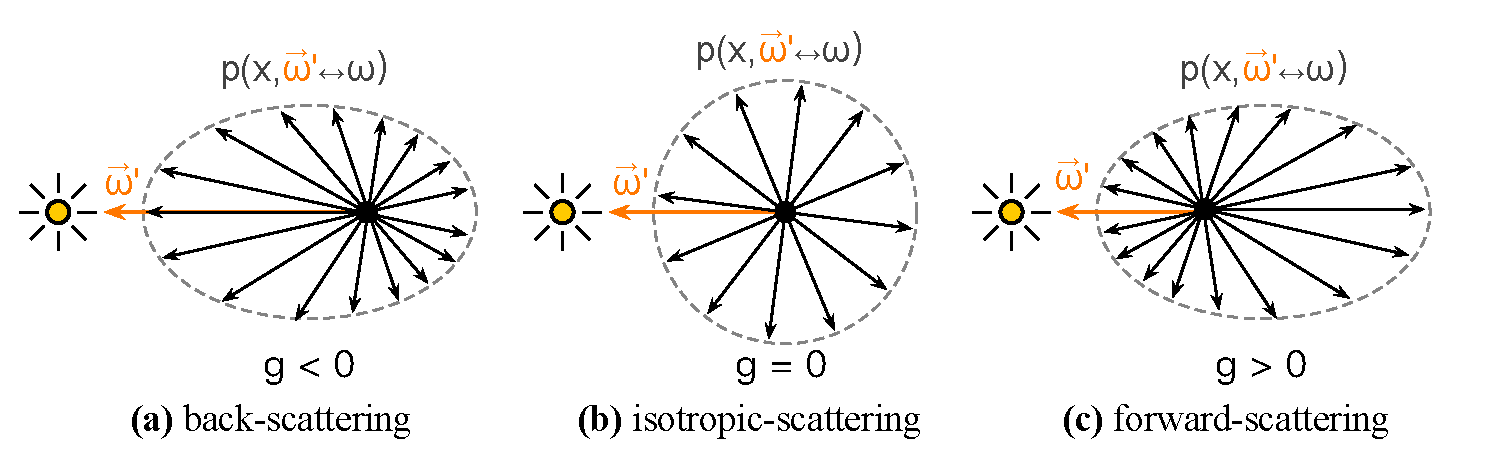
\includegraphics[width=\thewidth]{figures/pm/phase-function}
	\caption{相位函数描述的是介质内部任意位置$\mathbf{x}$处光子散射的方向分布,在最简单的情况下,光子被均匀地散射到各个方向(b),但是自然界中的很多材质具有更趋向于后向(a)或者前向(c)散射的方向分布}
	\label{f:pm-phase-function}
\end{fullwidth}
\end{figure}






\subsubsection{辐射传输方程}
我们已经讨论了光子在介质中的传输过程中可能发生的4种交互事件:即吸收,向外散射,自发光及向内散射(如图\ref{f:pm-medium-properties}所示),其中前两者会减小入射辐射亮度,而后两者会增加额外的辐射亮度,由此我们可以推导出一个完整的光照在介质中的传输模型,通过组合式\ref{e:pm-net-loss}和式\ref{e:pm-in-scattering},在介质中沿一条光束传输的光线其位于$\mathbf{x}$处辐射亮度的改变可以表述为(这里我们忽略了自发光):

\begin{equation}
	(\vec{\omega}\cdot\nabla_t)L(\mathbf{x}\to\vec{\omega})=-\sigma_t(\mathbf{x})L(\mathbf{x}\to\vec{\omega})+\sigma_s(\mathbf{x})L_i(\mathbf{x}\to\vec{\omega})
\end{equation}

\noindent 该方程称为辐射传输方程(radiative transport equation,RTE)\cite{a:RadiativeTransfer}\myindex{辐射传输方程}{radiative transport equation},它描述了光照在介质中传播的可能发生的交互事件。上式表述的是光线传输过程中位置$\mathbf{x}$处的光照改变,通过对介质内的整个传输长度进行积分,可以得到一个积分形式的辐射传输方程(如图\ref{f:pm-transmittance}所示):

\begin{equation}\label{e:pm-rte}
\begin{aligned}
	L(\mathbf{x}\leftarrow\vec{\omega})=&T_r(\mathbf{x}\leftrightarrow\mathbf{x}_s)L(\mathbf{x}_s\to -\vec{\omega})\\ &+{\rm \int}^{s}_{0}T_r(\mathbf{x}\leftrightarrow\mathbf{x}_t)\sigma_s(\mathbf{x}_t)L_i(\mathbf{x}_t\to -\vec{\omega}){\rm d}t
\end{aligned}
\end{equation}

\noindent 在上式中,$L(\mathbf{x}\leftarrow\vec{\omega})$表示沿$\vec{\omega}$方向到达$\mathbf{x}$点处的辐射亮度,$s$表示从$\mathbf{x}$点起沿$\vec{\omega}$方向位于介质内的深度,$\mathbf{x}_s$表示介质外部与该光线相交的一个表面上的点,$\mathbf{x}_t$为介质内的某个点,$t$为其到$\mathbf{x}$在介质内部的深度,$T_r$表述辐射亮度在介质中传播的减少行为(吸收和散射),如图\ref{f:pm-transmittance}所示。

\begin{figure}
	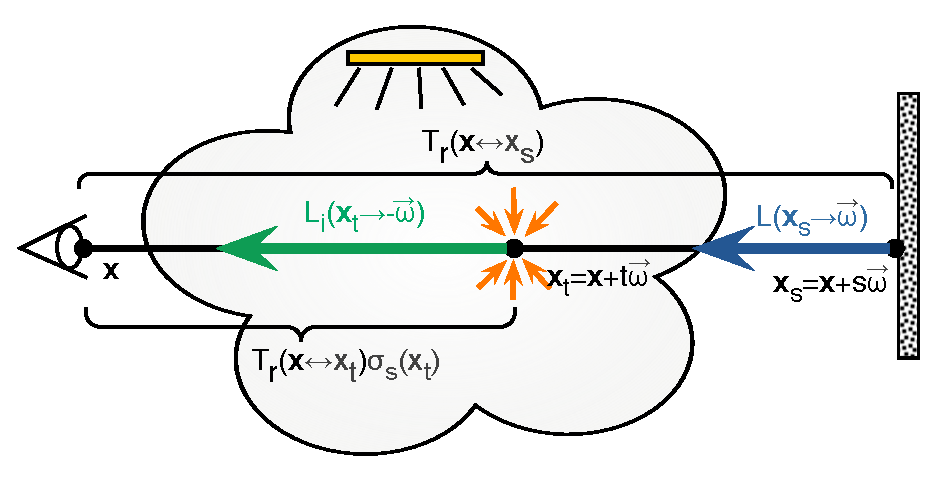
\includegraphics[width=\textwidth]{figures/pm/transmittance}
	\caption{参与介质被认为是一些微观散射粒子的组合,其物体几何形状为这些粒子所在体积的边界,当光线穿过这些介质时,其辐射亮度$L$会随着传输的距离而发生变化}
	\label{f:pm-transmittance}
\end{figure}

式\ref{e:pm-rte}表示的辐射传输的积分形式在计算机图形学中又称为体积渲染方程(volume rendering equation)\myindex{体积渲染方程}{volume rendering equation}。相交于4维(2D的表面位置及2D的球面坐标方向)的表面渲染方程,体积渲染方程是一个5维的方程:介质中3D的位置及其2D的(球面坐标)方向,并且光线在介质中每个位置处的辐射亮度都依赖于介质中其他所有位置,所以计算量非常复杂。在本书中我们将会介绍各种不同的方法用于体积渲染,其中本章介绍的光子映射是参与介质渲染最具吸引力的算法。





\subsection{体积光子映射}\label{sec:pm-volumetric-phptpn-mapping}
\cite{a:EfficientSimulationofLightTransportinSceneswithParticipatingMediausingPhotonMaps}对传统的光子映射算法进行了扩展,使其能够模拟光照在参与介质中的传输,新的算法称为体积光子映射(volumetric photon mapping)\myindex{体积光子映射}{volumetric photon mapping},本节将对其进行简单介绍,它是后面一些更高级方法的基础。体积光子映射涉及对光子追踪和光线追踪两个阶段的一些修改。



\subsubsection{光子追踪}
我们的目标是要生成一个符合光子在介质中传播特征(更确切地说,光子在介质中的传播受消光系数的影响)的一个光子分布图。在表面间的传输中,光子仅与表面发生交互而被记录到光子图中,但是光子在介质中的传播过程中,它可能与光线上的任意粒子发生交互,例如被吸收或散射,因此我们的目标便变成获得一个光子在介质中传输的距离值,使得光子在与任意粒子发生交互之前可以在该距离内自由传播,我们称这样的一个路径为自由路径(free-path)\myindex{自由路径}{free-path},获得这样一个自由路径的过程则称为自由路径采样(free-path sampling)\myindex{自由路径采样}{free-path sampling}。

很显然,根据重要性采样原理,我们希望这样的自由路径的距离分布是复合介质特征的,由于光子在介质中的传播过程中与粒子发生交互的几率取决于前面介绍的消光系数$\sigma_t$,而根据上一节的内容,透射比$T_r$实际上给出了一条光线在介质中两点之间无障碍传输的概率,因此我们可以对一条光线上\footnote{这里是指从光线起点开始,沿着其传播方向直到离开介质的整个光线片段部分,因为光子可能根据不同的概率与该片段上的任意位置处的粒子发生交互。}透射比$T_r$的分布来对自由路径进行采样,以产生一个光子,那么这样的光子分布图将是符合光子在该介质中的传输特征的,如图\ref{f:pm-volumetric-photon-tracing}所示。

\begin{figure}
	\sidecaption
	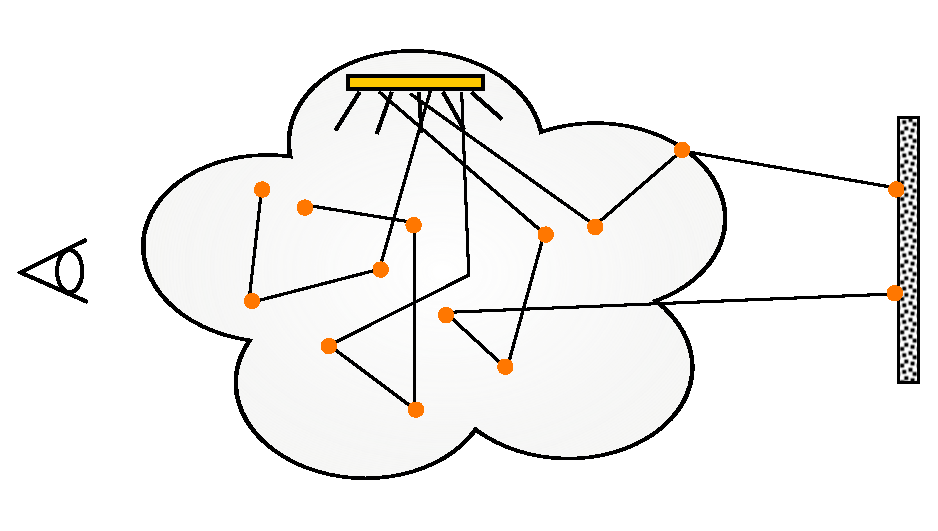
\includegraphics[width=0.55\textwidth]{figures/pm/volumetric-photon-tracing}
	\caption{在体积光子映射中,除了表面的光子,在介质中传播的光子还需要对每条光线的透射比进行采样得到一个与粒子进行交互的距离,从而在介质内产生一个光子,如果光子在采样距离处被散射,则对相位函数进行采样得到新的散射方向}
	\label{f:pm-volumetric-photon-tracing}
\end{figure}

例如对于同质介质,由于其消光系数为常数,其距离采样的概率密度函数可以表述为:

\begin{equation}
	{\rm pdf}(d)=e^{-\sigma_t(\mathbf{x})d}
\end{equation}

对于异质介质,可以通过求平均消光系数$\bar{\sigma}_t(\mathbf{x})$等方式来近似计算距离采样的概率密度函数。我们将在第\ref{sec:pm-transmittance-estimate}节详细讨论各种更高级的透射比估计方法。

当计算出光子与介质发生交互的位置之后,光子在该位置可能被散射或吸收,其各自发生的概率分别为$\sigma_s/\sigma_t$和$\sigma_a/\sigma_t$,这里使用俄罗斯轮盘(Russian roulette)\myindex{俄罗斯轮盘}{Russian roulette}进行选择即可;如果光子没有被吸收,则它会被散射到其他方向,该方向可以通过对其相位函数进行重要性采样得出。

在介质传输过程中生成的光子通常被存储在一个独立的体积光子图(volume photon map)\myindex{体积光子图}{volume photon map}中,如图\ref{f:pm-volumetric-photon-tracing}所示。






\subsubsection{光线步进及体积辐射亮度估计}
在表面之间的光照传输中,给定一个观察方向,光子映射算法只需要对沿该方向的光线与第一个(漫反射)表面的交点进行辐射亮度估计即可,然而对于参与介质内的光照传输,光线穿过介质的整个长度内都可能与介质中的粒子发生交互,从而得到来自向内散射的光照,因此我们需要对整条光线在介质内的部分执行光照计算,这样的计算成本非常昂贵,所以实践上我们常常使用光线步进(ray marching)\myindex{光线步进}{ray marching}来选取一些具有固定步长间隔的离散点来近似光线传输的结果,如图\ref{f:pm-vpm-ray-marching}所示,所以涉及参与介质的光照计算可以表述为:

\begin{equation}
\begin{aligned}
	L(\mathbf{x}\leftarrow\vec{\omega})\approx &T_r(\mathbf{x}\leftrightarrow\mathbf{x}_s)L(\mathbf{x}_s\to -\vec{\omega})\\ +&\Biggl(\sum^{S-1}_{t=0}T_r(\mathbf{x}\leftrightarrow\mathbf{x}_t)\sigma_s(\mathbf{x}_t)L_i(\mathbf{x}_t\to -\vec{\omega})\Delta_t\Biggl)
\end{aligned}
\end{equation}

其中,上式右边第一部分表示来自介质外的辐射亮度,该部分光照在介质中的传输受到透射比$T_r$的影响,通常入射光照$L(\mathbf{x}_s\to -\vec{\omega})$来自于该光线与表面的第一个交点(如图\ref{f:pm-vpm-ray-marching}中的$\mathbf{x}_s$点),其值通常使用表面光子映射计算而得;右边第二部分则是来自光线在介质内部的传输过程中各个位置$\mathbf{x}_t$处的向内散射贡献的光照,对于向内散射的辐射亮度$L_i(\mathbf{x}_t\to -\vec{\omega})$,则使用本节讨论的体积辐射亮度估计(volumetric radiance estimate)\myindex{体积辐射亮度估计}{volumetric radiance estimate}近似计算而得,与表面光子密度估计类似,它通过对点$\mathbf{x}_t$周围最近的$k$个光子进行概率密度估计而得(如图\ref{f:pm-vpm-ray-marching}所示):

\begin{equation}
	L_i(\mathbf{x},\vec{\omega})\approx\sum^{k}_{p=1}p(\mathbf{x}_t,\vec{\omega}\leftrightarrow\vec{\omega}_p) \cfrac{\Phi_p(\mathbf{x}\to-\vec{\omega}_p)}{\mathcal{V}(\mathbf{x})}
\end{equation}

\noindent 其值$\mathcal{V}(\mathbf{x})= \cfrac{4}{3}\pi d_k(\mathbf{x})^{3}$表示$k$个最近邻光子构成的球体积。

\begin{figure}
	\sidecaption
	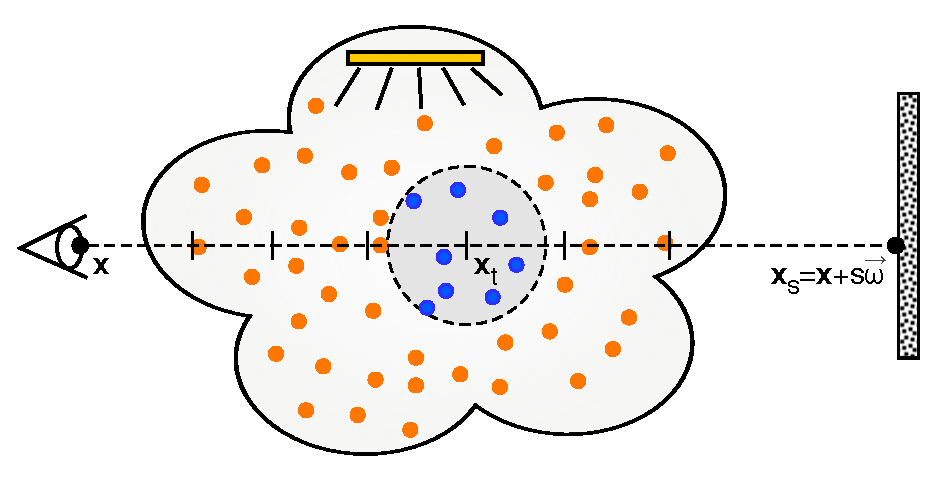
\includegraphics[width=0.65\textwidth]{figures/pm/vpm-ray-marching}
	\caption{体积光子映射使用光线步进的方式来收集光线传输过程中在介质内部的向内散射的光照,在每一个离散的点处,向内散射的辐射亮度使用体积辐射亮度估计计算而得}
	\label{f:pm-vpm-ray-marching}
\end{figure}





\subsection{光线图}\label{sec:pm-ray-maps}
上一节介绍的体积光子映射虽然仅对光子映射做少量的修改就能处理参与介质,然而由于介质内部到处都充满着光子,这种将传统表面的点采样(point sampling)\myindex{点采样}{point sampling}技术简单扩展到介质中则显得有些不合适。例如在光线步进的过程中,较小的步幅将增加光子图范围查询的计算量,而较大的步幅又会使得样本过少而呈现更多的噪点;另一方面,光线步进的方式也不是最优的:如果相邻步幅的球体存在重叠,则光子会被重复计算,如果步幅过大,则又容易漏掉一些可能包含重要信息的光子,如图\ref{f:pm-gathering-searches}所示。

\begin{figure}
	\sidecaption
	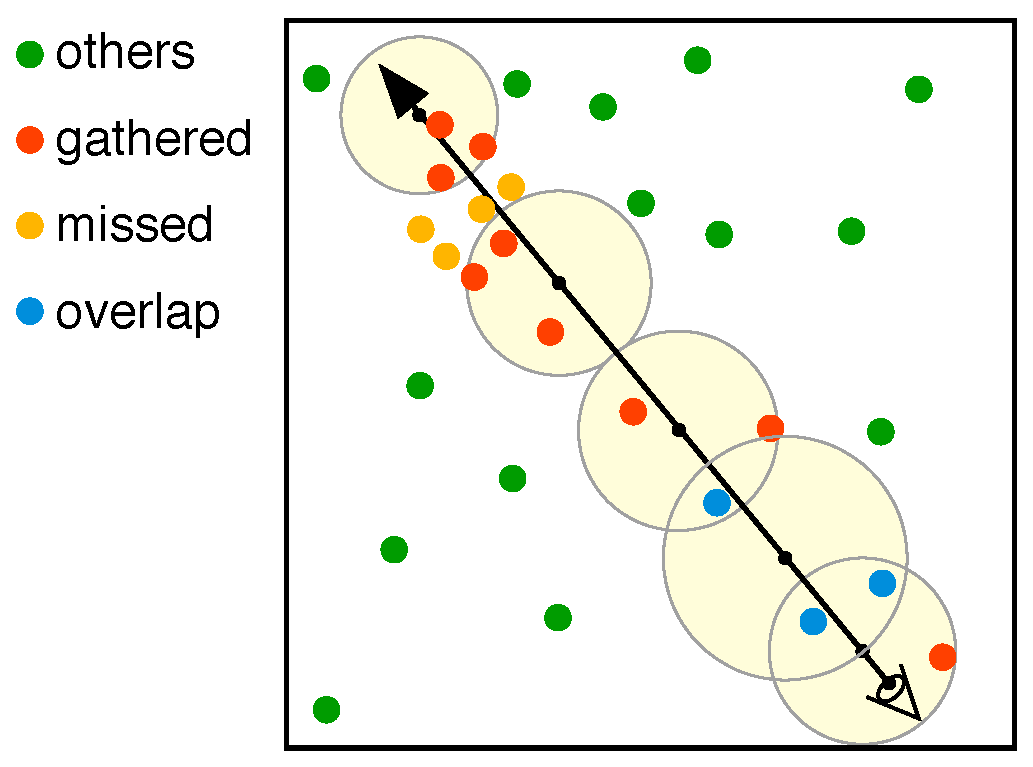
\includegraphics[width=0.52\textwidth]{figures/pm/gathering-searches}
	\caption{传统的体积光子映射通过光线步进的方式,在每个步幅处收集一个球体范围内的光子,这种方式可能导致重叠(蓝色)或者未命中(橙色)的光子}
	\label{f:pm-gathering-searches}
\end{figure}

上述体积光子映射的这些问题,其实源于传统的表面光子映射。当光子在表面之间进行传输时,对于每一条光线,它只包含唯一一个与表面的交点需要计算(或估计),因此这些表面间的全局光照技术都可以称之为是点采样(point sampling)\myindex{点采样}{point sampling},然而当光子在介质中传输时,需要对整个光线在介质中的部分进行积分,这是两种非常不同的传输模式,点采样是为表面间的光照传输设计的,生硬地将其扩展至介质中也许不是最好的方案。

从本节开始我们将讨论一种直接针对一条光线,而不是其中的某个点进行光照计算的思路,这些思路为光子在介质中的传输提供了一种全新的研究角度和计算模型。本节的光线图则是理解这些理论的基础。




\subsubsection{光子图的缺陷}
光线图(ray maps)\cite{a:RayMapsforGlobalIllumination}的提出源于弥补光子图(photon maps)的一些缺陷。由于光子图仅记录光照传输的结果,即最终落在表面上的一个光子,而不是光照传输的过程,即光线路径,最终我们仅能通过表面之间的接近度(proximity)来寻找这些光子,这直接导致了边界偏差(boundary bias)\myindex{边界偏差}{boundary bias},如图\ref{f:pm-biases}(b)所示,即在边界部分,实际参与估计的光子数量很少,而用于估计计算的面积却没变,这导致光照被过低估计(underestimation)\myindex{过低估计}{underestimation},例如一些线状类物体或者物体边缘会变暗。

\begin{figure}
	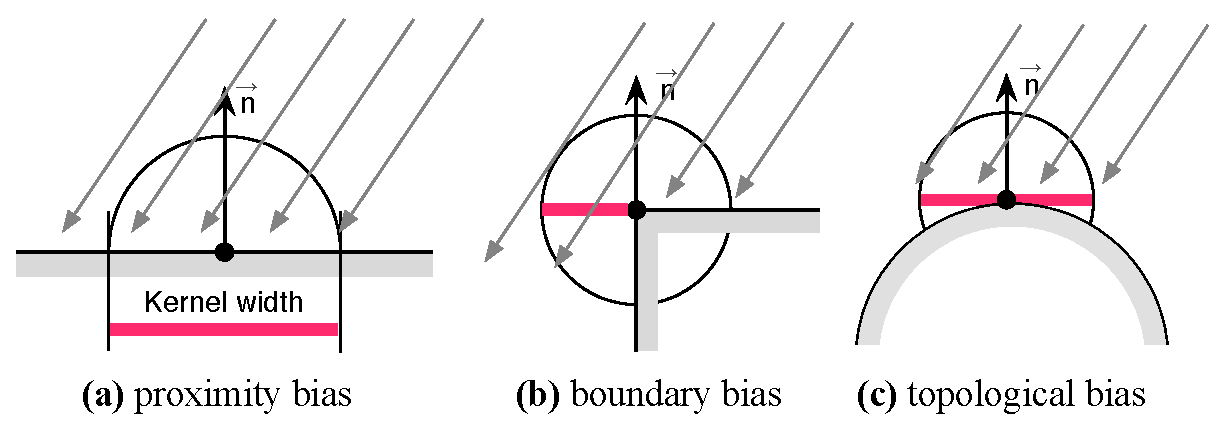
\includegraphics[width=\textwidth]{figures/pm/biases}
	\caption{光子密度估计的三种偏差来源:(a)核估计导致的偏差,(b)物体边缘由于几何形状导致被过低估计的偏差,以及(c)局部非平坦拓扑面形成的过高估计的拓扑偏差}
	\label{f:pm-biases}
\end{figure}

怎样才能减小这类偏差呢?显然通过比较精确地匹配参与估计的光子及其实际对应的面积(或体积)是非常困难的,这也是我们一般使用圆形等简单几何形状来描述核函数的原因。通过观察图\ref{f:pm-biases}可以看出,如果我们对估计点附近的光线(rays)而不是其落在表面上的光子(photon)进行估计,则其结果会更为准确,这就要求我们记录每个光子对应的光线,而不是仅仅是光子的光照值本身。

\cite{a:AParticlePathbasedMethodforMonteCarloDensityEstimation}第一次从概念和方法上提出了使用光线来进行光子密度估计的方法,它同时记录每个光子所在的光线,然后使用最近的$k$个与估计点$\mathbf{x}$的正切面相交的光线来进行概率密度估计,这样表面上最近邻的光子搜索转换为光线-圆盘相交(ray-disc intersection)\myindex{光线-圆盘相交}{ray-disc intersection}测试,如图\ref{f:pm-ray-disc}所示。通过光线来进行光子密度估计不仅能够消除边界偏差,并且该方法并不依赖于物体的尺寸,甚至它不要求物体局部是平坦的,因为正切面上的圆盘是独立于其局部几何形状的。

\begin{figure}
	\sidecaption
	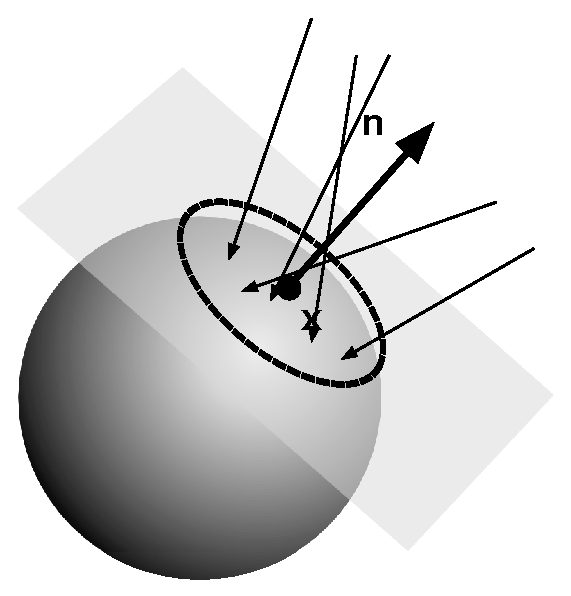
\includegraphics[width=0.4\textwidth]{figures/pm/ray-disc}
	\caption{\cite{a:AParticlePathbasedMethodforMonteCarloDensityEstimation}通过记录每个光子所在的光线,然后通过这些光线与表面$\mathbf{x}$处周围一个圆面进行光线-圆面的相交计算来确定待估计的光子,这减少了边界偏差}
	\label{f:pm-ray-disc}
\end{figure}

\cite{a:RayMapsforGlobalIllumination}在此基础上提出了更加完善的光子图(ray maps)的理论,下面我们将详细介绍相关的算法,数据结构以及对应的一些思路。




\subsubsection{光线近邻查询}
光线图记录了场景中所有光线片段的索引值(我们将在后面介绍光线图的数据表述),然后这些索引值便可以被用于查询如:经过空间中任意一点附近的光线,以及经过一个物体边界范围(boundary)的所有光线,且这些查询操作是完全独立于这些光线对应的光子与查询点实际的几何距离的,例如在图\ref{f:pm-biases}(b)中,那些光子的距离不在近邻范围,但是其所在的光线却穿过查询点的近邻范围时,该光子仍然参与了估计,因此边界偏差被完全消除。

\begin{figure}
\sidecaption
	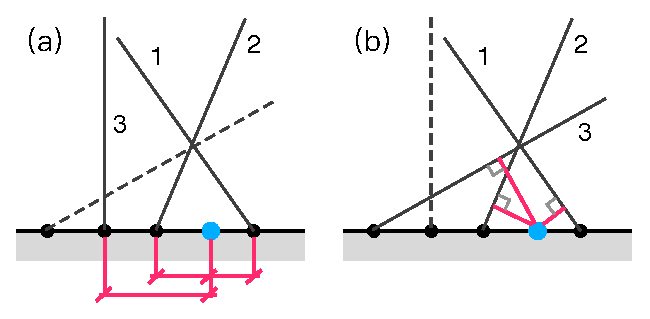
\includegraphics[width=.65\textwidth]{figures/pm/ray-proximity-queries}
	\caption{不同距离度量下的3个光子的最近邻查询:(a)到光线与正切面交点的距离,(b)查询点到光线的垂直距离。可以看到不同的距离度量具有各自的优点,(a)强调了光子在距离上的近邻性,而(b)强调了光线在空间上的相邻性}
	\label{f:pm-ray-proximity-queries}
\end{figure}

\cite{a:RayMapsforGlobalIllumination}定义了两种不同类型的对光线近邻查询(ray proximity queries)\myindex{光线近邻查询}{ray proximity queries}操作:即相交点查询(intersection queries)\myindex{相交点查询}{intersection queries}和最近邻查询(nearest neighbor queries)\myindex{最近邻查询}{nearest neighbor queries}。相交点查询是指查询与某个固定尺寸大小的空间区域(spatial domain)\myindex{空间区域}{spatial domain}相交的所有光线,而最近邻查询是指查找某个给定距离度量下的$k$个最近邻光线,其中每种查询可以使用不同的空间域和距离度量:

\begin{enumerate}[label=\Roman*.]
	\item \textbf{相交点查询}\\
		使用不同的空间区域:(a)圆盘面(disc),(b)半球空间(hemisphere),(c)球体空间,(d)与坐标轴对齐的包围盒。
	\item \textbf{最近邻查询}\\
		使用不要的最近邻距离度量:估计点到(a)光线与正切面的交点的距离,(b)光线线段的垂直距离,(c)光线辅助线与正切面交点的距离。
\end{enumerate}

上述的查询操作通常可以联合起来使用,例如首先通过相交点查询来筛选潜在可能的最近邻光线,然后通过最近邻距离查询来得到具体对应的光线;或者例如后面介绍的使用其中一些距离度量来查询光线,而使用另一些距离度量的查询结果来作为核函数的权重系数计算依据。此外,根据上述的分类,\cite{a:AParticlePathbasedMethodforMonteCarloDensityEstimation}可以看做是使用\Romannum{2}.(a)的距离度量进行最近邻查询。




\subsubsection{光线图的表述}\label{sec:pm-ray-maps-data}
我们已经讨论了存储光线而不是光子的必要性,以及常用的对光子图的操作,这样我们能够理解使用何种数据结构存储光线图会使得查询更加高效。

在光子图中,每条光线就是一条完整路径中的每个线段(line segment),它记录了每个光线的起点,方向,长度等基本信息,此外它还包含一些其他信息用于辐射亮度估计的计算,算法\ref{a:pm-photon-beam}给出了一条光线的定义。

我们的目标是要寻找距离某个位置最近的光线\footnote{除了点查询,在本章后面光束相关的内容中,还将看到光线图(在那里称为光束)被用于沿着另一条光线查询,以及需要识别光线与某个区域相交的部分,而不仅仅是相交,所以后面还将看到根据不同的操作需要使用不同的数据结构。},\cite{a:RayMapsforGlobalIllumination}使用了基于空间细分的k-d树数据结构,每个非叶节点对空间进行划分,每个节点维护着一个与该部分空间相交的光线的列表。当进行相交点查询时,首先检查各个节点是否与给定空间域相交,然后在叶节点则比较每条光线是否与给定空间域相交;当进行最近邻查询时,首先选择最近的非叶节点,然后再确定遍历叶节点中的光线寻找距离最近的$k$条光线。相关的一些k-d树的遍历思路和上一章讨论的内容是相似的。




\subsubsection{光线图密度估计}
\cite{a:RayMapsforGlobalIllumination}使用了一种组合的最近邻查询方式,这种方法称为半球-盘面相交(hemisphere-disc intersection)方法。在该方法中,一条光线被选择必须同时满足以下条件:

\begin{enumerate}
	\item 光线必须与估计点周围半径为$R$的球形空间相交,即\Romannum{2}.(b),以及
	\item 光线本身或者光线的延长线(辅助线)与估计点正切空间的一个盘面相交,即\Romannum{2}.(a)
\end{enumerate}

图\ref{f:pm-hemisphere-disc}显式了几种不同的相交情形,光线1是标准的情况;光线2与表面的交点即使超出球面空间,但是仍然被包含在内;光线3不与正切面相交,但是其延长线与盘面相交;光线4虽然与球体相交,但是其延长线与正切面的交点没有落于盘面内;需要注意的是,光线7实际上被遮挡了,但是这里没有处理这种情况,所以当做标准情形处理了。

\begin{figure}
	\sidecaption
	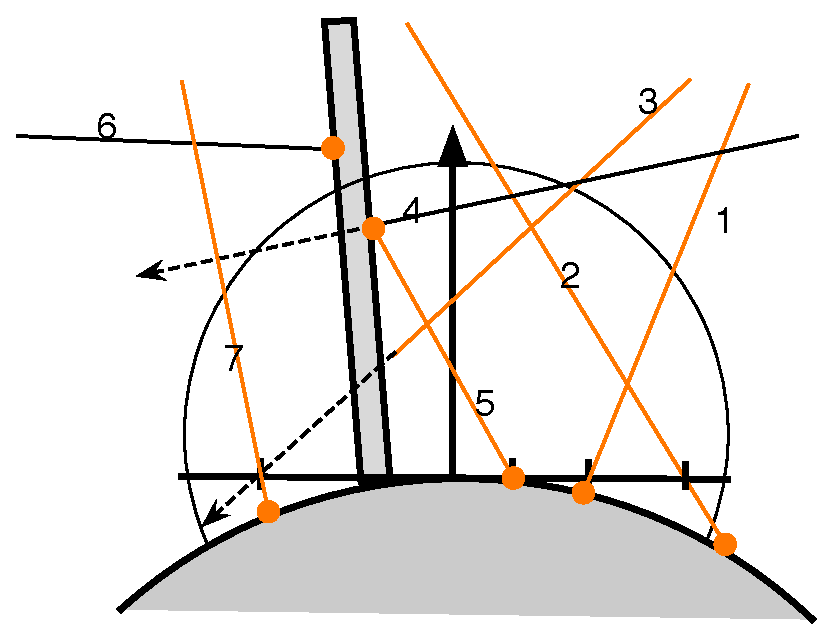
\includegraphics[width=0.6\textwidth]{figures/pm/hemisphere-disc}
	\caption{半球-盘面相交使用两个光线近邻查询的组合,即光线必须同时落于半径为$R$的球体范围内,以及光线本身或其延长线与正切面的交点落于盘面内}
	\label{f:pm-hemisphere-disc}
\end{figure}

当然上述方法知识一个启发式方法,它并不总能保证最优的结果,但是它比单纯使用正切盘面的方法\cite{a:AParticlePathbasedMethodforMonteCarloDensityEstimation}要好得多。首先,该方法和传统使用盘面的光子映射算法一样是一致的;其次,通过在空间对光线进行最近邻查找,而不是在物体表面对光子进行查找,这完全消除了边界偏差(如图\ref{f:pm-biases}(b)所示);最后,因为只有与正切盘面相交的光线才被考虑,这避免了落于拓扑结构较复杂的区域(如图\ref{f:pm-biases}(c)所示),这减少了拓扑偏差;此外,通过同时要求光线落于球体区域以及与正切盘面相交,这剔除了大部分空间上与待估点相邻,但是却不能贡献光照的光线,例如图\ref{f:pm-hemisphere-disc}中的光线4,这也减小了方差。

最后,半球-盘面相交发使用待估点距离光线本身或其延长线与正切盘面交点的距离作为密度估计核函数的权重计算依据。






\subsection{基于光束的光子映射}
传统的光子映射仅保存(通过某种自由路径采样)发生散射事件位置处的光子,而忽略光子追踪过程中累积的一些其他重要信息,例如在图\ref{f:pm-points-vs-beams}(a)中,由于估计点球形区域内不包含任何光子,因此其来自向内散射的光照贡献为0,这种情况下我们不得不使用更多的光子或者增加估计的半径,前者带来了内存压力以及光子密度估计的计算量,而后者则增加了偏差。

上一节讨论的光线图(ray maps)\myindex{光线图}{ray maps}则给了我们一个重要启示:如果在介质中存储整个光子的路径,则可以使用更少的光线来表述光照,并且大大增加了光子数据的密度,如图\ref{f:pm-points-vs-beams}(b)所示,估计点范围内虽然不包含任何发生散射的光子(点),但是它与两条光线相交,因此可以获得其相交部分光线的向内散射(in-scattering)\myindex{向内散射}{in-scattering}光照贡献。

\begin{figure}
	\sidecaption
	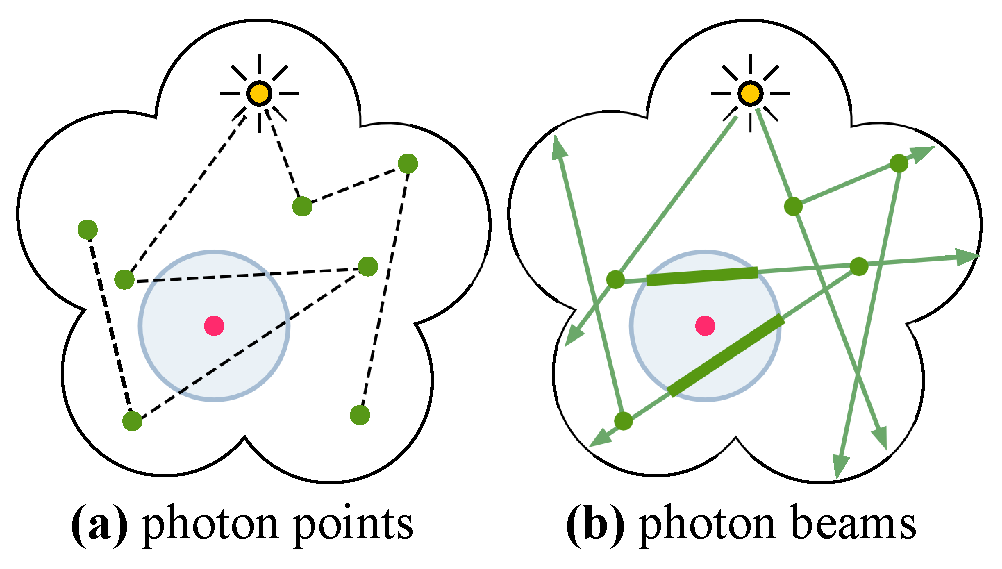
\includegraphics[width=0.65\textwidth]{figures/pm/points-vs-beams}
	\caption{传统的体积光子映射(a)存储所有发生散射事件的点,然后使用这些点进行密度估计;而光子束(b)则存储整个光子的轨迹(一些线段),然后使用这些线段进行密度估计。光子束大大增加了辐射亮度估计的质量,因为介质中线段占据的空间更多,“光子”密度更高}
	\label{f:pm-points-vs-beams}
\end{figure}

当然,在上一节中,光线图仅用于表面点的辐射亮度估计,光线的作用仅仅是用来减少边界偏差和拓扑偏差(如图\ref{f:pm-biases}所示),每条光线最终只被计入一个光子进行估计。然而当光线被扩展到介质中时,由于理论上介质中每个点都可能发生散射,因此其不仅被用于增加光子估计的密度,光线与估计区域相交的整个线段都对估计点具有光照贡献,这使得估计的质量大大提高。

另一方面,\cite{a:TheBeamRadianceEstimateforVolumetricPhotonMapping}将光线的概念运用于摄像机光线(而不是光子路径),通过直接对一条穿过介质的摄像机光线进行估计,而不是通过光线步进的方式来计算该条线段上有限的向内散射点的值,大大提高了渲染质量和计算效率。

光线的引入,为体积渲染提供了一种全新的算法基础,它有别于传统表面渲染中使用的点采样(point sampling)的方法,\cite{a:AComprehensiveTheoryofVolumetricRadianceEstimationusingPhotonPointsandBeams}在此基础上提出了一个完全基于线段的密度估计框架,这成为当前乃至以后体积渲染领域最主要的基础架构之一,以下我们将详细讨论基于光线的体积渲染。





\subsubsection{几何设定}
\cite{a:AComprehensiveTheoryofVolumetricRadianceEstimationusingPhotonPointsandBeams}提出了一个基于点和光线的统一框架,在新的框架下,传统的基于点采样的体积光子映射是其中一种特殊形式。

摄像机子路径和光源子路径都可以使用点(point)或者光束\footnote{从本节起,我们将称一条光线(ray)或一个线段(line segment)为光束。}(beam)的形式进行表述,这里称摄像机子路径的表述为查询表述(query representation)\myindex{查询表述}{query representation},它表示了要进行估计的量(例如对单个点进行估计,或者对一整条光束进行估计),称光源子路径的表述为数据表述(data representation)\myindex{数据表述}{data representation},它表示了平衡状态下光照的表述形式(例如以点的形式表述,或者以光束的形式表述),再加上每个估计方法可以使用不同的核估计函数(例如3D,2D或者1D的核估计函数),我们可以按data$\times$query(kernel)的组合来唯一区分一个估计方法,\cite{a:AComprehensiveTheoryofVolumetricRadianceEstimationusingPhotonPointsandBeams}一共提出了9种独立的估计方法,如图\ref{f:pm-estimators}所示。

为了使将注意力集中于不同路径表述形式下的辐射亮度估计部分,我们将完整路径的其他部分做一些简化,这里遵循\cite{a:UnifyingPointsBeamsandPathsinVolumetricLightTransportSimulation}中使用的定义及设定。图\ref{f:pm-estimators}(a)表示了所有估计形式的共享的几何设定部分,设一条光源子路径的第$s$个顶点为$\mathbf{x}_{s-1}\equiv \mathbf{a}$,对$\mathbf{a}$点的反射系数进行采样得到一个方向$\omega_{\mathbf{a}}$,则光线$(\mathbf{a},\omega_{\mathbf{a}})$定义了一个光子光束(photon beam)\myindex{光子光束}{photon beam},则该光束的能量可以表述为该子路径的权重\footnote{注意,为了便于后面的表述,本节中涉及的路径能量都被除于采样概率了,因此称为路径权重(path weight)\myindex{路径权重}{path weight};例如这里在$\mathbf{a}$点的散射其光照贡献为散射系数$\rho(\mathbf{a})$,但是这里除于了对应的概率密度,因此其结果就对应于蒙特卡洛估计中被平均前的每一项的值,即$ \cfrac{f(x)}{p(x)}$。}(weight)乘以$\mathbf{a}$点处的反射系数:

\begin{equation}
	C_l(\mathbf{x}_0\cdots\mathbf{a}]=C_l(\mathbf{x}_0\cdots\mathbf{a}) \cfrac{\rho(\mathbf{a})}{p(\omega_{\mathbf{a}})}
\end{equation}

同理,设摄像机子路径的顶点$\mathbf{x}_{s+1}\equiv\mathbf{c}$,并对$\mathbf{c}$点的散射系数进行采样得到方向$\omega_{\mathbf{c}}$,则光线$(\mathbf{c},\omega_{\mathbf{c}})$定义了一条查询光束(query beam)\myindex{查询光束}{query beam},相应地,该光束的能量可以表述为:

\begin{equation}
	C_e(\mathbf{c}\cdots\mathbf{x}_k]= \cfrac{\rho(\mathbf{c})}{p(\omega_{\mathbf{c}})}C_e(\mathbf{c}\cdots\mathbf{x}_k)
\end{equation}

通过沿光线$(\mathbf{a},\omega_{\mathbf{a}})$的方向采样\footnote{这里的距离需要对前面介绍的透射比$T_r$采样而得,也就是自由路径采样,它表示光子能够无障碍达到点$\tilde{\mathbf{b}}$的概率。}得到一个距离$t_{\mathbf{a}}$,我们可以在光子光束$(\mathbf{a},\omega_{\mathbf{a}})$上的位置$\tilde{b}\equiv\tilde{\mathbf{x}}_s$处创建一个光子,该光子的权重为$C_l(\mathbf{x}_0\cdots\mathbf{a}] \cfrac{T_r(t_a)}{p(t_a)}$;同理,通过沿着查询光束$(\mathbf{c},\omega_{\mathbf{c}})$采样得到一个距离$t_{\mathbf{c}}$,可以在未知$\mathbf{b}\equiv\mathbf{x}_s$处创建一个查询点(query point)\myindex{查询点}{query point},其权重为$ \cfrac{T_r(t_c)}{p(t_c)}C_e[\mathbf{c}\cdots\mathbf{x}_k)$。

上述的基本设定适用于以下将讨论的所有估计,即所有的估计共享相同的前缀$C_l(\mathbf{x}_0\cdots\mathbf{a}]$及后缀$C_e(\mathbf{c}\cdots\mathbf{x}_k]$,因此我们将在表述中省略这两部分以简化估计公式;这里的散射函数$\rho$是包含消光系数$\sigma_s$的,参见式\ref{e:pm-scattering};所有的估计类型按照数据表述(\textbf{P}oint/\textbf{B}eam)-查询表述(\textbf{P}oint/\textbf{B}eam)以及核函数的维度(1D,2D或3D)进行区分,例如B-P3D表示beam data$\times$ point query, 3D kernel,如图\ref{f:pm-estimators}(e)所示。
	
\begin{figure}
\begin{fullwidth}
	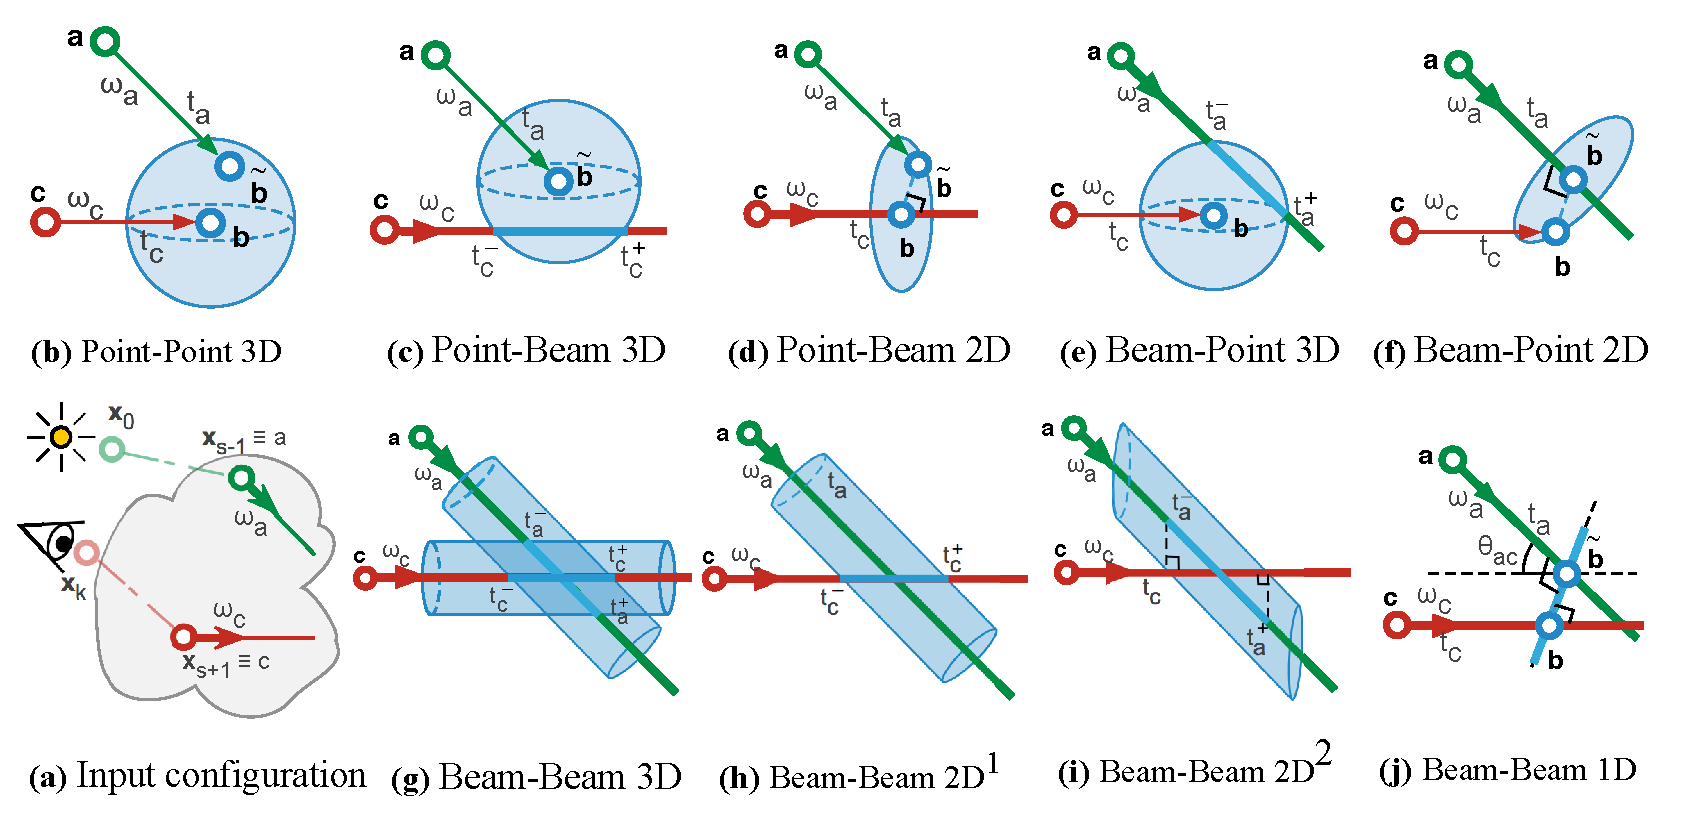
\includegraphics[width=1.0\thewidth]{figures/pm/estimators}
	\caption{\cite{a:AComprehensiveTheoryofVolumetricRadianceEstimationusingPhotonPointsandBeams}提出的9种体积辐射亮度估计,这里使用Data-Query(Kernel)的形式,注意较粗的路径表示度量为光束,需要考虑透射比的作用,而较细的路径表示度量为点,它们通常还需要通过对查询光线的某种自由路径采样来计算整条光束的光照值;例如(d)表示对一条光束进行估计,而(e)表示对路径上一个点进行估计;蓝色粗线表示需要对向内散射进行积分计算以求光子经过一段距离(通常是查询表述和数据表述相交的区域)获得的向内散射光照。}
	\label{f:pm-estimators}
\end{fullwidth}
\end{figure}


以下,我们将从最基本的Point-Point 3D(这也对应于传统的体积光子映射)的估计开始逐个推导,介绍它们在各个步骤上和传统点采样方法区别和思路,以及各个估计之间的一些内在联系,在后面我们将分析这些估计在处理不同属性介质时效率上的差异,因此第\ref{sec:pm-upbp}将介绍怎样使用复合重要性采样将这些估计组合起来形成更高效的采样方法。




\subsubsection{基于光子点的辐射亮度估计}
本节我们将首先讨论最简单的情形,即将数据表述限定为光子点的形式,推导出直接对一条查询光束进行辐射亮度估计的公式,即是\cite{a:TheBeamRadianceEstimateforVolumetricPhotonMapping}中的光束辐射亮度估计。



\paragraph{Point-Point 3D估计}
传统的体积光子映射通过在一个查询点附近搜索光子来对向内散射辐射亮度进行估计,如图\ref{f:pm-estimators}(b)所示,由于我们的几何设定中输入配置为一条光子光束和一条查询光束,因此这里 为了产生光子和查询点,还需要对光子光束和查询光线使用一个自由路径采样,对查询点搜索到的近邻光子使用一个3D的核函数得到的估计如下:

\begin{equation}\label{e:pm-pp3d}
	\langle I\rangle_{P-P3D}=\underbrace{ \cfrac{T_r(t_a)}{p(t_a)}}_{\text{photon sampling}}\rho(\tilde{\mathbf{b}},\mathbf{b})K_3(\tilde{\mathbf{b}},\mathbf{b})\underbrace{ \cfrac{T_r(t_c)}{p(t_c)}}_{\text{query point sampling}}
\end{equation}

注意上式仅包含单个(而不是整个搜索范围内的所有)光子的估计,这样的形式更便于后面复合重要性采样的需要,因为同一查询点搜索到的所有光子可能都来自于不同长度的光源子路径,因此其与查询点组成的全路径具有不同的路径长度,需要和各自对应路径长度的估计进行复合,而直接计算所有光子的估计结果则使得无法进行复合重要性采样。




\paragraph{Point-Beam 3D估计}
在上式的估计中, 为了计算查询光束$(\mathbf{c},\omega_{\mathbf{c}})$上所有的向内散射的光照,传统的做法(见第\ref{sec:pm-volumetric-phptpn-mapping}节)通常对查询光束使用光线步进的方法获取一些离散的查询点,然后对每个点分别使用式\ref{e:pm-pp3d}进行估计。这种做法使得每个查询点都需要对所有光子做一次最近邻搜索,增加了计算开支,与此相反,\cite{a:TheBeamRadianceEstimateforVolumetricPhotonMapping}提出光束辐射亮度估计(beam radiance estimate)\myindex{光束辐射亮度估计}{beam radiance estimate}的概念,它直接对一条查询光束进行估计,这样每条光线对所有光子只进行一次最近邻查询操作。

通过图\ref{f:pm-estimators}(c)的图示不难看出,由Point-Point 3D转变为Point-Beam 3D实际上就是将式\ref{e:pm-pp3d}中单个查询点的采样$ \cfrac{T_r(t_c)}{p(t_c)}$转变为一个从$t^{-}_c$到$t^{-}_c$积分,由于每个查询点都需要做一次最近邻搜索,所以被积函数应该包含光子点,即:

\begin{equation*}
	\langle I\rangle_{P-B3D}={\rm \int}^{t^{+}_{c}}_{t^{-}_{c}}\underbrace{ \cfrac{T_r(t_a)}{p(t_a)}}_{\text{photon sampling}}\rho(\tilde{\mathbf{b}},\mathbf{b}_{t_c})K_3(\tilde{\mathbf{b}},\mathbf{b}_{t_c})T_r(t_c){\rm d}t_c
\end{equation*}

不幸的是,由于光子点被包含在了被积函数中,使得上式的计算非常复杂。但是我们可以从其对偶视角(dual perspective)\myindex{对偶视角}{dual perspective}来进行分析:即将每个光子看做3D核估计体积的中心,如果每个光子与查询光束相交,则计算其对整条查询光束的光照贡献,此种视角下每个光子相对于整个查询光束的积分是一个常数,所以我们可以将光子点从被积函数中抽取出来,形成如下的估计:

\begin{equation}\label{e:pm-pb3d}
	\langle I\rangle_{P-B3D}=\underbrace{ \cfrac{T_r(t_a)}{p(t_a)}}_{\text{photon sampling}}{\rm \int}^{t^{+}_{c}}_{t^{-}_{c}}\rho(\tilde{\mathbf{b}},\mathbf{b}_{t_c})K_3(\tilde{\mathbf{b}},\mathbf{b}_{t_c})T_r(t_c){\rm d}t_c
\end{equation}

在上述的估计中,对于每一条查询光束,我们仅需要对所有光子遍历一次,$t^{-}_c$到$t^{+}_c$是每个光子的3D核估计体积与查询光束相交的部分,它可以简单地通过光线-球体相交(ray-sphere intersection)\myindex{光线-球体相交}{ray-sphere intersection}测试计算而得,如图\ref{f:pm-estimators}(c)所示。

\begin{figure}
	\sidecaption
	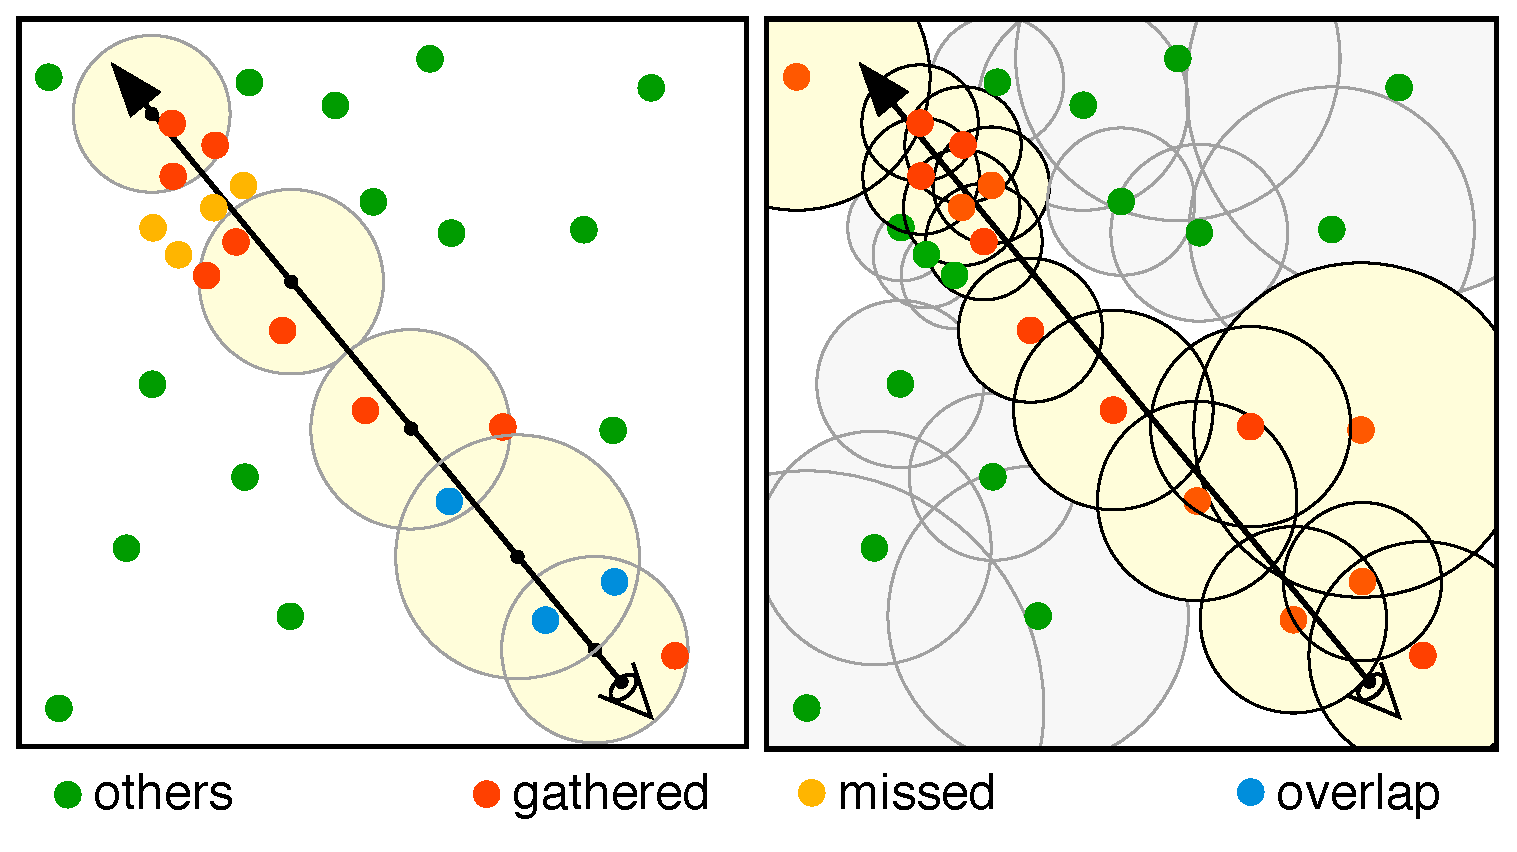
\includegraphics[width=0.65\textwidth]{figures/pm/beam-gathering}
	\caption{基于查询光束的光子估计能够通过仅对所有光子遍历一次来提升计算效率,并且通过能够包含所有与查询光束相交的光子来提升渲染质量及收敛速度}
	\label{f:pm-beam-gathering}
\end{figure}

图\ref{f:pm-beam-gathering}展示式\ref{e:pm-pb3d}(右边小图)与式\ref{e:pm-pp3d}(左边小图)的区别(注意,由于式\ref{e:pm-pp3d}仅表示单个查询点的估计,所以这里使用传统的光线步进来计算整条查询光线的光照),从这里可以看到式\ref{e:pm-pb3d}能够避免对光子的重复计算,每个光子仅被查询一次,大大减少了光子查询的计算量;此外,基于查询光束的估计能够考虑全部对查询光束有贡献的光子,而传统的光线步进的方法则容易漏掉一些光子。



\paragraph{Point-Beam 2D估计}
式\ref{e:pm-pb3d}虽然减少了对光子的重复搜索操作,但是对于每个光子,它仍然需要在光子球体与查询光束相交的区域,即$t^{-}_{c}$到$t^{+}_{c}$的区域做积分运算,这个计算大大影响了估计的效率。\cite{a:TheBeamRadianceEstimateforVolumetricPhotonMapping}进一步提出了一个近似方法用于计算式\ref{e:pm-bp3d}。

观察式\ref{e:pm-bp3d},可以假设在局部范围内,$\rho(\tilde{\mathbf{b}},\mathbf{b}_{t_c})$的变化很小,因此可以进行将其抽取到积分外,而$K_3(\tilde{\mathbf{b}},\mathbf{b}_{t_c})$也是一个常数(因为这里的概率密度估计只计算落入估计范围内光子的数量),因此积分部分被简化为仅在$t^{-}_{c}$到$t^{+}_{c}$的区域对透射比$T_r(t_c)$进行积分,如图\ref{f:pm-averaging-transmittance}(a)所示。

\cite{a:AComprehensiveTheoryofVolumetricRadianceEstimationusingPhotonPointsandBeams}指出,由于这里的密度估计对于核函数的几何形状是没有限制的,因为我们仅计算落入估计范围的光子数量,因此我们可以使用一个围绕光线的圆柱形来作为核函数的范围,其长度为$h=t^{+}_c-t^{-}_c$,半径与原球形核函数的半径相等,如图\ref{f:pm-averaging-transmittance}(b)所示,则此时透射比沿$t^{-}_{c}$到$t^{+}_{c}$的积分值除以该区域的长度等于该区域的平均透射比,由此此时的圆柱形体积为$\pi r^{2}h$,$h$被用作平均计算之后还剩$\pi r^{2}$,它刚好是一个以$r$为半径的2D核函数。所示式\ref{e:pm-bp3d}可以近似为:

\begin{equation}\label{e:pm-pb2d}
	\langle I\rangle_{P-B2D}=\underbrace{ \cfrac{T_r(t_a)}{p(t_a)}}_{\text{photon sampling}}\rho(\tilde{\mathbf{b}},\mathbf{b})K_2(\tilde{\mathbf{b}},\mathbf{b})T_r(t_c)
\end{equation}

上式使用了一个2D的核估计,但是式\ref{e:pm-bp3d}中的积分项被去掉,而被一个平均透射比代替,当估计的半径越来越小时,$\lim{h}=0$时,式\ref{e:pm-bp3d}越来越接近于式\ref{e:pm-bp2d},但是后者的计算要高效的多。

\begin{figure}
	\sidecaption
	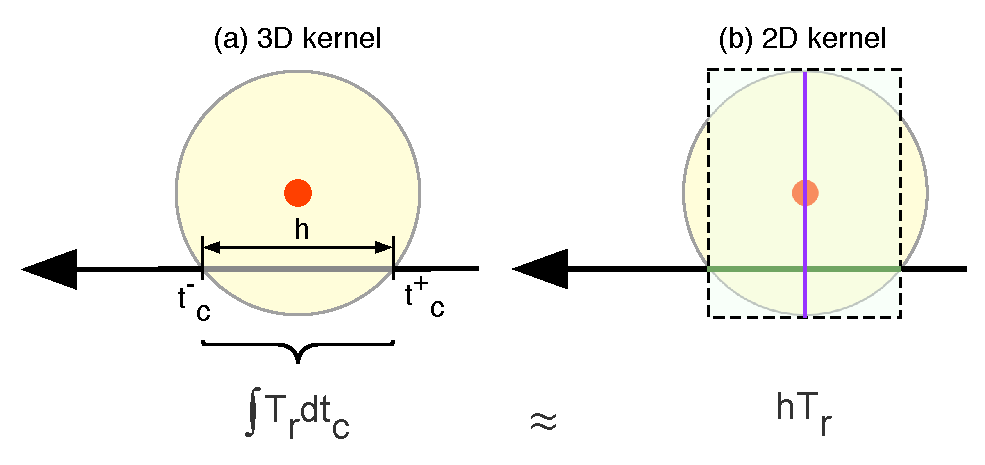
\includegraphics[width=0.65\textwidth]{figures/pm/averaging-transmittance}
	\caption{通过平均透射比来代替透射比的积分,可以将更高维度的核函数进行降维,这里圆形区域为2D核函数,紫色线段表示1D核函数;其转换的关键是概率密度估计与核函数形状无关}
	\label{f:pm-averaging-transmittance}
\end{figure}

通过降维来计算积分的平均值,这避免了复杂的积分计算,这是本节及后续估计会使用的重要方法和手段,也是基于光束的体积渲染实现计算效率提升的关键。





\paragraph{光子的表述}
与传统光子映射使用k-d树对光子进行最近邻搜索不同的是,本节介绍的光束辐射亮度估计通过对偶视角来看待光子密度的估计,搜索半径直接附加在了每个光子身上,因此搜索问题转变成光线-球体相交(ray-sphere intersection)\myindex{光线-球体相交}{ray-sphere intersection}计算,这需要一种新的表述光子的数据结构。

\cite{a:TheBeamRadianceEstimateforVolumetricPhotonMapping}使用了包围盒层次结构(bounding-box hierarchy)来存储光子数据,其算法包含如下几步:

\begin{enumerate}
	\item 使用传统的光子追踪从光源产生平衡态下的光子分布。
	\item 将所有光子构建为一个k-d树以满足下一步的最近邻查询需求。
	\item 对每个光子执行最近邻搜索以产生搜索半径。
	\item 为每个光子构建一个能够包围搜索半径的包围盒。
	\item 根据每个光子的包围盒边界构建包围盒层次机构。
\end{enumerate}

上述过程构建的BBH结构将用于光子与查询光束的相交测试,由此也可以看出,基于光束的辐射亮度估计很自然地支持适应性的核估计带宽。当然,如果我们只是对所有光子使用固定带宽,则不需要对光子构建k-d树,或者也可以使用光子微分来计算每个光子使用的带宽。

\begin{figure}
	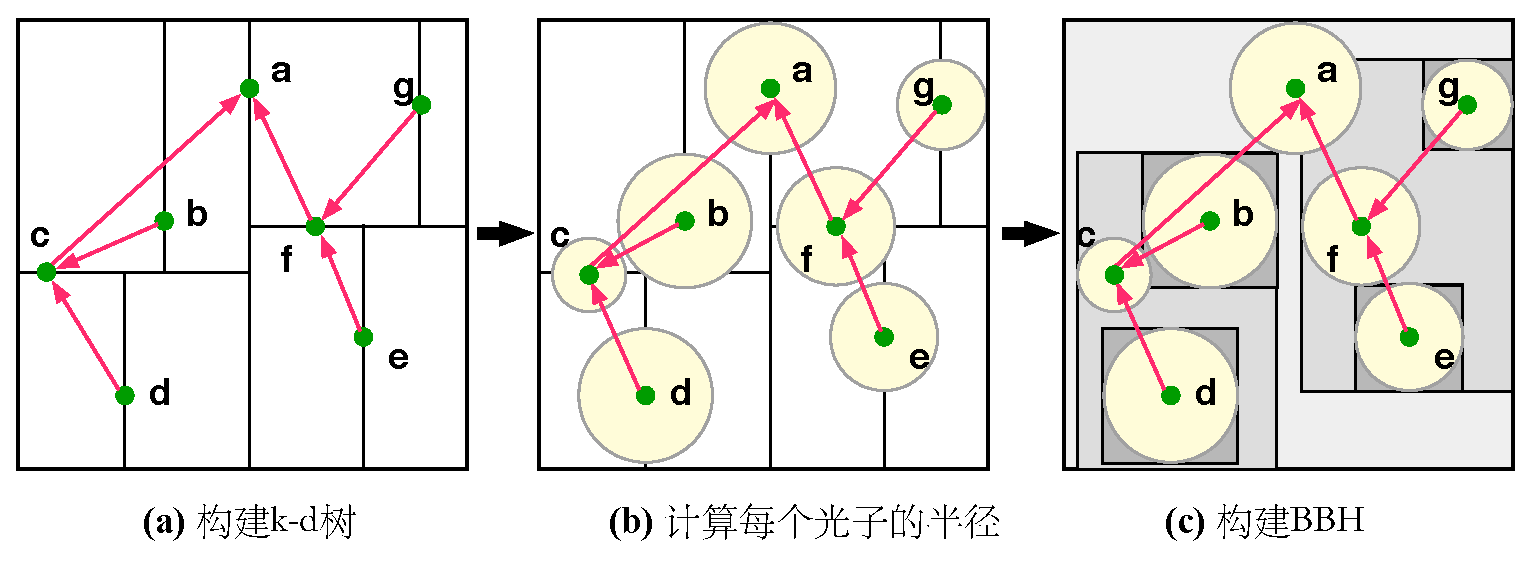
\includegraphics[width=1.0\textwidth]{figures/pm/bbh}
	\caption{在光子被生成之后,首先对光子构建一个k-d树(a),该k-d树被用于执行最近邻查询一计算每个光子的带宽(b),最后以每个光子的带宽为边界构建一个包围盒层次结构(c),注意这里包围盒层级结构和k-d树具有相同的层级结构,如图中的红色箭头所示}
	\label{f:pm-bbh}
\end{figure}



\subsubsection{基于光子光束的辐射亮度估计}
上一节将光束的概念运用于摄像机子路径,直接对一条查询光束(而不是单个查询点)进行估计,它减少了光子重复搜索的计算量,并且通过一些近似方法大大简化了复杂的积分计算,本节我们将相似的概念扩展到光源子路径。

不同于摄像机子路径的是,光源子路径的每一条路径线段都可能对估计产生贡献,而摄像机子路径只需要考虑最后一条光束(即是通过介质的光束),因此光子光束(photon beam)\myindex{光子光束}{photon beam}需要记录光子追踪过程中的每一个路径线段。如前面的内容所述,光子路径在每个点对相位函数采用得到一个散射方向,该方向形成一条光子光束,该光子光束从该点出发直到介质边界,这样的光束在下一节中称为长光束(long beam)\myindex{长光束}{long beam};对于每一条光子光束,对该光束的方向进行自由路径采样(free-path sampling)\myindex{自由路径采样}{free-path sampling}得到一个与粒子发生交互的距离,然后在该位置处产生一个新的光子。通过上述过程产生的光子光束分布如图\ref{f:pm-points-vs-beams}(b)所示,有了光子光束的分布我们便可以利用其进行辐射亮度估计。




\paragraph{Beam-Point 3D估计}
当考虑一条光子光束对一个查询点的向内散射(in-scattering)\myindex{向内散射}{in-scattering}光照贡献时,根据图\ref{f:pm-estimators}(a)所示的共享几何设定,我们首先需要对查询光束进行自由路径采样得到一个查询点$\mathbf{b}$,然后对该查询点搜索范围内与光子光束的相交部分,即$t^{-}_a$到$t^{+}_a$,进行积分计算,如图\ref{f:pm-estimators}(e)所示,其对应的估计如下:

\begin{equation}\label{e:pm-bp3d}
	\langle I\rangle_{B-P3D}={\rm \int}^{t^{+}_{a}}_{t^{-}_{a}}T_r(t_a) \rho(\tilde{\mathbf{b}_{t_a}},\mathbf{b})K_3(\tilde{\mathbf{b}_{t_a}},\mathbf{b}){\rm d}t_a \underbrace{ \cfrac{T_r(t_c)}{p(t_c)}}_{\text{query point sampling}}
\end{equation}

不难看出,上式与式\ref{e:pm-pb3d}有着相似之处,因为它们在几何配置上式相似的,对比图\ref{f:pm-estimators}(e)和图\ref{f:pm-estimators}(c),前者以查询点和光子光束进行相交,而后者以光子点和查询光束相交,它们彼此称为是互补的。式\ref{e:pm-bp3d}与式\ref{e:pm-pb3d}的不同在于它的积分是针对光子光束路径上的相交部分,并且透射比作用于光子光束,这是向内散射的光子在光子光束方向上被消光系数作用而减少;另一个不同点是,B-P3D估计是以查询点为中心的。




\paragraph{Beam-Point 2D估计}
是式\ref{e:pm-pb2d}类似的原理,我们可以将式\ref{e:pm-bp3d}中的积分去掉,而使用一个平均透射比来近似,得到使用2D核函数的估计(如图\ref{f:pm-estimators}(f)所示):

\begin{equation}\label{e:pm-bp2d}
	\langle I\rangle_{B-P2D}=T_r(t_a)\rho(\tilde{\mathbf{b}},\mathbf{b})K_2(\tilde{\mathbf{b}},\mathbf{b})\underbrace{ \cfrac{T_r(t_c)}{p(t_c)}}_{\text{query point sampling}}
\end{equation}




\paragraph{光子光束的数据结构}
光子光束的使用和前面讨论的光线图有些类似,例如我们要查询一条光束是否与某个空间范围(例如一个球体)相交,第\ref{sec:pm-ray-maps-data}中的光线图使用了一个k-d树结构来表述光线,然后由于光束可以穿越较大的空间,因此k-d树的节点之间可能存在大量光束的重叠,增加了光束遍历的计算量。

\cite{a:AComprehensiveTheoryofVolumetricRadianceEstimationusingPhotonPointsandBeams}使用了一个简单的BVH结构来存储光速,但是作出了一定的修改。为了避免BVH的节点在相同的空间重叠,较长的光束被分割为多个子光束,这在运行时加快了遍历的速度。





\subsubsection{基于光子光束的查询光束估计}\label{sec:pm-beam-based-estimator}
最后,我们来考虑使用光子光束直接对查询光束进行辐射亮度估计。式\ref{e:pm-bp3d}表示的单个查询点的向内散射,如果将此式代入查询光线的几分钟,则可以得到B-B3D的估计如下:

\begin{equation}\label{e:pm-bb3d}
	\langle I\rangle_{B-B3D}={\rm \int}^{t^{+}_{c}}_{t^{-}_{c}}\Biggl[{\rm \int}^{t^{+}_{a}(t_c)}_{t^{-}_{a}(t_c)}T_r(t_a) \rho(\tilde{\mathbf{b}_{t_a}},\mathbf{b}_{t_c})K_3(\tilde{\mathbf{b}_{t_a}},\mathbf{b}_{t_c}){\rm d}t_a\Biggl]T_r(t_c){\rm d}t_c
\end{equation}

上式中$t^{-}_c$和$t^{+}_c$表示查询光束与沿着光子光束的3D核估计范围的交叉部分,如图\ref{f:pm-estimators}(g)所示,其中光子光束对查询光线的估计产生向内散射光照贡献的光子的取值范围为$t^{-}_a()t_c$到$t^{+}_a(t_c)$,即是对于其中的每个点。

由于式\ref{e:pm-bb3d}的被积函数包含3D的卷积计算,因此计算相当复杂而在实践中变得不可取。




\paragraph{Beam-Beam 2D估计}
如前所述,我们可以通过减少核函数的维数来增加辐射亮度估计的计算效率,这通过使用平均透射比来代替透射比的积分计算而实现。根据类似的原理,我们可以将式\ref{e:pm-bb3d}的核估计减少为2D,并去掉一层积分运算。

有两种方法可以实现上述目标,一是将式\ref{e:pm-bp2d}表述的光子光束对单个查询点的估计结果,代入到式\ref{e:pm-pb3d}表述的单个光子对查询光线的估计中,便形成了光子光束对查询光束的估计,并且其核函数变为2D(如图\ref{f:pm-estimators}(h)所示):

\begin{equation}\label{e:pm-bb2d1}
	\langle I\rangle_{{B-B2D}^{1}}={\rm \int}^{t^{+}_{c}}_{t^{-}_{c}}T_r(t_a) \rho(\tilde{\mathbf{b}},\mathbf{b}_{t_c})K_2(\tilde{\mathbf{b}},\mathbf{b}_{t_c})T_r(t_c){\rm d}t_c
\end{equation}

与之相应,我们可以将光子光束看成是由无数个离散点组成,然后将式\ref{e:pm-pb2d}代入到式\ref{e:pm-bp3d}形成如下的估计(如图\ref{f:pm-estimators}(i)所示):

\begin{equation}\label{e:pm-bb2d2}
	\langle I\rangle_{{B-B2D}^{2}}={\rm \int}^{t^{+}_{a}}_{t^{-}_{a}}T_r(t_a) \rho(\tilde{\mathbf{b}_{t_a}},\mathbf{b})K_2(\tilde{\mathbf{b}_{t_a}},\mathbf{b})T_r(t_c){\rm d}t_a
\end{equation}

不难看出,式\ref{e:pm-bb2d1}和式\ref{e:pm-bb2d2}形成一对互补的估计,并且不像其他互补对,式\ref{e:pm-bb2d1}和式\ref{e:pm-bb2d2}计算的结果完全是相同的,因此它们可以看做是是同一公式的两种不同的视角。

但尽管如此,它们之间还是存在一些概念上的区别:式\ref{e:pm-bb2d1}沿着查询光束方向积分,如图\ref{f:pm-estimators}(h)所示,而式\ref{e:pm-bb2d2}沿着光子光束方向积分,如图\ref{f:pm-estimators}(i)所示。这个区别主要是因为式在式\ref{e:pm-bb2d1}中光子的能量在垂直于光子光束的方向上被模糊,形成一个围绕光子光束的圆柱体;而式\ref{e:pm-bb2d2}中的光子能量在垂直于查询光束的方向上被模糊,它在光子光线上形成一个切变的圆柱体,如图\ref{f:pm-estimators}(i)所示,这会导致两个估计之间的偏差具有一定的差异,但是在极限情况下它们都会收敛到正确的值。



\paragraph{Beam-Beam 1D估计}
由于式\ref{e:pm-bb2d1}和式\ref{e:pm-bb2d2}仍然包含了积分计算,因此计算仍然比较复杂,我们可以进一步通过核函数降维的方式来消除积分计算。

考虑式\ref{e:pm-bb2d2},它表示沿光子光束上的一个光线步进的结果,因此可以看成是光子光线上一些离散光子点的集合,如图\ref{f:pm-bb1d}(b)所示。然而由于2D的核函数是垂直于查询光束的,因此它在光子光束上的步进是$t_{ax}$(平行于查询光束)和$t_{ay}$(垂直于查询光束)两个方向的步进结果,每个光子点的核函数在平行于查询光束的方向上肯定是没有重叠的,但是在垂直于查询光束的方向上的步进却会出现重叠,图\ref{f:pm-bb1d}(a)表示光子步进沿查询光线方向观察的结果,每个步进的光子区域出现重叠,这也是式\ref{e:pm-bb2d2}中积分的根源。

\begin{figure}
\begin{fullwidth}
	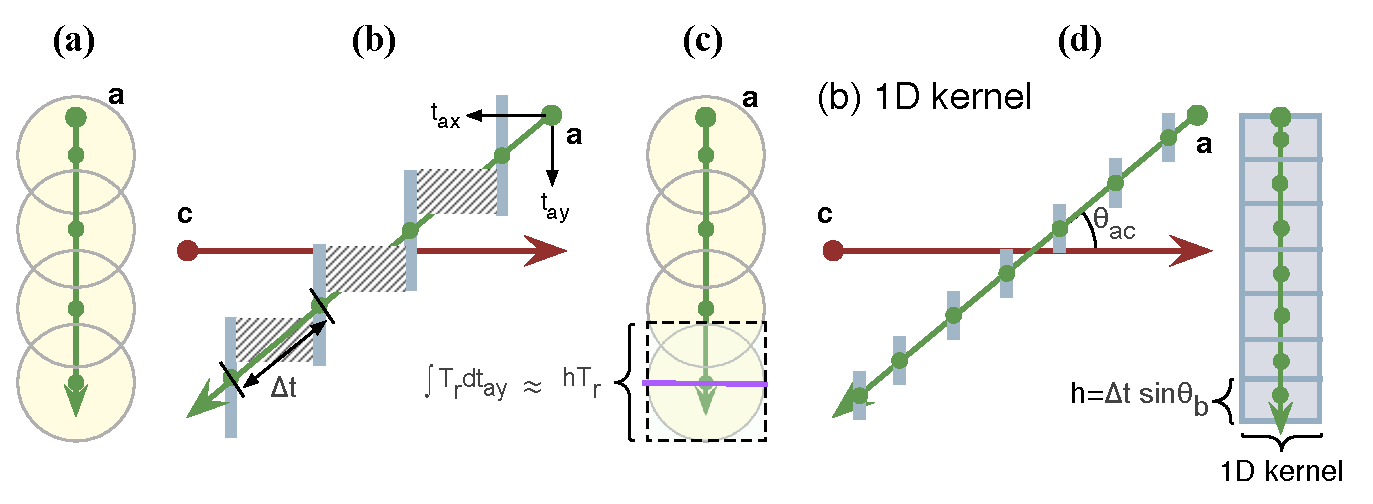
\includegraphics[width=\thewidth]{figures/pm/bb1d}
	\caption{由于2D核函数垂直于查询光束,因此它在光子光束上的步进分别是垂直和平行于查询光束方向上两个步进的结果,而在垂直于查询光线方向上的步进则会产生重叠;这里使用对核函数降维的方法来消除重叠区域的积分计算}
	\label{f:pm-bb1d}
\end{fullwidth}
\end{figure}

为了消除该积分,这里可以采用前面提到的核函数降维的方法(见图\ref{f:pm-averaging-transmittance}),首先将该圆形的2D核函数表述为沿查询光束视角\footnote{因为我们的目标是要降维,所以必须首先确定在哪一维度上进行模糊。}的2D矩形核函数,如图\ref{f:pm-bb1d}(c)所示。对于重叠区域(即是积分范围),它们来自于光照光束上一个步进尺寸$\Delta$在图\ref{f:pm-bb1d}(c)上的投影,所以这里平均透射比需要平均的长度为$\Delta t\sin{\theta_a}$。所以最后我们可以得到降维的估计为(如图\ref{f:pm-bb1d}(d)所示):

\begin{equation}\label{e:pm-bb1d}
	\langle I\rangle_{B-B1D}=T_r(t_a) \rho(\tilde{\mathbf{b}},\mathbf{b}) \cfrac{K_1(\tilde{\mathbf{b}},\mathbf{b})}{\sin{\theta_{ac}}}T_r(t_c)
\end{equation}

上述保证了1D核函数之间无论从什么角度看都不会重叠,实际上1D核函数在光子光束上步进形成的面,与查询光束的角度正好为$\theta_{ac}$,,你可以想象图\ref{f:pm-bb1d}(d)中的穿过绿色光子光束并垂直于纸面的平面,1D核函数和光子光束和查询光束都是垂直的,如图\ref{f:pm-estimators}(i)所示。




\paragraph{数据结构}
虽然光子光束的查询需求和上一节是相似的,但是沿着另一条光束多个离散点的连续查询却使得BVH会非常低效,我们将看到\cite{a:UnifyingPointsBeamsandPathsinVolumetricLightTransportSimulation}直接使用一个索引表格的数据结构来进行光束与光束之间的相交查询。






\subsection{异质介质中的透射比估计}
从上节的内容我们看到,参与介质中光照传输的问题最后都可以归结为透射比(transmittance)\myindex{透射比}{transmittance}的计算,也可以称作部分可见性(fractional visibility)它表示光子沿直线传输一定距离$d$之后存活下来的光子的比率,用于计算在介质存在的情况下,光照在两点之间的传输:

\begin{equation}
	T(d)= \cfrac{L_o}{l_i}=\exp{\Bigg(-{\rm \int}^{d}_0}\mu(x){\rm d}x\Bigg)
\end{equation}

这里$L_i$表示传输起点的辐射能量,$L_o$表示到达距离$d$处剩余的能量。在同质介质中,消光系数$\mu$是一个与空间位置无关的常数,上式就是一个简单的指数计算:$T(d)=\exp(-d\mu)$;然而在异质介质中,由于消光系数在每个位置处的值可能都是不同的,透射比的计算需要对整个$d$的长度进行积分,计算非常复杂,如图\ref{f:pm-transmittance-vs-fps}(a)展示了透射比和相关系数之间的关系。

\begin{figure}
	\sidecaption
	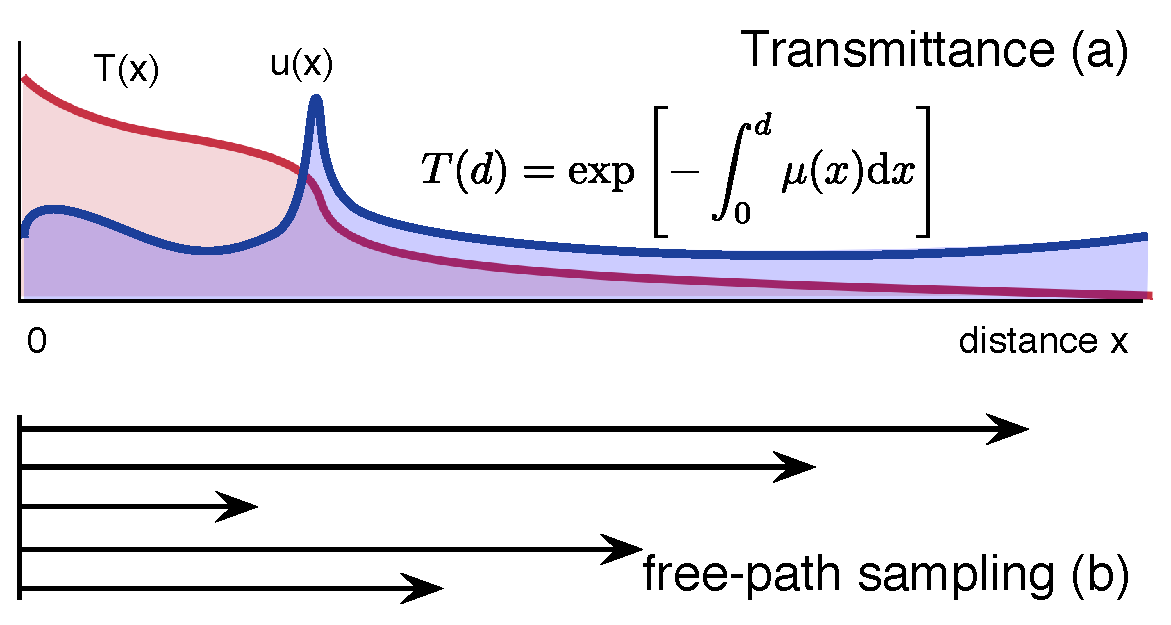
\includegraphics[width=0.65\textwidth]{figures/pm/transmittance-1}
	\caption{透射比计算和自由路径采样是参与介质渲染中的两大基础问题,(a)透射比描述了一束光子在给定距离的传输后剩余下来的能量,而(b)自由路径采样则尝试计算一个光子能够在介质中自由传播的距离}
	\label{f:pm-transmittance-vs-fps}
\end{figure}

参与介质渲染的另一个非常基础的问题为:计算一个光子在介质中能够无障碍传播的距离,也即是光子在第一次与介质中的粒子发生交互(吸收或散射)之前自由传播的距离,这即是前面提到的自由路径采样(free-path sampling)\myindex{自由路径采样}{free-path sampling},它可以用来比如生成光子光束分布图,如图\ref{f:pm-points-vs-beams}(b)所示。

自由路径采样和透射比的计算是非常相关的两个问题,本节我们就将介绍一些常见的自由路径采样方法,并介绍怎样借助自由路径采样的方法来对透射比进行估计,我们将看到它们两者之间的联系,以及这些方法怎样被运用于工业中。




\subsubsection{自由路径采样}
光子在介质中的传播受粒子的吸收和散射行为的影响,前面已经说明,我们使用概率的方式来描述这种粒子的行为,其中$\mu(x)$表示光子在$x$处发生交互的概率。

由于并无已知的自由路径的概率分布形式,现有方法大多通常获得自由路径的累积分布函数(cumulative distribution function,CDF)\myindex{累积分布函数}{cumulative distribution functio},然后通过逆变换方法(inversion method)\myindex{逆变换方法}{inversion method}对自由路径进行采样。

\begin{figure}
	\sidecaption
	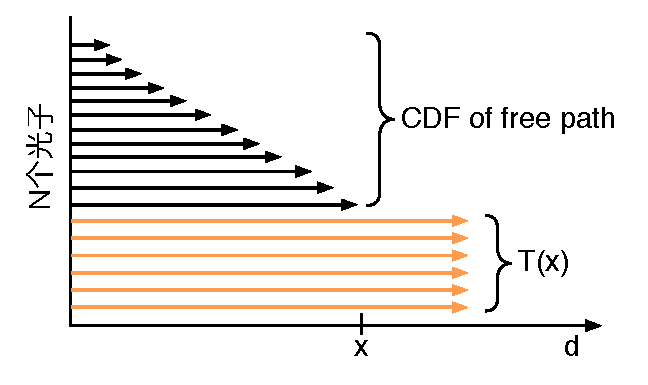
\includegraphics[width=0.5\textwidth]{figures/pm/free-path-cdf}
	\caption{$N$个光子沿直线传播的过程,实际上就是累积光子与各个位置的粒子发生碰撞的概率的过程,$T(x)$反应了$N$个光子经过距离$x$传播后没有与粒子发生碰撞的概率,则$1-T(x)$累积了在距离$x$的传播过程中与每个位置处粒子发生碰撞的概率}
	\label{f:pm-free-path-cdf}
\end{figure}

让我们重新思考透射比$T(d)$意义,透射比表示的是一定数量的光子经过距离为$d$的直线传播后存活下来光子的比例,它不是单个光子的行为,实际上它无法描述单个光子的行为,它描述的是多个光子的行为的和。例如图\ref{f:pm-free-path-cdf}所示,假设有$N$个光子从距离0处出发开始沿某个方向直线传播,在传播过程中的每一个地方都有一定数量的光子与粒子发生碰撞,这实际上就是自由路径的概率分布,当光束传播到距离$x$处时,透射比的值$T(x)$表示存活下来(即没有与粒子发生碰撞)的光子比例,则其他所有与粒子发生碰撞的概率之和构成了自由路径的累积分布函数:

\begin{equation}
	P(s)=1-T(s)=1-\exp(-\tau(0,s))
\end{equation}

由此我们可以通过对一个均匀分布的随机数$r$采样,然后通过求解下述方差来获得该随机数对应的自由路径长度$s$的值:

\begin{equation}\label{e:pm-free-path-random-number}
	r=P(s)\Leftrightarrow -\log(1-r)=\tau(0,s)
\end{equation}

这里$\tau$即是前面介绍的光学深度(optical depth)\myindex{光学深度}{optical depth}。如果介质是同质的,那么上式可以通过分析的方法直接计算而出;然而现实中大部分介质都是异质的,这也是本节要讨论的重点。

如果异质介质能够被划分成多个同质的区域,则每个同质的区域可以使用分析的方法计算出该部分的光学深度,如图\ref{f:pm-tracking}(a)所示,这时每个区域内的消光系数是常数,我们可以通过检查沿光线方向上所有区域的累积光线深度是否大于$-\log(1-r)$来近似求解距离样本$s$的值:

\begin{equation}\label{e:pm-regular-tracking}
	\sum^{n-1}_{i=0}\sigma_{ti}\Delta s\leq-\log(1-r)<\sum^{n}_{i=0}\sigma_{ti}\Delta s
\end{equation}

上述的方法称为常规跟踪(regular tracking)\myindex{常规跟踪}{regular tracking},这里的$n$表示光线传播过程中经过的多个不同消光系数的同质区域。然而要想获得这样的同质区域是非常困难和复杂的,因此它仅适用于比较简单的情形。但是这给了我们一种启发,即如果假设异质介质的局部区域是同质的,那么可以将介质划分为多个间隔相等的区域,使每个区域内可以看做是近似同质的,这就是传统的光线步进(ray marching)\myindex{光线步进}{ray marching}的方法,如图\ref{f:pm-tracking}(b)所示。

很显然,光线步进是有偏的估计方法,因为它可能漏掉很多重要的局部变化的信息。为了减少光线步进的偏差,我们需要使用更小的间隔区域,然而这又增加了式\ref{e:pm-regular-tracking}累积计算成本。

为了消除估计的偏差,我们需要将数值近似方法转向为依靠概率的随机方法,现行大部分随机方法都是基于或者改进的称为增量跟踪的方法,以下我们将具体介绍其原理及其衍生方法。




\subsubsection{增量跟踪}\label{sec:pm-delta-tracking}
严格意义上说,上面讨论的常规跟踪并不完全是一种近似方法,它使用的是第\ref{chp:mc}章讨论的逆变换方法,根据那里的内容,逆变换方法首先对累积分布函数进行均匀分布采样,然后通过求该累积分布函数的反函数来求随机抽样的值,该反函数和欲求的随机变量具有相同的分布。但是这里的反函数并没有解析的方法可以求得,因此常规跟踪在求反函数值的时候使用了近似方法,这也使得原本的随机方法仍然包含了偏差。

当逆变换算法的反函数计算成本较高,或者根本没有显示表达式时,另一种常见的替代方法是取舍算法(acceptance-rejection method)\myindex{取舍算法}{acceptance-rejection method},取舍方法在一个更均匀的空间内产生一个随机数,然后判断该随机数处的值是否满足一定的条件而被接受,否则重复上述过程。在路径的自由采样中,消光系数提供了某个位置被接受或拒绝的条件,剩下的我们还需要构造一定的边界空间就可以使用取舍算法来估计自由路径的长度。

增量跟踪(delta tracking)\myindex{增量跟踪}{delta tracking}就是一种基于取舍方法的用来进行自由路径采样的方法,它又称为伍德科克跟踪(Woodcock tracking)\myindex{伍德科克跟踪}{Woodcock tracking}\cite{a:TechniquesusedintheGEMcodeforMonteCarloneu-tronicscalculationsinreactorsandothersystemsofcomplexgeometry},伪散射(pseudo scattering)\myindex{伪散射}{pseudo scattering},洞穴跟踪(hole tracking)\myindex{空穴跟踪}{hole tracking}或者空位碰撞\footnote{我们将在后面说明这些名字的含义。}(null-collision)\myindex{空位碰撞}{null-collision},它首次被\cite{a:UnbiasedGlobalIlluminationwithParticipatingMedia}引入计算机图形学中用于渲染参与介质。现在已成为介质渲染中透射比计算与自由路径采样的主要基础,例如\cite{a:FreePathSamplinginHighResolutionInhomogeneousParticipatingMedia,a:EfficientFreePathSamplinginInhomogeneousMedia,a:ResidualRatioTrackingforEstimatingAttenuationinParticipatingMedia,a:ProgressivePhotonBeams}等。

\begin{figure}
	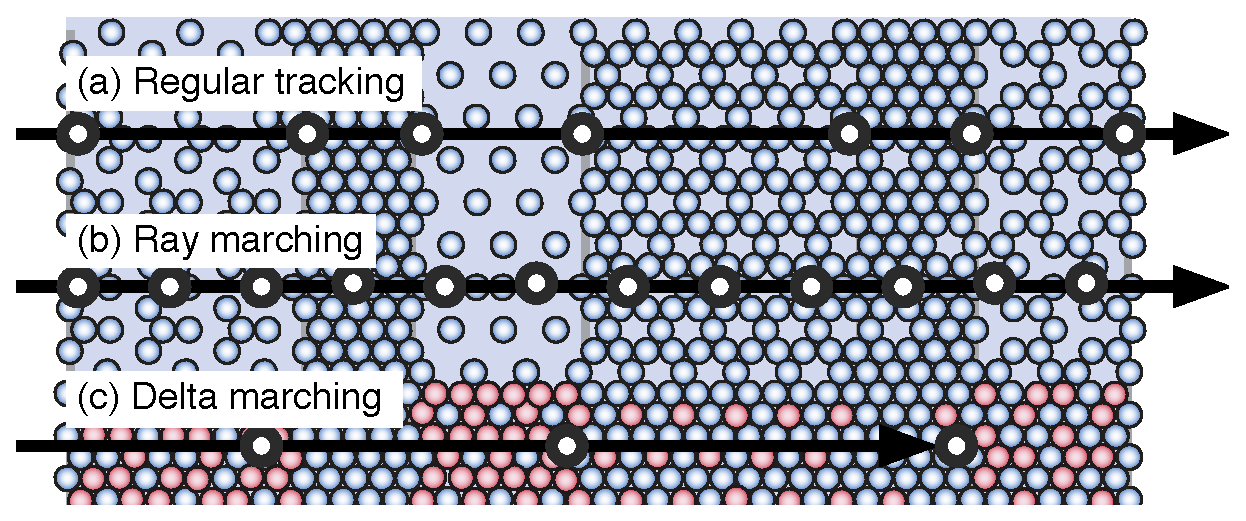
\includegraphics[width=1.0\textwidth]{figures/pm/tracking}
	\caption{常用的用于估计透射比和自由路径采样的几种不同的方法,(a)常规跟踪方法通过寻找介质之间的相交边界来划分多个同质区域,然而对每个同质区域使用分析方法求解,(b)光线步进方法则使用固定的与介质分布无关的间隔,并假设局部间隔区间内是同质的来进行近似计算,(c)增量跟踪则通过使异质介质同质化,然后使用取舍方法来对自由路径进行无偏估计}
	\label{f:pm-tracking}
\end{figure}

回想前面的内容,要想使用取舍方法对某个函数进行采样,我们首先需要使用一个更简单形式的函数“包围住”采样函数,该简单函数通常具有非常简洁的形式使得可以以非常低的计算量对其直接进行采样,例如一个常数函数(如图\ref{f:mc-rejection-idea}所示)或者一个更接近采样函数形状的分段线性函数(如图\ref{f:mc-rejection-generalized}所示),然后使用采样函数的值对每个简单函数的采样值进行取舍判断。

所以为了对每个位置处都具有不同消光系数值的异质介质进行路径采样,增量跟踪首先使用以下方法来生成一个更简单的常数函数:即在异质介质中每个“空位处”加入一些虚拟粒子(virtual particles)\myindex{虚拟粒子}{virtual particles},或称为虚构粒子(fictitious particles)\myindex{虚构粒子}{fictitious particles},使得对于混合后的“同质介质”,其消光系数$\bar{\sigma}(s)=\sigma_t(s)+\sigma_v(s)$为一个常数,这里$\sigma_v(s)$表示虚拟粒子的消光系数,$\sigma_t(s)$表示原介质中的真实粒子的消光系数。由于混合后的介质其相关系数为常数,因此上述的操作也称为使异质介质同质化(homogenize)\myindex{同质化}{homogenize},如图\ref{f:pm-tracking}(c)所示,其组合的消光系数又称为一个强函数(majorant)\footnote{majorant的英文原意为: ”A function, or an element of a set, that dominates others or is greater than all others“。}\myindex{强函数}{majorant},它表示一个大于所有真实粒子消光系数$\sigma_t(s)$的值,例如$\sigma(s)=1$\cite{a:ProgressivePhotonBeams},如图\ref{f:pm-delta-tracking}右边小图所示。

那怎样保证新加入的虚构粒子能够不改变原有异质介质的传输行为呢,这通过一个特殊的设置来实现:即使得虚构粒子的反射率为1,并且其相位函数为沿光线传输方向$\omega$的一个脉冲值$\delta(\omega)$,这就使得虚构粒子并不会改变原有粒子的传输行为,因此这就是光子与虚构粒子的碰撞又称为空位碰撞(null-collision)\myindex{空位碰撞}{null-collision}的原因。

\begin{algorithm}
\begin{lstlisting}[language=C++, mathescape]
float DeltaTracking(o, $\omega$, d) {
	t = 0;
	do {
		$\zeta$ = rand();
		t = t - $ \cfrac{\log(1-\zeta)}{\bar{\mu}}$;
		if (t $\geq$ d) break;
		$\xi$ = rand();
	} while ($\xi$ > $ \cfrac{\sigma(o+t*\omega)}{\bar{\sigma}}$);
	
	return t;
}
\end{lstlisting}
\caption{增量跟踪算法的伪代码,它返回一个光子在介质中从起点$o$开始沿方向$\omega$传播的自由路径长度$t$,其中$d$为介质的边界距离}
\label{a:pm-delta-tracking}
\end{algorithm}


有了以上这些准备工作,现在就可以来描述增量跟踪的思路,如算法\ref{a:pm-delta-tracking}所示,首先我们消光系数为$\bar{\sigma}$的同质介质进行距离采样,由于其消光系数为常数,所以式\ref{e:pm-free-path-random-number}可以简化为\footnote{请注意,由于消光系数本身(如图\ref{f:pm-delta-tracking}右边小图所示)并不能作为自由路径的概率分布函数,所以这里仍然需要使用上节讨论的逆变换算法来将随机数与消光系数产生联系。}(算法\ref{a:pm-delta-tracking}第4行):

\begin{equation}
	-\log(1-r)=\bar{\sigma}\zeta
\end{equation}

然后对于每个自由路径长度$t$,我们使用概率的方法来决定其是否被接受或拒绝,由于每个位置处要么为虚构粒子要么为真实粒子,它们的概率取决于该处的真实消光系数$\sigma_t$,因此我们可以通过产生一个新的随机数$\xi$,并通过比较$\xi>\sigma_t/\bar{\sigma}$来接受或拒绝该采样距离,如算法\ref{a:pm-delta-tracking}第8行。

\begin{figure}
	\includegraphics[width=1.\textwidth]{figures/pm/delta-tracking}
	\caption{增量跟踪借鉴了取舍方法的思路,它首先对异质介质添加一些虚构粒子使其同质化,其同质的消光系数为一个常数$\bar{\sigma}$,然后每一步对$\bar{\sigma}$进行采样,并通过判断采样值对应位置处是否为真实理解来接受或拒绝该采样值}
	\label{f:pm-delta-tracking}
\end{figure}

需要注意的是,我们的目标是要获得一个光子在介质中无障碍传输的距离,换句话说,一个光子一直自由传输直到碰到一个真实粒子。所以,当一个距离被拒绝之后,它表明当前距离处的粒子为虚构粒子,所以光子会以该处为起点继续传播,因此我们需要累加每个采样的距离值,如算法\ref{a:pm-delta-tracking}第5行所示,这是增量跟踪算法不同于传统取舍算法的地方。其原因其实是因为$\sigma(x)$并不直接是这里要采样的函数(即自由路径)的概率密度,实际上由于消光系数是持续作用的,累加的路径长度才正好对应以消光系数为概率密度函数。

同取舍方法一样,增量跟踪方法的缺点是,当介质的平均消光系数大大小于使用的最大消光系数$\bar{\sigma}$时(即添加的虚拟粒子越多的时候),其计算成本大大增加,这是因为随机数$\xi$光子更容易停留在虚拟粒子上使得路径$t$被接受的概率大大降低,需要使用更多的样本,估计的方差也会增大。

\cite{a:FreePathSamplinginHighResolutionInhomogeneousParticipatingMedia}通过对介质计算分段的组合消光系数值$\bar{\omega}$来解决上述问题,如图\ref{f:pm-super-voxels}所示,介质首先被均分成一个低分辨率的超体素(super voxel)\myindex{超体素}{super voxel}的结构(超体素的尺寸通常要远大于使用光线步进方法需要的步进尺寸),每个超体素的网格存储这该区域内的一个最大消光系数值$\sigma_{\max}$,算法首先以$\bar{\sigma}=1$的同质介质生成一个距离随机数,然后搜索超体素网格查询与该长度的光线相交的网格及其网格内的位置,并使用三线性插值算法计算处该位置处的最大消光系数$\sigma_{\max}(s)$然后以此对建议长度进行取舍。

\begin{figure}
	\sidecaption
	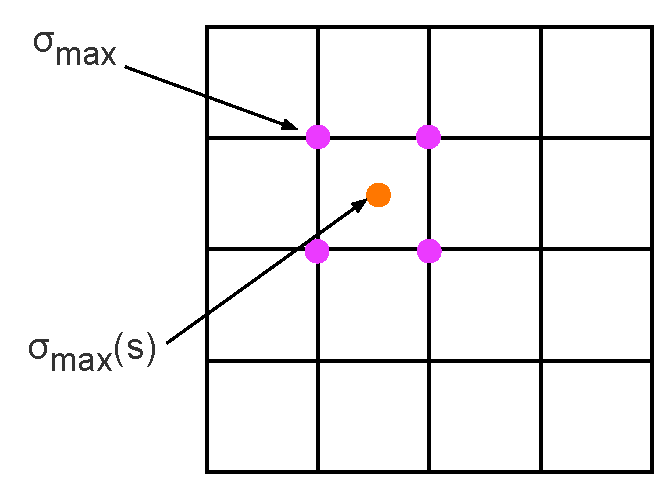
\includegraphics[width=0.5\textwidth]{figures/pm/super-voxels}
	\caption{超体素网格存储着最大消光系数值$\sigma_{\max}$,它可以用多项式插值的方法计算出网格内每个位置处的最大消光系数$\sigma_{\max}(s)$的值}
	\label{f:pm-super-voxels}
\end{figure}





\subsubsection{透射比估计}
同样,我们没有透射比的概率密度函数,所以不能直接通过一般直接采用的随机方法得出。透射比是一个由消光系数导致的交互行为(吸收或散射)累积的结果,因此传统的光线步进(ray marching)\myindex{光线步进}{ray marching}可以用于近似透射比的计算,如\cite{a:AComprehensiveTheoryofVolumetricRadianceEstimationusingPhotonPointsandBeams}中实现的那样,首先将光束的长度划分成多个等间隔的片段,并假设每个局部间隔内的消光系数近似为一个常数,然后可以通过类似式\ref{e:pm-regular-tracking}的方式对式\ref{e:pm-transmittance}执行累加以得出指定长度的透射比的值。

很显然,光线步进的方法是有偏的。为了获得一个无偏的估计,重新考虑如图\ref{f:pm-free-path-cdf}所示的透射比和自由路径的关系,对于$N$个光子在场景中传播,所有传播路径大于$x$的光子的比例就可以作为$T_r(x)$的估计。

基于此观察,一种基于自由路径采样来对透射比进行估计的方法被提出。假设一个给定的自由路径采样方法,例如前面讨论的增量跟踪及其改进方法,$d(\mathbf{x},\vec{\omega})$,它对于一个给定的起始点$x$及光线传输方向$\vec{\omega}$返回一个距离采样值,则距离$s$处的透射比可以通过数那些距离$\geq s$的路径的比例来进行估计:

\begin{equation}
	T_r(\mathbf{x},\vec{\omega},s)=E\Bigg[ \cfrac{1}{n}\sum^{n}_{j=0}H(d(\mathbf{x},\vec{\omega})-s)\Bigg]
\end{equation}

这里$H$是一个海维赛阶梯函数(Heaviside step function)\myindex{海维赛阶梯函数}{Heaviside step function},或称为单位阶梯函数(unit step function)\myindex{单位阶梯函数}{unit step function},对于$n\geq 0$,$H[n]=1$,否则$H[n]=0$。上述方法又称为平均自由路径采样(mean free path sampling)\myindex{平均自由路径采样}{mean free path sampling}法,它被运用于\cite{a:ProgressivePhotonBeams,a:FreePathSamplinginHighResolutionInhomogeneousParticipatingMedia}等。

上述方法的缺点是,每个自由路径采样对透射比的贡献是一个二元的值:当路径长度超过$s$时为1,否则为0,因此透射比的估计包含很大的方差;此外,和传统的增量跟踪一样,上述方法的缺点是当介质中的虚拟粒子数量很多的时候,由于自由路径会更多地与虚拟粒子发生碰撞,导致计算量增加,图\ref{f:pm-delta-vs-ratio}(a)和(b)显式了单个相同长度的自由路径在不同密度介质中与虚拟粒子发生碰撞的次数(垂直方向的虚线)。

\begin{figure}
\begin{fullwidth}
	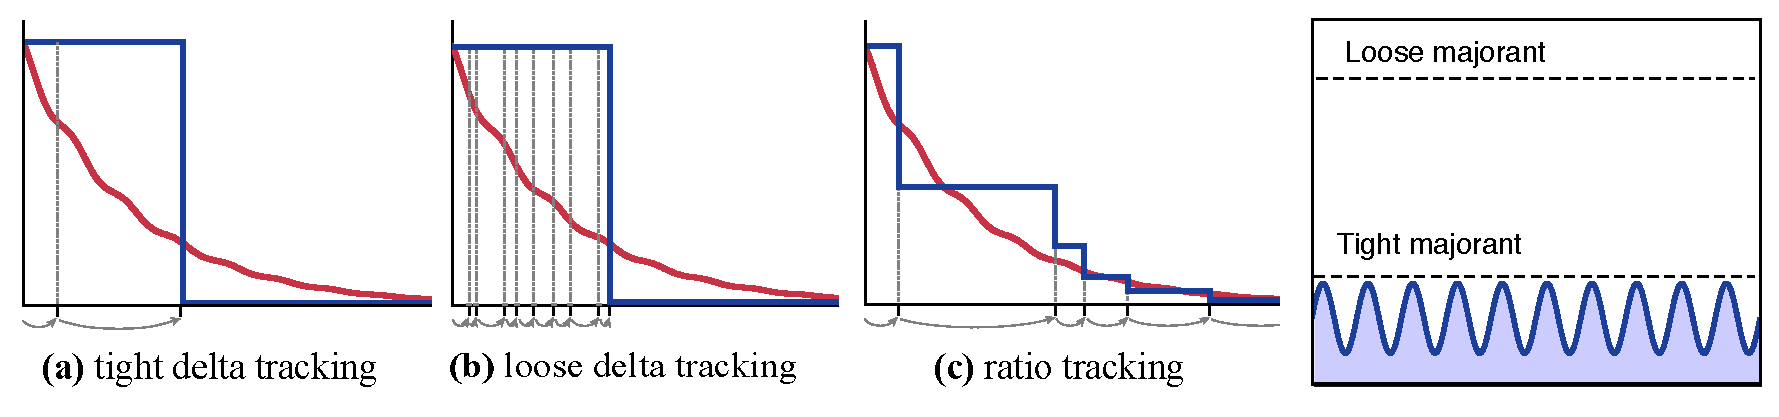
\includegraphics[width=\thewidth]{figures/pm/delta-vs-ratio}
	\caption{传统基于增量跟踪的透射比估计方法具有较大的方差(对比(a)和(c)),并且当介质中虚拟粒子较多时,每个自由路径的计算量大大增加(b)}
	\label{f:pm-delta-vs-ratio}
\end{fullwidth}
\end{figure}




\paragraph{比例跟踪}
在增量跟踪算法中,一条自由路径的传输总是按照每个距离处的真实粒子的比例来概率性地决定其是否需要继续传输或被终止,因此每个路径采样对透射比的贡献要么是0(被终止),要么是1(继续传输)。

上述过程可以看做是一个基于俄罗斯轮盘的随机行走的过程,只不过其使用的终止概率为0或1;与此相反,我们可以将终止概率设置为局部真实光子的比例,即消光系数。在蒙特卡洛模拟中,俄罗斯轮盘经常被用来作为对贡献值进行加权的方法\cite{a:ComparativeanalysisofdiscreteandcontinuousabsorptionweightingestimatorsusedinMonteCarlosimulationsofradiativetransportinturbidmedia}:与其概率性地终止一个事件,我们让它继续随机行走直到达到指定的边界条件,并对其贡献值使用分配一个权重系数。

\cite{a:ResidualRatioTrackingforEstimatingAttenuationinParticipatingMedia}基于此提出了比例跟踪(ratio tracking)\myindex{比例跟踪}{ratio tracking}的方法,在每一步距离采样中,它对路径分配一个与该出虚拟粒子比例相等的权重系数,并使每条路径持续随机行走知道满足超出指定的传输长度,最终每条路径的贡献值被所有与虚拟粒子发生碰撞的联合概率加权:

\begin{equation}\label{e:pm-ratio}
	\langle T(d)\rangle_R=\prod^{K}_{i=1}\Bigg(1- \cfrac{\sigma(x_i)}{\bar{\sigma}}\Bigg)
\end{equation}

这里被乘数表示每个碰撞发生的位置$x_i$处虚拟粒子相对于所有粒子的比例,这可以通过该位置处的消光系数计算而出。

\begin{algorithm}
\begin{lstlisting}[language=C++, mathescape]
float RatioTrackingEstimator(o, $\omega$, d) {
	t = 0;
	T = 1;
	do {
		$\zeta$ = rand();
		t = t - $ \cfrac{\log(1-\zeta)}{\bar{\mu}}$;
		if (t $\geq$ d) break;
		T = T * (1 - $ \cfrac{\sigma(o+t*\omega)}{\bar{\sigma}}$);   //联合概率权重系数
	} while (ture);
	
	return T;
}
\end{lstlisting}
\caption{使用比例跟踪算法用于估计透射比的伪代码,它返回一个光子在介质中从起点$o$开始沿方向$\omega$传播距离为$d$的透射比}
\label{a:pm-ratio-tracking}
\end{algorithm}

算法\ref{a:pm-ratio-tracking}显式了比例跟踪估计的伪代码,图\ref{f:pm-delta-vs-ratio}(c)显式了一条路径下各个碰撞点处贡献值随路径长度的变化。比例跟踪的优点是它很好地利用了在路径跟踪过程中的信息,而不是简单地使用一个二元的判断。比例跟踪提供了一个分段常数来近似透射比函数,相比增量跟踪,它与真实的透射比曲线的形状更加接近。

相较于增量跟踪,比例跟踪唯一的缺点是对于每条路径,它需要多一些额外的路径采样计算,这在一些情况下会比增量跟踪要低效,但是大多数情况下比例跟踪的结果都要好得多。例如当联合消光系数对介质的包围较为松散(即虚拟粒子的数量较多)时,如图\ref{f:pm-delta-tracking}右边小图所示,这需要更多的路径跟踪步骤,比例跟踪能够以更好的分段常数函数来近似真实透射比的分布,如图\ref{f:pm-delta-vs-ratio}(c)所示;当联合消光系数对介质的包围较为密集时,比例跟踪的优势就逐步下降,在极端的$\bar{\sigma}=\sigma_t$的情况下,光子不与任何虚拟粒子发生交互,此时两者呈现一样的结果。

所以从中可以看出,比例跟踪在虚拟粒子越多的情况下,对估计结果的帮助更大,反之越小。接下来我们将介绍一种改进的方法用于在虚拟粒子数量较少的情况下改善比例跟踪的效率。




\paragraph{残留跟踪}
当组合消光系数$\bar{\sigma}$的值比较大时,此时介质具有较多的虚拟粒子,光子更容易与虚拟粒子发生碰撞,因此上面讨论的比例跟踪需要经历更多的尝试才能达到终止条件。\cite{a:ResidualRatioTrackingforEstimatingAttenuationinParticipatingMedia}进一步提出了一种称为残留跟踪的方法用于降低组合消光系数的值,以提高比例跟踪(或者甚至某些条件下)增量跟踪的计算效率。

残留跟踪(residual tracking)\myindex{残留跟踪}{residual tracking}借鉴了分离变量的思路,首先一个控制消光系数(control extinction coefficient)\myindex{控制消光系数}{control extinction coefficient}$\sigma_c(x)$被引入介质中,控制消光系数是一个简单的可以以分析的方法就光线深度的消光系数,此时新的透射比公式变为:

\begin{equation}\label{e:pm-residual}
\begin{aligned}
	T(d)&=\exp\Bigg(-{\rm \int}^{d}_0\sigma(x){\rm d}x\Bigg)\\
	&=\exp\Bigg(-{\rm \int}^{d}_0\sigma_c(x)+\sigma(x)-\sigma_c(x){\rm d}x\Bigg)\\	
	&=\underbrace{\exp(-\tau_c(d))}_{\text{Control transmittance}}\underbrace{\exp\Bigg(-{\rm \int}^{d}_0\sigma(x)-\sigma_c(x){\rm d}x\Bigg)}_{\text{Residual transmittance}}
\end{aligned}
\end{equation}

上式的第一个指数项称为控制透射比(control transmittance)\myindex{控制透射比}{control transmittance},它使用控制消光系数计算而得,它可以看做是$T(d)$的一个粗略近似;第二项表示控制透射比和实际透射比之间的一个差值,称为残留透射比(residual transmittance)\myindex{残留透射比}{residual transmittance}$T_r$,对应的残留消光系数为:$\sigma_r(x)=\sigma(x)-\sigma_c(x)$,可以看出,在某些情况下残留消光系数的值可能是负数。

\begin{figure}
	\includegraphics[width=1.0\textwidth]{figures/pm/residual}
	\caption{残留跟踪采用了控制变量的思路,它将消光系数(a)分割为控制消光系数(b)和残留消光系数(c),最终实际的透射比为控制透射比和残留透射比的乘积,前者通过分析的方法计算而出,而后者是以如比例跟踪或增量跟踪等方法计算}
	\label{f:pm-residual}
\end{figure}

图\ref{f:pm-residual}显式了残留跟踪将消光系数分离为控制消光系数和残留消光系数的概念,残留透射比可以使用上述的增量跟踪进行估计,而控制透射比可以用任何可以以简单分析方法计算,例如常数控制消光系数。

值得注意的是,由于透射比是指数形式的积分,所以即使是一个常数的控制变量,如果它减少了残留指数积分项的变化率,则也能够减少估计的方差。可以看到,残留跟踪将比例跟踪的分段常数转变为了分段指数的形式。

通过简单地将式\ref{e:pm-ratio}中的消光系数调整为残留消光系数,我们得到一个残留比例跟踪(residual ratio tracking)\myindex{残留比例跟踪}{residual ratio tracking}估计:

\begin{equation}
	\langle T_r(d)\rangle_{RR}=\prod^{K}_{i=1}\bigg(1- \cfrac{\sigma_r(x_i)}{\bar{\sigma}_r}\bigg)=\prod^{K}_{i=1}\bigg(1- \cfrac{\sigma(x_i)-\sigma_c}{\bar{\sigma}_r}\bigg)
\end{equation}

由于残留消光系数可能是负的,如图\ref{f:pm-residual}(c)所示,这意味着光子的能量反而会增加(负的吸收相当于正的增加),因此这种情况下使用增量跟踪是不合适的,因为它无法正确处理这种情况;而在比例跟踪中,对每条路径被记录一个权重系数,这意味着权重系数可能大于1而已,可以很容易地处理这种情况。

对于控制消光系数,一般可以简单地选择原始消光系数的最小,最大或者平均值,通常平均值具有更好的结果(更小的方差)。需要注意的是,平均消光系数是针对一条光线上的平均消光系数,所以它需要对每条单向单独计算,这增加了计算成本,\cite{a:ResidualRatioTrackingforEstimatingAttenuationinParticipatingMedia}使用了\cite{a:FreePathSamplinginHighResolutionInhomogeneousParticipatingMedia}中的超体素的概念,分别对一个较大范围的空间计算一个平均值来加上平均消光系数的计算。

残留比例跟踪已经被运用于Disney的Hyperion渲染器\cite{a:ResidualRatioTrackingforEstimatingAttenuationinParticipatingMedia}以及《超能陆战队》\cite{a:BigHero6:IntothePortal}及其后续电影产品中。

\cite{a:UnbiasedLightTransportEstimatorsforInhomogeneousParticipatingMedia}进一步将残留跟踪及其控制变量的思路扩展到整个介质微观的粒子交互模型,在这种模型中,介质的密度不仅可以被增加(虚拟粒子)以维持一个常数的消光系数(同质介质)用来进行直接路径采样,同时它还可以被减少(移除真实粒子),在这种模型下残留跟踪成为一种特殊情况,并且该模型可以用于计算粒子的散射行为,而不仅仅是透射比的计算。





\subsection{统一光子,光束和路径估计}\label{sec:pm-upbp}
到目前为止,我们已经介绍了很多不同的参与介质采样技术,例如传统的双向路径追踪,基于光子和光束的辐射亮度估计以及光束辐射亮度估计,不同的采样技术都具有不同的方差,偏差(对于辐射亮度估计)及收敛速度,也有着自己独特的对目标函数某些重要部分的采样能力,虽然每种采样技术理论上都可以收敛到正确的结果,但是我们希望估计具有最小的方差以及最快的收敛速度,使用复合重要性采样将这些不同的采样技术组合起来是我们本节要讨论的内容。

为了对进行复合重要性采样的必要性提供依据,\cite{a:UnifyingPointsBeamsandPathsinVolumetricLightTransportSimulation}对上述各种不同采样技术的方差进行了分析,其展示了不同采样技术在不同几何配置下的相对性能,例如不同的核估计带宽以及不同的平均自由路径长度都会对估计有不同的影响,从其结果可以看出,没有任何一个采样技术能够在所有条件下优于其他采样技术。我们这里不会方差分析的过程进行讨论,而是直接介绍怎样使用复合重要性采样将它们组合起来,这里很多概念和原理与前面介绍的顶点连接与合并是类似的,但是这里多了一些针对光束的一些新的概念,因此涉及的内容要相对复杂一些。




\subsubsection{扩展空间}
我们在前面顶点连接与合并(第\ref{sec:pm-vcm}节)一节讨论了双向路径追踪和光子映射两种采样技术的复合,在那里我们对贡献函数乘以一个表示光子估计的核估计函数,然后使得使用光子映射的路径保留在了常规路径空间当中,因此可以和双向路径追踪采样技术进行重要性复合。本节,我们将进一步推导出一个更一般的扩展空间的估计公式,使得任意维度的估计式都可以在一个共同的空间进行复合。

复合重要性采样(multiple importance sampling)\myindex{复合重要性采样}{multiple importance samplin}必须发生于同一空间,由于函数定义域空间的各个维度是相互独立的,所以如果我们将那些“额外的”维度投射到低纬度,并不会影响抽样在低纬度中的分布。借助这样的思路,为了使不同维度的采样可以在同一空间进行复合,我们定义一个扩展空间(extended space)\myindex{扩展空间}{extended space},根据蒙特卡洛方法,扩展空间的积分:

\begin{equation}
	I^{E}_i={\rm \int}_{\mathcal{D}_x}{\rm \int}_{\mathcal{D}_{yi}}f(x,y_i){\rm d}y_i{\rm d}x	
\end{equation}

\noindent 可以使用以下公式进行估计:

\begin{equation}
	\langle I^{E}_i\rangle= \cfrac{1}{m}\sum^{m}_{j=1} \cfrac{f(X_j,Y_{i,j})}{p(X_j,Y_{i,j})}
\end{equation}

\noindent 在这里,假设围绕$\mathcal{D}_{yi}$空间的积分被看做使用不同核函数进行模糊,则随机变量$Y_{i,j}$对应于光子或者光束,因此上式可以看做是$I$的一个有偏估计,其中$I$为$\mathcal{D}_x$空间的积分。为此我们的目标便是将一些在扩展空间具有不同的形式估计$I^{E}_i$,在常规空间进行组合,并使其方差最小。

假设我们有$u>0$种常规空间的采样技术$p_1(x,\cdots,p_u(x)$,以及$n-u>0$中扩展空间的采样技术$p_{u+1}(x,y_{u+1}),\cdots,p_n(x,y_n)$,其中每种扩展空间的采样技术都可能具有不同的维度,我们定义一个扩展组合估计(extended combined estimator)\myindex{扩展组合估计}{extended combined estimator}$F^{C}$为:

\begin{equation}\label{e:pm-extended-combined-estimator}
	F^{C}=\sum^{n}_{i=1} \cfrac{1}{n_i}\sum^{n_i}_{j=1}F^{C}_{i,j}
\end{equation}

\noindent 其中,随机变量$F^{C}_{i,j}$定义为:

\begin{equation}
	F^{C}_{i,j}=\begin{cases}
		F_{i,j} & \text{ if } 1\leq i\leq u\\
		F^{E}_{i,j}& \text{ if } u< i\leq n
	\end{cases}
\end{equation}

\noindent $F_{i,j}$和$F^{E}_{i,j}$分表表示常规空间和扩展空间的贡献函数,定义为:

\begin{equation}
	\begin{aligned}
		F_{i,j}&=w_i(X_{i,j}) \cfrac{f(X_{i,j})}{p_i(X_{i,j})}\\
		F^{E}_{i,j}&=w_i(X_{i,j}) \cfrac{f_i(X_{i,j},Y_{i.j})}{p_i(X_{i,j},Y_{i,j})}
	\end{aligned}
\end{equation}

式\ref{e:pm-extended-combined-estimator}组合了$u$种常规空间的采样技术,以及$n-u$种扩展空间的采样技术。值得注意的是,在常规空间,$f_i(x)$的形式都是相同的,只是使用的采样技术$p_i(x)$不同,然而在扩展空间中,$f_i(x,y)$的形式往往是不同的,比如我们可以使用不同的核函数,或者不同的拥有不同偏差的其他模型。此外,对最终贡献值的权重计算只在常规空间发生,因为我们要从常规空间去看待这个贡献值,并进行加权,以下我们介绍上式中使用的权重系数的计算。




\subsubsection{扩展平衡启发式}
在蒙特卡洛估计中,每种采样技术可以拥有不同空间贡献值计算$ \cfrac{f(x)}{p(x)}$,但是要对不同的采样技术进行复合,则需要在一个共同的空间下去分配各自的权重系数。与\cite{a:RobustMonteCarloMethodsforLightTransportSimulation}的原理类似,\cite{a:UnifyingPointsBeamsandPathsinVolumetricLightTransportSimulation}提出了一个扩展平衡启发式(extended balance heuristic)\myindex{扩展平衡启发式}{extended balance heuristic}:

\begin{equation}
	w_i(x)= \cfrac{n_i/k_i(x)}{\sum^{n}_{k=1}n_k/k_k(x)}
\end{equation}

\noindent 其中:

\begin{equation}
	k_i(x)=\begin{cases}
		\mathlarger{ \cfrac{f^{2}(x)}{p_i(x)}} & \text{ if } 1\leq i\leq u\\
		\mathlarger{{\rm \int}_{D_{yi}} \cfrac{f^{2}_i(x,y_i)}{p_i(x,y_i)}{\rm d}y_i} & \text{ if } u<i\leq n
	\end{cases}
\end{equation}

由于不同的采样技术在$D_{yi}$空间的积分可能具有不同的维度,例如使用不同维度的核函数,因此上述的$k_i(x)$具有不同的形式。可以通过蒙特卡洛方法对上述积分进行估计,即对随机变量$Y_{i,j}$进行采样,然而需要注意的是,对于我们这里使用光子映射的特定场景,由于核函数范围内的光子可能包含了不同长度的路径,因此我们不能对全部核函数包围的空间进行积分,只能对具有相同光源子路径长度的路径进行积分,因为不同长度的光源子路径与摄像机子路径的组合被看成是不同的采样技术(参见前面第\ref{sec:pm-vcm}一节的内容)。实际上,我们在前面的基于点和光束的估计形式(式\ref{e:pm-pp3d}到\ref{e:pm-bb1d})都是针对单个光子或单条光束的,因此在这里上述积分实际上只有一个样本值,那就是在这些估计中用于进行核估计的光子或光束。

虽然对于单个光子点,上述积分计算非常简单,但是对于光束的情况,则仍然需要执行积分计算,这是一个成本比较高的计算,我们将在后面讨论各种采样技术的贡献值及概率密度函数之后,推导出一个近似计算。





\subsubsection{将估计表示为采样技术}
有了对不同维度空间(扩展空间)的估计在其指定共同空间(常规空间)进行复合的理论基础,我们就可以来具体分析前面的各种估计怎样被表述为一种采样技术,这些内容包含定义常规空间$x$,计算每个采样技术的贡献值$f(x)$或$f_i(x,y_i)$,及其概率密度函数$p_i(x)$或$p_i(x,y_i)$,以及明确每个采样技术对应的核估计空间$y_i$。

我们定义常规空间变量$x$为一条全路径$\bar{x}$,由于传统无偏的路径采样技术(例如单,双向路径采样)已经被定义于此空间(其贡献值为$f(x)/p_i(x)$),因此这里仅需要对体积内的估计进行适当的表述。这里仅以三种(即P-P3D,P-B2D以及B-B1D)常见比较简单的估计进行分析,其他的估计可以按此进行分析。


遵循图\ref{f:pm-estimators}(a)中的几何配置,顶点$\mathbf{a}$和$\mathbf{c}$分别位于光源子路径和摄像机子路径的末端,因此全路径$x$可以表述为$\bar{x}=\mathbf{x}_0\cdots\mathbf{a}\mathbf{b}\mathbf{c}\cdots\mathbf{x}_k$。为了使分析更简洁,这里略去所有估计中共同的路径部分,所以定义$x\equiv \mathbf{b}$,$y_i$则分别对应于各个估计的核函数部分,如图\ref{f:pm-y}所示。

使用图\ref{f:pm-estimators}(a)所示的几何配置:给定两个顶点$\mathbf{a}$和$\mathbf{c}$分别位于光源和摄像机子路径的末端,所以全路径为$\mathbf{x}_0\cdots\mathbf{a}\mathbf{b}\mathbf{c}\cdots\mathbf{x}_k$




\paragraph{概率密度函数}
正如前面的内容所述,实际上在不同维度空间进行复合并不影响其概率密度和估计的形式,也就是单个采样技术是不受影响的,只有权重系数的计算是最重要的。但是这里还是稍微分析一下概率密度函数和贡献值函数,可以帮助理解在这些估计中的那些维度是常规空间,那些维度是核函数空间。

\begin{figure}
	\includegraphics[width=1.\textwidth]{figures/pm/y}
	\caption{不同估计中核函数定义域$y$的定义;注意,这里$y$在(a)和(b)中实际上只有一个样本值,只有在$(c)$中才需要进行积分计算}
	\label{f:pm-y}
\end{figure}

首先对于P-P3D估计,如式\ref{e:pm-pp3d}所示,核估计空间为$y_{P-P3D}\equiv \tilde{\mathbf{b}}$,即是3D的光子位置,如图\ref{f:pm-y}(a)所示,其联合概率密度函数为:

\begin{equation}
	p_{P-P3D}(x,y)=p(\mathbf{b},\tilde{\mathbf{b}})=p(\mathbf{b})p(\tilde{\mathbf{b}})
\end{equation}

因为$\mathbf{b}$和$\tilde{\mathbf{b}}$是相互独立的,同样需要注意的是,由于估计式\ref{e:pm-pp3d}已经转换为针对单个光子的形式\footnote{前面已经说明这是为了保证相同的路径长度,因为不同的路径长度组合被视为不同的采样技术。},这里在$y$空间上其实只有一个样本值。

对于P-B2D估计,如式\ref{e:pm-pb2d}所示,首先我们需要对查询光束进行采样,即$p(\omega_c)$,然后需要对$\tilde{\mathbf{b}}$采样使其位于$\mathbf{b}$所在的核估计范围内,这里可以将$\tilde{\mathbf{b}}$的位置表述为与查询光束对齐的坐标系$\vec{t},\vec{u},\vec{v}$中,由于$\vec{t}=\omega_c$已知,因此光子位置仅剩下两个维度,所以这里定义核估计空间为$y_{P-B2D}\equiv (\tilde{u},\tilde{v})$,如图\ref{f:pm-y}(b)所示。其联合概率密度函数为:

\begin{equation}
	p_{P-B2D}=p(\tilde{\mathbf{b}})G(\mathbf{b},\mathbf{c})p(\omega_c)
\end{equation}

同样是因为$\mathbf{b}$和$\tilde{\mathbf{b}}$是相互独立的,但是在这里$\tilde{\mathbf{b}}$的其中一个维度$\vec{t}$已经固定,所以仅剩下两个维度;同样,由于估计式\ref{e:pm-pb2d}已经转换为针对单个光子的形式,这里在$y$空间上其实只有一个样本值。

最后对于B-B1D估计,如式\ref{e:pm-bb1d}所示,核估计空间为$y\equiv \tilde{d}$,如图\ref{f:pm-y}(c)所示,它表示两条光束之间的距离。其联合概率密度函数可表述为:

\begin{equation}
	p_{B-B1D}=p(\omega_a)G(\mathbf{a},\tilde{\mathbf{b}})\sin \theta_{ac}G(\mathbf{b},\mathbf{c})p(\omega_c)
\end{equation}

其中,$\sin\theta_{ac}$来自于B-B2D估计的核函数降维过程中核函数与两条光束之间去重叠的结果,见第\ref{sec:pm-beam-based-estimator}节的内容。这里的核函数空间只有一个维度(即距离$\tilde{d}$),是因为1D的核函数在光子光束上步进形成的面与查询光束平行,并且1D核函数同时垂直于查询光束和光子光束,同样见第\ref{sec:pm-beam-based-estimator}节的内容。




\paragraph{贡献值函数}
给定式\ref{e:pm-pp3d}-\ref{e:pm-bb1d}中的估计形式,以及上述的概率密度函数,运用估计的关系$\langle I\rangle_i=f_i(x,y_i)/p_i(x,y_i)$可以推导出贡献函数$f_i$的形式为:$f_i(x,y_i)=h(x,y_i)K_i(x,y_i)$,其中$K_i(x,y_i)$表示3D,2D或1D的核函数,以及:

\begin{equation}
	h_i(x,y_i)=\rho(\mathbf{a})T_r(\mathbf{a},\tilde{\mathbf{b}})G(\mathbf{a},\tilde{\mathbf{b}})\rho(\tilde{\mathbf{b}},\mathbf{b})G(\mathbf{b},\mathbf{C})T_r(\mathbf{b},\mathbf{C})\rho(\mathbf{c})
\end{equation}





\subsubsection{采样技术/路径分析}
根据上述的分析,给定长度为$k$的路径,$k-1$个散射顶点,其中如果$m$个顶点处于介质中,则上述的三种估计将为路径采样增加3$m$种采样技术,如图\ref{f:pm-beam-gathering}所示,当然\cite{a:UnifyingPointsBeamsandPathsinVolumetricLightTransportSimulation}中还包含其他所有估计的分析,以及对于光束还有“长短”之分,总计的采样技术达几十种之多,然而由于有些估计计算太多复杂,实践中这里讨论的三种估计是使用最多的。

\begin{figure}
\begin{fullwidth}
	\includegraphics[width=1.0\thewidth]{figures/pm/beam-sampling}
	\caption{图示本节讨论的三种基于光子和光束的体积辐射亮度估计各自怎样形成一条全路径的一个采样技术,这些采样技术由于位于常规的路径空间,所以可以与其他传统的路径采样技术(如双向路径采样)进行组合,注意这里的路径全部位于介质中}
	\label{f:pm-beam-sampling}
\end{fullwidth}
\end{figure}

此外,在理解基于光束的采样技术时,有两点是还容易比较模糊的。首先是关于路径的概念,在光在表面之间的散射的情况下,路径只有表面间的顶点连接而成,但是在介质中,路径在穿过介质的同一光线上实际上包含多个顶点,比如图\ref{f:pm-y}(b)中的顶点$\mathbf{b}$



\begin{comment}
	




\subsubsection{平衡启发式的近似方法}


关于路径的重要说明,路径不是点的组合,否则一条光束上有多个顶点,路径的意义在于一个唯一光线传输路径的样本,在光束上取点并不影响路径样本的值,这在介质中非常重要,例如在beam-beam估计中,是吗,好好思考。




















\subsubsection{光束的概率密度函数}
\subsubsection{算法实现}
Combining all 25 variations of the vol- umetric estimators (9-17) may not be productive since not all of them have complementary advantages that the combined algorithm could
benefit from. For instance, P-B2D and P-B3D both have very simi- lar pdfs and only differ by the amount of bias. For this reason, we choose to only use the minimum-blur volumetric estimators, i.e., P-P3D, P-B2D and B-B1D, as they introduce less bias. This choice is in line with previous work [Jarosz et al. 2011a].
Similarly, combining the long- and short-beam variants of the same estimators would not be useful because the long-beam variant always has less variance. On the other hand, evaluating the long-beam esti- mators is more costly, so a judicious choice needs to be made. In our tests, the use of short photon beams and long query beams provided the best performance for a given time budget, so our implementation uses the P-P3D, P-Bl2D and Bs-Bl1D estimator variants. Opting for short photon beams is important for the overall performance, because long photon beams have much higher cost of queries and construction of an acceleration data structure, and this overhead is rarely compensated by a corresponding variance reduction.






Of course our work does not come without its limitations.
First, in all our results, we use a fixed kernel radius. To enable radius reduction and therefore consistent rendering, we would need an asymptotic variance and bias analysis which we haven’t done so far.
Furthermore, the estimator combination relies only on the variance considerations, but taking bias and efficiency into account could significantly improve the results.
Having a solid theory that would tell us how many samples to take from each estimator would be extremely useful, especially in the cases where some estimators could be completely disabled.
And last but not least, we need a better data structure for looking up the photon beams.




And as a bonus, we’ve shown that there is a very tight connection between what we in graphics call the photon points and beams and the so-called collision and track-length estimators used in neutron transport.

In addition, the photon beams may either be limited to the actual trajectory of the path that generated them, which we call “short” beams.
Or they may extend all the way to the next surface, which we call “long” beams.
This difference has a significant impact on the estimator variance.

We can apply the exact same thing also to the query beams, so we can have short and long query beams.



\paragraph{“长”和“短”光束}



Though this approach converges to the correct result, it is ineffi- cient, since there are many ray/beam intersections to evaluate and each evaluation requires many samples to obtain low variance. Our solution builds upon this technique to more efficiently evaluate transmittance for all ray/beam intersections. We first consider trans- mittance towards the eye, and then transmittance along each photon beam.


A deep shadow map is a rectangular array of pixels in which every pixel stores a visibility function. Intuitively, a visibility function is defined by considering a beam of light that starts at the shadow cam- era origin and passes through the given pixel. The function value at a given depth is simply the fraction of the beam’s initial power that penetrates to that depth. Note that the beam is not necessar- ily square; it can be shaped and weighted according to any desired pixel filter. Figure 3 gives several examples, showing how visibility functions can account for semitransparent surfaces, pixel coverage, and smoke. Each visibility function starts off with a value of 1, and decreases with depth as various types of blockers are encountered. If all light is blocked, the function drops off to a value of 0.



Approximating transmittance by a single step function yields beams of finite extent where the transmittance vanishes (it is replaced by a constant 1).


To derive the impact of short beams, Kˇriv ́anek et al. [14] used a new interpretation of short beams as a Russian roulette (RR) decision on the outcome of the long-beam estimator.


Jarosz et al. [2011b] proposed an unbiased approximation of transmittance by several step functions, and coined this approach “progressive deep shadow maps.” Approximating transmittance by a single step function yields beams of finite extent where the transmittance vanishes (it is replaced by a constant 1).



\begin{figure}
	\includegraphics[width=1.\textwidth]{figures/pm/beam-types}
	\caption{Hello}
	\label{f:pm-beam-types}
\end{figure}



部分积分,所以使用多次重复试验来计算
Long beam和short beam:2011b,To derive the impact of short beams, Kˇriv ́anek et al. [14] used a new interpretation of short beams as a Russian roulette (RR) decision on the outcome of the long-beam estimator. 注意原始short beam以及2014对其的重新解释。

https://rmanwiki.pixar.com/display/REN/PxrUPBP


\begin{algorithm}
\begin{lstlisting}[language=C++, mathescape]
struct PhotonBeam {
	// Filled by MC algorithm:

	Rgb	mThroughputAtOrigin;	//!< Path throughput (including emission and division by path PDF) at beam origin.
	Ray	mRay;					//!< Origin and direction of the photon beam.
	float mLength;				//!< Beam length.
	uint mFlags;					//!< Various flags.
	float mRaySamplePdf;          //!< PDF of sampling through previous media on the generating ray.
	float   mRaySampleRevPdf;       //!< Reverse PDF of sampling through previous media on the generating ray.
	uint    mRaySamplingFlags;      //!< Flags for sampling inside the beam.
	float   mLastPdfWInv;           //!< Direction sampling PDF of the generating ray.
	bool    mIsFirstSegment;        //!< Whether this beam corresponds to the first volume segment on the generating ray.
	const AbstractMedium * mMedium;	//!< Medium in which beam resides.
	UPBPLightVertex* mLightVertex;  //!< Light vertex at the origin of the generating ray.
}
\end{lstlisting}
\caption{从一个均匀散射的点光源发射光子的算法伪代码}
\label{a:pm-photon-beam}
\end{algorithm}



\end{comment}









\begin{comment}
	
\section{改进的光子密度估计方法}\label{sec:pm-improved-pm}
\subsection{过滤}\label{sec:pm-filtering}
\subsubsection{过滤}
Anisotropic density estimation for photon mapping


If the number of photons in the photon map is too low, radiance estimates becomes blurry at the edges. To reduce the amount of blur at edges, the radiance estimate is filtered. The idea behind filtering is to increase the weight of photons that are close to the point of intersect $x$. 

Since we use a sphere to locate the photons it would be natural to assume that the filters should be three-dimensional. However, photons are stored at surfaces which are two-dimensional. The area estimate is also based on the assumption that photons are located on a surface. We therefore need a 2d-filter (similar to image filters) which is normalized over the region defined by the photons.

\begin{itemize}
	\item \textbf{The cone filter} assigns a weight, $\omega_{pc}$, to each photon based on the distance, $d_p$, between $x$ and the photon $p$. This weight is:
	
	\begin{equation}
		\omega_{pc}=1- \cfrac{d_p}{kr}
	\end{equation}
	
	where $k\geq 1$ is a filter constant characterizing the filter and $r$ is the maximum distance. The normalization of the filter based on a 2d-distribution of the photons is $1- \cfrac{2}{3k}$ and the filtered radiance estimate becomes:
	
	\begin{equation}
		L_r(x,\vec{\omega})\approx  \cfrac{\sum^{n}_{p=1}f_r(x,\vec{\omega}_p,\vec{\omega})\triangle\Phi_p(x,\vec{\omega}_p)\omega_{pc}}{(1- \cfrac{2}{3k})\pi r^{2}}
	\end{equation}
	
	\item \textbf{The Gaussian filter} is a filter whose impulse response is a Gaussian function (or an approximation of it), see figure \ref{f:gaussian-filter}. A normalized Gaussian filter proposed by \cite{a:APracticalGuidetoGlobalIlluminationusingPhotonMaps} is:

	\begin{equation}
		\omega_{pg}=\alpha \Biggr[ 1- \cfrac{1-e^{-\beta \cfrac{d^{2}_p}{2r^{2}}}}{1-e^{-\beta}} \Biggr]	
	\end{equation}
	
	\begin{figure}
	\sidecaption
		\includegraphics[width=.5\textwidth]{figures/pm/pm-8}
		\caption{Shape of the impulse response of a typical Gaussian filter}
		\label{f:gaussian-filter}
	\end{figure}
	
	where $d_p$ is the distance between the photon $p$ and $x$ and $\alpha = 0.918$ and $\beta = 1.953$. This filter is normalized and the only change to the radiance estimate is that each photon contribution is multiplied by $\omega_{pg}$:
	
	\begin{equation}\label{e:approximated-radiance-area}
		L_r(x,\vec{\omega})\approx  \cfrac{1}{\pi r^{2}}\sum^{n}_{p=1}f_r(x,\vec{\omega}_p,\vec{\omega})\triangle\Phi_p(x,\vec{\omega}_p)\omega_{pg}
	\end{equation}
	
	\item \textbf{Differential checking} will be detailed in  section \ref{sec:photon-differentials}.
\end{itemize}



\subsubsection{Path Differentials}
\subsection{Photon Relaxation}



	











\section{Improved Photon Density Estimation Methods}

\begin{figure}
\begin{center}
	\begin{subfigure}[b]{1.\textwidth}
		\includegraphics[width=1.0\textwidth]{figures/pm/pm-12-3}
		\caption{low}
	\end{subfigure}
	\begin{subfigure}[b]{1.\textwidth}
		\includegraphics[width=1.0\textwidth]{figures/pm/pm-12-4}
		\caption{high}
	\end{subfigure}
\end{center}
\caption{The trade-off is between noise and blur: effect of changing bandwidth (number of photons in estimates)}
\label{f:trade-off-bias-and-blur}
\end{figure}

The accuracy of the radiance estimate is controlled by two important factors: the resolution of the photon map and the number of photons used in each radiance estimate. If few photons are used in the radiance estimate, then noise in the illumination becomes visible. If many photons are used, then edges and other sharp illumination features such as those caused by caustics are blurred. It is impossible to avoid either of these effects, unless an excessive number of photons are stored in the photon map. This is a trade-off problem between variance versus bias, see figure \ref{f:trade-off-bias-and-blur}.

In this section, we introduce two important category of techniques which can improve the photon density estimation.



\subsection{Photon Differentials}\label{sec:photon-differentials}
The photons emitted in photon mapping as the way in ray tracing. The stochastic nature of Monte Carlo sampling induces variance. Such as many of the photons traced have neighbors which tend to follow the same path.

To improve the trade-off between bias and variance, Lars Schjoth, et al., present an accurate method, \textit{photon differentials}, for reconstruction indirect illumination with photon mapping. Instead of reconstructing illumination using classic density estimation on finite points, it uses the correlation of light footprints, created by using \textit{ray differentials} during the light pass. 




\subsubsection{Ray Differentials}
In ray differentials, a ray, $\mathbf{R}$, is a straight line defined by its position in space, $\mathbf{P}$, and its direction $\mathbf{D}$. Each of these differentially offset rays can be represented by a pair of directions we call \textit{ray differentials}\cite{a:TracingRayDifferentials}:

\begin{equation}
\begin{aligned}
	 \cfrac{{\rm \partial}\mathbf{R}}{{\rm \partial} x}&=( \cfrac{{\rm \partial}\mathbf{P}}{{\rm \partial} x}, \cfrac{{\rm \partial}\mathbf{D}}{{\rm \partial} x})\\
	 \cfrac{{\rm \partial}\mathbf{R}}{{\rm \partial} y}&=( \cfrac{{\rm \partial}\mathbf{P}}{{\rm \partial} y}, \cfrac{{\rm \partial}\mathbf{D}}{{\rm \partial} y})
\end{aligned}
\end{equation}

These derivatives describe the spread of the ray beam as it is traced through a scene. The directional derivatives give the rate and direction of change of the ray beam spread, while the positional derivatives describes its relative size at given position.

\begin{figure}\label{f:first-order-ray-differentials}
\begin{center}
	\includegraphics[width=0.8\textwidth]{figures/pm/pm-13-2}
\end{center}
	\caption{A Ray Differential. The diagram above illustrates the positions and directions of a ray and a differentially offset ray after a reflection. The difference between these positions and directions represents a ray differential.}
\end{figure}

In the terminology of Suykens et al.\cite{a:Pathdifferentialsandapplications}, the derivatives multiplied by a finite distance at the offset  is the ray's \textit{differential vectors}. 

When a ray intersects an object its positional differential vectors are usually projected down onto the tangential surface of the object at the intersection point. Here they span a parallelogram, see Figure \ref{f:ray-footprint}. This parallelogram is the ray's \textit{footprint}.

\begin{figure}
	\includegraphics{figures/pm/pm-13-1}
	\caption{Transfer of a ray and its differential vectors from $\mathbf{p}$ to $\mathbf{p}^{'}$.}
	\label{f:ray-footprint}
\end{figure}



\subsubsection{Photon Differentials}
Lars Schjoth, et al., propose to use ray differentials in connection with photon mapping in order to keep track of the spread of beams of 'photons' as they are traced trough a scene. They call these beams, \textit{photon differentials}\cite[10mm]{a:PhotonDifferentials}.

Photons are emitted from light source, there is no camera, so we need different local coordinate systems. Suppose:

\begin{itemize}
	\item $u$ and $v$ parameterise the light source.
	\item $\theta$ and $\phi$ parameterise the smission solid angle.
\end{itemize}{\rm d}\mathbf{

then $\mathbf{r}(s^{'})\mapsto\mathbf{r}(u,v;\theta,\phi)=\mathbf{x}(u,v)+s^{'}(u,v;\theta,\phi)\vec{\omega}(\theta,\phi)$, and the \textit{photon differential} is:

\begin{equation}
	{\rm d}\mathbf{r}=(D_{uv}+D_{\theta\phi})\mathbf{r}
\end{equation}

where the photon differential vectors are (see figure \ref{f:first-order-photon-differentials}):

\begin{itemize}
	\item Positional differential vectors: $D_{uv}\mathbf{x}=[D_u\mathbf{x} \text{ }D_v\mathbf{x}]$
	\item Directional differential vectors: $D_{\theta\phi}\vec{\omega}=[D_{\theta}\vec{\omega}\text{ }D_{\phi}\vec{\omega}]$
\end{itemize}

\begin{figure}\label{f:first-order-photon-differentials}
\begin{center}
	\includegraphics[width=0.8\textwidth]{figures/pm/pm-13-3}
\end{center}
	\caption{Transfer of a photon ray and its differential vectors from $\mathbf{x}$ to $\mathbf{x}^{'}$ and $\vec{\omega}$ to $\vec{\omega}^{'}$.}
\end{figure}

The parallelogram spanned by the positional differential vectors is the ray footprint, see figure \ref{f:ray-and-photon-footprint}(a); And the max area ellipse inscribed in the parallelogram with centre in the photon position $\mathbf{x}_p$ is the \textit{photon footprint}, see figure \ref{f:ray-and-photon-footprint}(b).

\begin{figure}
\begin{center}
	\begin{subfigure}[b]{1.\textwidth}
		\includegraphics[width=1.0\textwidth]{figures/pm/pm-13-4}
		\caption{}
	\end{subfigure}
	\begin{subfigure}[b]{1.\textwidth}
		\includegraphics[width=1.0\textwidth]{figures/pm/pm-13-5}
		\caption{}
	\end{subfigure}
\end{center}
\caption{ray footprint vs. photon footprint.}
\label{f:ray-and-photon-footprint}
\end{figure}
Unlike ordinary photon tracing, the differentials of the photons are accounted for as they are traced through the scene. This is done by keeping track of the positional and directional differential vectors, updating them as they are reflected and refracted through the scene.
A photon differential is stored along with information about the positional differential vectors. The exact information stored depends on whether or not filtering is used. Furthermore it is possible to store in a way that either optimizes for speed or for storage. This is explained later in this section.
The area pf the photon footprint is then:

\begin{equation}
	A_p= \cfrac{\pi}{4}A_{\mathbf{r}}= \cfrac{\pi}{4}|D_u\mathbf{x}_p\times D_v\mathbf{x}_p|
\end{equation}

\begin{figure}
	\includegraphics[width=1.0\textwidth]{figures/pm/pm-13-6}
	\caption{the photon solid angle.}
	\label{f:photon-solid-angle}
\end{figure}

and, by analogy, the photon solid angle is (see figure \ref{f:photon-solid-angle}):

\begin{equation}
	\omega_p= \cfrac{\pi}{4}|D_{\theta}\vec{\omega}_p\times D_{\phi}\vec{\omega}_p|
\end{equation}



\subsubsection{Emission from a Light Source}
As the photon differential is traced around the scene, the area of parallelogram spanned by the positional differential vectors changes, $A_p\to A^{'}_{p}$. This can be seen from figure \ref{f:first-order-photon-differentials}.

When the photon differential has been traced around the scene and has been projected down onto a surface, its irradiance can be calculated as:

\begin{equation}\label{e:photon-radiance}
	E_p= \cfrac{\Phi_p}{A^{'}_p}
\end{equation}

The irradiance (instead of flux) of the photon differential is stored and used to reconstruct the indirect illumination.


\subsubsection{Lighting Reconstruction}
Irradiance is radiant power incident per unit area at a point $\mathbf{x}$ on a surface. Then the reflected radiance at $x$ in direction $\omega$ is:

\begin{equation}
	L_r(\mathbf{x},\vec{\omega})={\rm \int}_{\Omega_x} f_r(\mathbf{x},\vec{\omega}^{'},\vec{\omega}){\rm d}E(\mathbf{x},\vec{\omega})
\end{equation}

Using this equation, it is possible to approximate the reflected radiance term of the rendering equation using irradiance due to the radiant power incident from a particular solid angle. This irradiance is exactly what we obtain from the photon differentials, see equation \ref{e:photon-radiance}.

\begin{equation}\label{e:photon-radiance-equation}
	L_r(\mathbf{x},\vec{\omega})\approx\sum^{n}_{p=1} f_f(\mathbf{x},\vec{\omega}_p,\vec{\omega})\triangle E_p(\mathbf{x},\vec{\omega}_p)
\end{equation}

where $n$ is the number of photon differentials whose footprints overlap $\mathbf{x}$. When finding the overlap, the footprint of each photon differential is centered around the intersection point.



\subsubsection{Kernel Smoothing}
To provide kernel smoothing we reformulate the equation \ref{e:photon-radiance-equation} such that:

\begin{equation}\label{e:photon-radiance-equation}
	\hat{L}_r(\mathbf{x},\vec{\omega})\approx\sum^{n}_{p=1} f_f(\mathbf{x},\vec{\omega}_p,\vec{\omega})K(\mathbf{M}_p(\mathbf{x}_p-\mathbf{x}))\triangle E_p(\mathbf{x},\vec{\omega}_p)
\end{equation}

where $K$ is the kernel function and $\mathbf{M}_p$ is the matrix which transforms from world coordinates into a coordinate system with the surface normal and the positional differential vectors $D_u$ and $D_v$ as basis vectors. This transformation is illustrated in Figure \ref{f:photon-matrix}. We use half the length of the differential vectors, as we center the footprint around the photon differentials

\begin{figure}\label{f:photon-matrix}
\begin{center}
	\includegraphics[width=0.8\textwidth]{figures/pm/pm-13-9}
\end{center}
	\caption{2D illustration of a transformation from geometry space to filter space by the matrix $\mathbf{M}_p$. The ellipse inside the parallelogram is the footprint of the photon differential. When transformed into filter space the ellipse becomes a unit circle.}
\end{figure}

In this paper they use the Epanechnikov kernel to smooth the estimate. It gives the freedom to choose a suitable kernel, depending on the task and purpose.

\begin{figure}\label{f:photon-differentials-rendering}
\begin{center}
	\begin{subfigure}[b]{0.48\textwidth}
		\includegraphics[width=1.0\textwidth]{figures/pm/pm-12-1}
	\end{subfigure}
	\begin{subfigure}[b]{0.48\textwidth}
		\includegraphics[width=1.0\textwidth]{figures/pm/pm-12-2}
	\end{subfigure}
\end{center}
\caption{Renderings containing a caustic created from lights reflection of a squashed metal torus. Image (a) was rendered with regular k'th nearest neighbor photon mapping, while image (b) was rendered with photon differentials. Both images was rendered with photon map containing 20,000 photons.}
\end{figure}

Figure \ref{f:photon-differentials-rendering} illustrates an advanced caustic. It is created by lights reflection of a mashed-in torus. The caustic, resembling the number 8, is much more detailed in the rendering using photon differentials than the one using regular photon mapping. Notice that the caustics caught on the back wall in Figure \ref{f:photon-differentials-rendering}(b) are not seen in Figure \ref{f:photon-differentials-rendering}(a) where they are blurred out by the density estimate of regular photon mapping. Both images was rendered with a photon map containing 20 000 photons.





\subsection{Photon Relaxation}
Photon relaxation is a contribution to the area of error minimization in photon density estimation:
•  Estimate error is the sum of bias and noise.
•  Goal is to reduce noise without increasing apparent bias.
•  Problem often addressed at the kernel level with filters/intelligent bandwidth selection.
•  Photon relaxation is different in that it directly manipulates the underlying point dataset.



Most algorithms, such as photon differentials, addressed at the kernel level with filters/intelligent bandwidth selection. While in \textit{photon relaxation}\cite{a:IntotheBlue:BetterCausticsthroughPhotonRelaxation}, it directly manipulates the underlying point dataset. Photon relaxation addresses both of noise and bias. Salient features of caustics can be preserved on a fine scale while allowing noise removal on a broader scale due to diffusion. Furthermore, the relaxed distribution allows the use of very low-bandwidth kernels.

The quality of a sample set is sometimes measured by its discrepancy or the measure of equidistribution between points. Another useful tool for determining distribution quality is the Fourier transform. It is recognised that a set of points with a blue noise power spectrum and low angular anisotropy are most suitable for convolution operations such as anti-aliasing\cite[-20mm]{a:StochasticSamplinginComputerGraphics}.

Optimal distributions are highly favourable in photon mapping since low photon discrepancy intrinsically means less noise in the radiance estimate. Unfortunately, a good primal photon distribution cannot always guarantee a low-discrepancy sequence on intersecting geometry. For example, scattering from non-specular surfaces, arbitrary geometry (\ref{f:What-causes-noise}(a)) and participating media (\ref{f:What-causes-noise}(b)) results in rapid degeneration of the stratification into random noise.

So this paper outline a new approach based upon photon redistribution. By performing an additional pass after photon tracing, it aims to redistribute photons into an arrangement with a blue noise spectral signature.

\begin{figure}
\begin{center}
	\begin{subfigure}[b]{1.\textwidth}
		\includegraphics[width=1.0\textwidth]{figures/pm/pm-15-1}
		\caption{}
	\end{subfigure}
	\begin{subfigure}[b]{1.\textwidth}
		\includegraphics[width=1.0\textwidth]{figures/pm/pm-15-2}
		\caption{}
	\end{subfigure}
\end{center}
\caption{What causes noise? (a)Point discrepancy and (b)Variance in photon flux.}
\label{f:What-causes-noise}
\end{figure}

This approach can be broken down into two distinct steps:

\begin{itemize}
	\item Systematically search through the photon map for features and discontinuities, storing the inferred information in the photon data structure.
	\item Iteratively relax each photon according to a repulsion vector derived from the k-nearest neighbours. The data obtained during the previous step can then be used to constrain point migration and preserve important details.
\end{itemize}




\subsubsection{Relaxation}\label{sec:Relaxation}
In order to redistribute photons over the surface of intersect ing geometry they employ a point repulsion method which uses point repulsion to minimize local discrepancy and aims to relax distribution so it exhibits a blue noise spectral signature and low angular anisotropy:

\begin{enumerate}
	\item For each photon, $p$, gather $k-$nearest neighbours to $p$ (figure \ref{f:photon-relaxation}(a)).
	\item Compute individual repulsive forces on $p$ from members of $k$: it calculates the force of repulsion $\vec{f}$ as being the weighted sum of the offset $k-$nearest neighbours (figure \ref{f:photon-relaxation}(b)).
	\item Apply mean of forces to position of $p$ (figure \ref{f:photon-relaxation}(c)).
	\item Repeat
\end{enumerate}

\begin{figure}\label{f:photon-relaxation}
\begin{center}
	\begin{subfigure}[b]{0.32\textwidth}
		\includegraphics[width=1.0\textwidth]{figures/pm/pm-14-1}
		\caption{}
	\end{subfigure}
	\begin{subfigure}[b]{0.32\textwidth}
		\includegraphics[width=1.0\textwidth]{figures/pm/pm-14-2}
		\caption{}
	\end{subfigure}
	\begin{subfigure}[b]{0.32\textwidth}
		\includegraphics[width=1.0\textwidth]{figures/pm/pm-14-3}
		\caption{}
	\end{subfigure}
\end{center}
\caption{The process of photon relaxation.}
\end{figure}

The number of relaxation steps required to remove all-frequency noise from a sample distribution depends on the method used to cast photons. Purely random point distributions exhibit noise across the entire spectrum of spatial frequencies. Conversely, quasi-random distributions confine noise to higher frequencies.





\subsubsection{Feature Detection}\label{sec:Feature-Detection}
Relaxation removes noise effectively, but photon diffusion also degrades larger-scale features of the distribution, called \textit{diffuse bias}.

\begin{figure}
\begin{center}
	\begin{subfigure}[b]{1.\textwidth}
		\includegraphics[width=1.0\textwidth]{figures/pm/pm-16-1}
	\end{subfigure}
\end{center}
\caption{Photon diffusion also degrades larger-scale features of the distribution.}
\label{f:photon-diffusion-problems}
\end{figure}

This results in blurring and loss of high-frequency detail and especially apparent edges and discontinuities. In figure \ref{f:photon-diffusion-problems}, left is the original sample PDF, the middle is the stochastically seeded photon distribution, and after relaxation,  hight-frequency details has been lost and results in degraded reconstruction in the right.

To solve this problem it is necessary to acquire data on the structure of the photon map and use it to constrain movement relative to an axis perpendicular to the irradiance gradient. Basically, we need to find the discontinuity of the surfaces.

\begin{figure}
\begin{center}
	\begin{subfigure}[b]{0.6\textwidth}
		\includegraphics[width=1.0\textwidth]{figures/pm/pm-16-4}
	\end{subfigure}
\end{center}
\caption{Feature detection. (a) The photon gradient $\delta$ is calculated and the perpendicular distance $\Psi$ to the plane $\triangle$ centred at the origin $x_0$ is calculated for each photon. (b) The heuristic determines the photon $c$ to have the minimum value of $\chi$ and hence to be an optimal candidate. Each photon in the estimate is constrained according to its proximity to the gradient plane at $c$.}
\label{f:photon-feature-detection}
\end{figure}

This paper introduce a novel method of controlling migration by assigning each photon:

\begin{itemize}
	\item a constraining vector, $\vec{g}$, which defines an axis which lies in the plane of the photon and 
	\item a weighting coefficient, $w$, which defines the extent to which the repulsion force $\vec{f}^{'}$ is constrained by $\vec{g}$.
\end{itemize}

Thus, a maximally constrained photon with weight $1$ can only migrate along $\vec{g}$. An unconstrained photon with weight $0$ can move freely it its plane, see figure \ref{f:photon-feature-detection}.

In order to find these values, we first need to compute the \textit{gradient vector}, $\vec{\delta}$, which is a vector from a given origin, $x_0$, to the average photon positions. If a discontinuity passes through the disc containing the $k-$NN then it is likely that it lies perpendicular to $\vec{\delta}$, see figure \ref{f:photon-feature-detection}(a).

Then compute the signed distance $\Psi_n$ from each photon $n$ to the plane through the origin lying perpendicular to $\vec{\delta}$ (see $\triangle$ in figure \ref{f:photon-feature-detection}(a)). The photons are then sorted in ascending order of $\Psi$. Using this information we apply a heuristic, $\chi$, that analyses each neighbour and assess the uniformity of the distribution lying on each side:

\begin{equation}
	\chi= \cfrac{\sigma_L}{\overline{\Psi}_L}+ \cfrac{\sigma_R}{\overline{\Psi}_R}
\end{equation}

The value of $\sigma$ is derived from the standard deviation of the perpendicular distance between photons. $\sigma_L$ and $\sigma_R$ are found by applying $\sigma$ to the two subsets of $K$ that lies to the left and to the right of a given photon, $k$. And $\overline{\Psi}_L$ and $\overline{\Psi}_R$ are the mean distance of the two subsets.

Our goal is to find the photon in $K$ with the smallest corresponding value of $\chi$, since any discontinuity is most likely to cross this point, see point $c$ in figure \ref{f:photon-feature-detection}(b). In practise it is not necessary to test all the photons, merely those at discrete intervals along $\vec{\delta}$ equivalent to the mean distance.

Once a suitable candidate discontinuity has been found we compute a homogeneity metric, $l$, that represents the ratio between the means of the left and right partitions:

\begin{equation}
	l(\overline{\Psi}_L,\overline{\Psi}_R)=
	\begin{cases}
		 \cfrac{\min(\overline{\Psi}_L,\overline{\Psi}_R)}{\max(\overline{\Psi}_L,\overline{\Psi}_R)} & \text{when } \max(\overline{\Psi}_L,\overline{\Psi}_R)\neq 0 \\
		1 & \text{ 其他}
	\end{cases}
\end{equation}

The $l$ function returns a value in the range $[0,1]$ where $1$ implies an entirely homogeneous distribution and $0$ a maximal discontinuity. This value is used to determine the magnitude of the constraint to apply to each photon\footnote{The paper also re-map a sub-range of $l$ between the user-specified limits $\alpha$ and $\beta$ to tune the sensitivity of the heuristic, $l^{'}$. For example, a value of $\alpha$ between 0.1 and 0.2 was optimal to highlight discontinuities.}.

Whenever a photon $p$ is found to lie within the feature gradient (figure \ref{f:photon-feature-detection}(b)), we update its migration constraints as follows:

\begin{equation}
\begin{aligned}
	&\vec{g}_p=\vec{g}_p+l^{'}(\vec{\sigma}\times\vec{n}_o)\\
	&w_p=\max(w_p,l^{'})
\end{aligned}
\end{equation}

\begin{figure}\label{f:after-feature-detection}
	\includegraphics[width=1.0\textwidth]{figures/pm/pm-16-3}
	\caption{Feature detection aims to preserve these features by detecting and inhibiting motion in the direction of migration.}
\end{figure}

Where $n_o$ is the surface normal at the origin $x_o$. Given the normalised constraining vectors and associated weights, we can modify the repulsive force $\vec{f}_p$:

\begin{equation}
	\begin{aligned}
		&\vec{v}_p=\vec{g}_p\times\vec{n}_p\\
		&\vec{f}^{'}=\vec{v}_p(\vec{v}_p(1-w_p)\cdot\vec{f}_p)+\vec{g}_p(\vec{g}_p\cdot\vec{f}_p)
	\end{aligned}
\end{equation}

The effect and process can be seen from figure \ref{f:after-feature-detection}. And an example can be seen from figure \ref{f:photon-relaxation-example}.

\begin{figure}
	\includegraphics[width=1.0\textwidth]{figures/pm/pm-16-2}
	\caption{(a)Original; (b) Naive relaxation; (c)Constrained relaxation.}
	\label{f:photon-relaxation-example}
\end{figure}







\section{参与介质}
传统
beam

\section{VCM/UPS}
BPT can efficiently capture directly visible caustics, as it can connect light subpath vertices to the camera. However, for sampling specular-diffuse-specular paths, BPT can only rely on unidirectional sampling, as VC cannot perform connections with specular vertices. Since the probability of randomly hitting the light source is often very low, the resulting images suffer from excessive noise.

On the other hand, photon mapping handles both direct and reflected caustics pretty much the same way – by loosely connecting nearby eye and light sub-path vertices. But as can be seen in the images above, it is less efficient than BPT for diffuse illumination.


It has been long recognized that bidirectional path tracing (BPT) and photon mapping (PM) complement each other in terms of the light transport effects they can efficiently handle. However, even though both methods have been published more than 15 years ago, neither a rigorous analysis of their relative performance nor an efficient combination had been shown until very recently. The reason for this is that BPT and PM have originally been defined in different theoretical frameworks – BPT as a standard Monte Carlo estimator to the path integral, and PM as an outgoing radiance estimator based on photon density estimation.




\section{Real-Time Photon Mapping}

\subsection{Image Space Photon Mapping}

\cite{a:HardwareAcceleratedGlobalIlluminationbyImageSpacePhotonMapping}


Across the designs we conclude that tiled, deferred photon gathering in a computer shader gives the best combination of performance and quality.


10| Real-time Indirect Illumination Image Space Light Lattice Photon Mapping with Spherical Harmonics.pdf

\cite{a:TowardPracticalRealTimePhotonMapping:EfficientGPUDensityEstimation}


\end{comment}

